
\documentclass[11pt, % The default document font size, options: 10pt, 11pt, 12pt
	oneside, % Two side (alternating margins) for binding by default, uncomment to switch to one side
	english, % ngerman for German
	onehalfspacing, % Single line spacing, alternatives: onehalfspacing or doublespacing
	%draft, % Uncomment to enable draft mode (no pictures, no links, overfull hboxes indicated)
	%nolistspacing, % If the document is onehalfspacing or doublespacing, uncomment this to set spacing in lists to single
	%liststotoc, % Uncomment to add the list of figures/tables/etc to the table of contents
	%toctotoc, % Uncomment to add the main table of contents to the table of contents
	%parskip, % Uncomment to add space between paragraphs
	%nohyperref, % Uncomment to not load the hyperref package
	%headsepline, % Uncomment to get a line under the header
	%chapterinoneline, % Uncomment to place the chapter title next to the number on one line
	%consistentlayout, % Uncomment to change the layout of the declaration, abstract and acknowledgements pages to match the default layout
	]{article} % The class file specifying the document structure
\usepackage[a4paper, total={6in, 9in}]{geometry}
\setcounter{tocdepth}{2}
\usepackage{amsmath,amsfonts,amsthm,amssymb,mathtools}
\numberwithin{equation}{section}
\usepackage[T1]{fontenc}
\usepackage{mlmodern}
\usepackage{xfrac}
\usepackage[makeroom]{cancel}
\usepackage{mathtools}
\usepackage{bookmark}
\usepackage{enumitem}
\usepackage[most,many,breakable]{tcolorbox}
\usepackage{xcolor}
\usepackage{varwidth}
\usepackage{varwidth}
\usepackage{etoolbox}
\usepackage{nameref}
\usepackage{multicol,array}
\usepackage{import}
\usepackage{pdfpages}
\usepackage{todonotes}
\usepackage{listings}


% COLOR DEFINITION

% Link Colors
\hypersetup{
  colorlinks   = true, %Colours links instead of ugly boxes
  urlcolor     = blue, %Colour for external hyperlinks
  linkcolor    = blue, %Colour of internal links
  citecolor   = red %Colour of citations
}


% Colors for theorem boxes
\definecolor{myg}{RGB}{56, 140, 70}
\definecolor{myb}{RGB}{45, 111, 177}
\definecolor{myr}{RGB}{199, 68, 64}
\definecolor{mytheorembg}{HTML}{F2F2F9}
\definecolor{mytheoremfr}{HTML}{00007B}
\definecolor{mylenmabg}{HTML}{0099cc}
\definecolor{mylenmafr}{HTML}{0099cc}
\definecolor{mypropbg}{HTML}{f2fbfc}
\definecolor{mypropfr}{HTML}{191971}
\definecolor{myexamplebg}{HTML}{F2FBF8}
\definecolor{myexamplefr}{HTML}{88D6D1}
\definecolor{myremarkfr}{HTML}{666666}
\definecolor{myexampleti}{HTML}{2A7F7F}
\definecolor{mydefinitbg}{HTML}{E5E5FF}
\definecolor{mydefinitfr}{HTML}{3F3FA3}
\definecolor{notesgreen}{RGB}{0,162,0}
\definecolor{mylightgrey}{HTML}{F3F3F3}






\setlength{\baselineskip}{6pt plus 2pt minus 1pt}
\setlength{\parskip}{6pt plus 2pt minus 1pt}
\setlength{\parindent}{12pt}

% theorem and definition boxes

% theorem

\tcbuselibrary{theorems,skins,hooks}
\newtcbtheorem[number within=section]{theorem}{Theorem}
{%
	enhanced jigsaw,
	breakable,
	opacityback=0,
	frame hidden,
	boxrule = 0sp,     % borderline south = {1pt}{0pt}{mylightgrey},
    borderline west = {2pt}{0pt}{mytheoremfr},
	sharp corners,
	detach title,
	before upper = \tcbtitle\par\smallskip,
	coltitle = mytheoremfr,
	fonttitle = \bfseries\sffamily,
	description font = \mdseries,
	separator sign none,
	segmentation style={solid, mytheoremfr},
}
{thm}

% \tcbuselibrary{theorems,skins,hooks}
% \newtcbtheorem[number within=section]{theorem}{Theorem}
% {%
% 	enhanced jigsaw,
% 	breakable,
% 	opacityback=0,
% 	frame hidden,
% 	boxrule = 0sp,     % borderline south = {1pt}{0pt}{mylightgrey},
%     borderline west = {2pt}{0pt}{black},
% 	sharp corners,
% 	detach title,
% 	before upper = \tcbtitle\par\smallskip,
% 	coltitle = black,
%     fonttitle = \bfseries,
% 	description font = \mdseries,
% 	separator sign none,
% 	segmentation style={solid, black},
% }
% {thm}

% corro
\tcbuselibrary{theorems,skins,hooks}
\newtcbtheorem[number within=section]{corollary}{Corollary}
{%
	enhanced jigsaw,
	breakable,
	opacityback=0,
	%,colback = myp!10
	,frame hidden
	,boxrule = 0sp
	,borderline west = {2pt}{0pt}{black}
	,sharp corners
	,detach title
	,before upper = \tcbtitle\par\smallskip
	,coltitle = black
	,fonttitle = \bfseries\sffamily
	,description font = \mdseries
	,separator sign none
	,segmentation style={solid, myb!85!black}
}
{cor}


% lemma

\tcbuselibrary{theorems,skins,hooks}
\newtcbtheorem[number within=section]{lemma}{Lemma}
{%
	enhanced jigsaw,
	breakable,
	opacityback=0,
	%colback = mylenmabg,
	frame hidden,
	boxrule = 0sp,
    borderline west = {2pt}{0pt}{black},
	sharp corners,
	detach title,
	before upper = \tcbtitle\par\smallskip,
	coltitle = black,
	fonttitle = \bfseries\sffamily,
	description font = \mdseries,
	separator sign none,
	segmentation style={solid, myb!85!black},
}
{lma}


% prop

\tcbuselibrary{theorems,skins,hooks}
\newtcbtheorem[number within=section]{proposition}{Proposition}
{%
	enhanced jigsaw,
	breakable,
	opacityback=0,
	%colback = mypropbg,
	frame hidden,
	boxrule = 0sp,
	borderline west = {2pt}{0pt}{mypropfr},
	sharp corners,
	detach title,
	before upper = \tcbtitle\par\smallskip,
	coltitle = mypropfr,
	fonttitle = \bfseries\sffamily,
	description font = \mdseries,
	separator sign none,
	segmentation style={solid, mypropfr},
}
{prop}


% remark

\newtcbtheorem[number within=section]{remark}{Remark}
{%
	enhanced jigsaw,
	breakable,
	opacityback=0,
	%colback = mylenmabg,
	frame hidden,
	boxrule = 0sp,
	borderline west = {2pt}{0pt}{myremarkfr},
	sharp corners,
	detach title,
	before upper = \tcbtitle\par\smallskip,
	coltitle = myremarkfr,
	fonttitle = \bfseries\sffamily,
	description font = \mdseries,
	separator sign none,
	segmentation style={solid, myremarkfr},
}
{rem}






% example

\newtcbtheorem[number within=section]{example}{Example}
{%
	%colback = myexamplebg
 	enhanced jigsaw,
	opacityback=0,
 	breakable,
	,colframe = myexamplefr
	,coltitle = myexampleti
	,boxrule = 1pt
	,sharp corners
	,detach title
	,before upper=\tcbtitle\par\smallskip
	,fonttitle = \bfseries\sffamily
	,description font = \mdseries
	,separator sign none
	,description delimiters parenthesis
}
{ex}



% definition

\newtcbtheorem[number within=section]{definition}{Definition}
{%
 	enhanced jigsaw,
	opacityback=0,
 	breakable,
	% colback = red!5,
	frame hidden,
	boxrule = 0sp,
	borderline west = {2pt}{0pt}{red!80!black},
	sharp corners,
	detach title,
	before upper = \tcbtitle\par\smallskip,
	coltitle = red!80!black,
	fonttitle = \bfseries\sffamily,
	description font = \mdseries,
	separator sign none,
	segmentation style={solid, red!80!black},
}
{def}







\title{\Huge{Statistical Modelling}}
\author{Ralf Blöchlinger}
\date{}


\graphicspath{ {.} }


\begin{document}
\maketitle

\tableofcontents

\newpage




\section{Refresher on Linear Algebra, Probability, and Statistics}\label{ch:refresh}

\subsection{Linear Algebra}

\subsubsection{Vectors}

We confine ourselves to the real numbers.

\begin{definition}{Vector}{}
    A \emph{vector} is an element $x \in \mathbb{R}^n$.
\end{definition}

A \emph{linear combination of vectors} is given by
\begin{equation*}
    b_1 \cdot x_1 + \ldots + b_p \cdot x_p
\end{equation*}
for some $b_i \in \mathbb{R}$ and vectors in $R^n$.

\begin{definition}{Span}{}
    The \emph{span} of a nonemtpy set of vectors $S$ consists of all linear combinations of the vectors in $S$.
\end{definition}

\begin{definition}{Basis}{}
    A set of vectors $S$ is a \emph{basis} for a space $V$ if
    \begin{equation*}
        \operatorname{span}(S) = V
    \end{equation*}
\end{definition}

We are interested in assining properties such as lengths and angles to vectors for which we introduce the scalar product.

\begin{definition}{Scalar product}{}
    The \emph{scalar} product of two vectors $a,b \in \mathbb{R}^n$ is defined as
    \begin{equation*}
        \langle a,b\rangle = b^T a = \sum_{i=1}^n a_i b_i
    \end{equation*}
\end{definition}
$b^T$ denotes the transpose of vector $b$. Geometrically, the scalar product is the product of the Euclidean magnitudes of the two vectors and the cosine of the angle between them. We therefore define

\begin{definition}{Length of a vector}{}
    If $a \in \mathbb{R}^n$, then the \emph{length} of $a$ is defined as
    \begin{equation*}
        |a|^2=\langle a, a \rangle
    \end{equation*}
\end{definition}

An often useful result, which can be compared to the triangle inequality for real numbers, is the following:

\begin{proposition}{Cauchy-Schwartz Inequality}{}
    Let $a,b \in \mathbb{R}^n$. Then
    \begin{equation*}
        |\langle a, b\rangle|^2 \leq \langle a, a\rangle \cdot \langle b, b\rangle
    \end{equation*}
\end{proposition}

We give perpendicular vectors a special name. We will often encounter such vectors.

\begin{definition}{Orthogonal vectors}{}
    We call two vectors $a,b \in \mathbb{R}^n$ \emph{orthogonal} if
    \begin{equation*}
        \langle a,b \rangle = 0
    \end{equation*}
\end{definition}

One can see that this corresponds to the vectors being perpendicular by noting that
\begin{equation*}
    \cos \theta \cdot (\|a\|\|b\|)= a \cdot b
\end{equation*}
where $\|x\| = \sqrt{|\langle x, x\rangle|^2}$, and observing that $\cos \frac{\pi}{2} = 0$.

\begin{definition}{Orthonormal vectors}{}
    We call two vectors $a,b \in \mathbb{R}^n$ \emph{orthonormal} if they are orthogonal and each vector has unit length.
\end{definition}

A useful result, whose proof follows almost 'by inspection', is the following:

\begin{proposition}{}{}
    If $e_1, \ldots, e_n$ are an orthgonal basis of $R^n$ and
    \begin{equation*}
        y = b_1 \cdot e_1 + \ldots + b_n \cdot e_n
    \end{equation*}
    then $\langle y, e_1 \rangle = b_1$.
\end{proposition}



\subsubsection{Matrices}

A \emph{matrix} is a rectangular array of numbers, symbols, or expressions, arranged in rows and columns, which is used to represent a mathematical object.
$$
A=\left[\begin{array}{cccc}a_{11} & a_{12} & \cdots & a_{1 n} \\ a_{21} & a_{22} & \cdots & a_{2 n} \\ \vdots & \vdots & \ddots & \vdots \\ a_{m 1} & a_{m 2} & \cdots & a_{m n}\end{array}\right]=\left(a_{i j}\right) \in \mathbb{R}^{m \times n}$$
A $m \times n$ matrix consists of $m$ rows and $n$ columns.

Whenever we multiply a matrix $X$ with a vector $b$, assuming that dimensions are conformable, we obtain a linear function
\begin{equation*}
    y = X b
\end{equation*}
whereby $y$ is a linear combination of columns of $X$, using weights in $b$.

\begin{definition}{Identitiy Matrix}{}
    The \emph{identitiy matrix} is an $n \times n$ matrix whose diagonal elements all consists of $1$ and all off-diagonal elements are $0$. We denote the identity matrix by
    \begin{equation*}
        I = I_{n \times n} = \mathbb{I} = \operatorname{diag}(1)_{n \times n}
    \end{equation*}

\end{definition}

\begin{definition}{Transpose Matrix}{}
    The \emph{transpose} of a matrix is a matrix `mirrored' on the diagonal.
    $$
    A^T=\left[\begin{array}{cccc}a_{11} & a_{21} & \cdots & a_{m 1} \\ a_{12} & a_{22} & \cdots & a_{m 2} \\ \vdots & \vdots & \ddots & \vdots \\ a_{1 n} & a_{2 n} & \cdots & a_{m n}\end{array}\right]
    $$
\end{definition}

Under some circumstances, a square matrix is \textit{invertible}. An invertible matrix can \textit{undo} the linear transformation of the vector space created by the original matrix.

\begin{definition}{Invertible Matrix and Inverse}{}
    A matrix ${A}$ is \textbf{invertible}, if $\exists {B}$, s.t.:
    \begin{equation*}
    {A B}={B A}={I}_n
    \end{equation*}
    We call $B$ the  \textbf{inverse matrix} of $A$ and denote it by ${A}^{-1}$
\end{definition}

A result we wil often use is the following:

\begin{proposition}{}{}
    The matrix $A = (X^T X)^{-1}$ is symmetric.
\end{proposition}


\subsubsection{Orthogonal projections}

Let $n \geq p \in \mathbb{N}$. Consider a point $y \in \mathbb{R}^n$ and a subspace $S$ spanned by linearly independent vectors $x_1, \ldots, x_p$. We are interested in finding the orthogonal projection of $y$ onto $S$. An orthgonal projection gives us the vector in $S$ that lies 'closest' to $y$ in the sense that the distance between the $y$ and all vectors of the subspace $S$ is minimised.

\begin{definition}{}{}
    Let $X \in \mathbb{R}^{n \times p}$ be the matrix with columns being the linear independent vectors $x_1, \ldots, x_p$ each of length $n$, spanning a vector space $S$. The matrix
    \begin{equation}\label{eq:orth_proj_matrix}
        P_S=X\left(X^T X\right)^{-1} X^T
    \end{equation}
    is called the \textbf{orthogonal projection matrix} onto $S$.
\end{definition}{}{}

\begin{proposition}{}{}
    For any $y \in \mathbb{R}^n$ and set of  linear independent vectors $x_1, \ldots, x_p$, each of length $n$, spanning a vector space $S$, the vector defined by
    \begin{equation*}
        v = P_s y
    \end{equation*}
    is the vector in the space $S$ which is closest to $y$.
\end{proposition}

We can think of the orthogonal projection matrix as applying two operations:

\begin{enumerate}
    \item \emph{Analysis:} $\left(X^T X\right)^{-1} X^T$ we find 'coordinates' or 'coefficients'
    \item \emph{Synthesis:} We use our above found coordinates, to form a linear combination of the columns in $X$.
\end{enumerate}

We now discuss some important properties of orthogonal projections.

\begin{proposition}{}{}
    The projection matrix $P$ is idempotent and symmetric. I.e.,
    \begin{equation*}
        P = P^2 = P^T
    \end{equation*}
\end{proposition}

This proposition can be intuitively understood as follows: if we project a vector into a subspace $S$ and then once again apply the same projection, the resulting vector will not change since it already lies in the subspace.



\begin{proposition}{}{}
    Each eigenvalue of $P$ is either 0 or 1.
\end{proposition}

\begin{proof}
    If $A$ is idempotent, $\lambda$ is an eigenvalue and $v$ a corresponding eigenvector then
    $$
    \lambda v=A v=A A v=\lambda A v=\lambda^2 v
    $$

    Since $v \neq 0$ we find $\lambda-\lambda^2=\lambda(1-\lambda)=0$ so either $\lambda=0$ or $\lambda=1$.

\end{proof}

\begin{proposition}{}{}
    The rank of $P$ is equal to the trace of $P = p$.
\end{proposition}

\begin{proof}
    One can show that projection matrices are \emph{diagonalizable}. I.e., there exists a diagonal matrix of eigenvalues $E$ and matrix $C$ such that
    \begin{equation*}
        P = C E C^{-1}
    \end{equation*}

    Noting the cyclical property of the trace,
    \begin{equation*}
        \operatorname{tr}(P) = \operatorname{tr}(C E C^{-1}) = \operatorname{tr}(C^{-1} C E)
    \end{equation*}
    Thus the trace of $P$ is equal to $p$.

    This is equal to the rank of $P$, since the rank is equal to the number of non-zero eigenvalues for a diagonalizable matrix.
\end{proof}

\begin{proposition}{}{}
    The matrix $1-P$ is also a projection and $P(1-P) = 0$
\end{proposition}



\subsubsection{Quadratic Forms and positiv definite matrices}

For any $n \times n$ matrix $A$ and vector of length $n$ $\mathbf{x}$, the quadratic form is given by
\begin{equation*}
    \mathbf{x}^T A \mathbf{x}
\end{equation*}


\begin{definition}{Positive (semi-)definite Matrix}{}
    A $n \times n$ matrix $A$ is \textbf{positive definite} if
    \begin{equation*}
        x^T A x>0 \text { for all } x \in \mathbb{R}^n \backslash\{0\}
    \end{equation*}

    $A$ is \textbf{positive semi-definite} if
    \begin{equation*}
        x^T A x \geq 0 \text { for all } x \in \mathbb{R}^n
    \end{equation*}
\end{definition}

\begin{proposition}{}{}
    All eigenvalues of a positive-definite matrix $A$ are positive.
\end{proposition}

\begin{proof}
    Assume for contradiction that some eigenvalue $\lambda$ of $A$ is zero or negative. Let $x $ be the associated eigenvector. Then
    \begin{equation*}
        x^T A x = \lambda x^T x = \lambda \left| x \right|^2 \leq 0
    \end{equation*}
    which contradicts that $A$ is PD.
\end{proof}

Using similar arguments relating traces and determinants to eigenvalues as above, we have the following corollary:

\begin{corollary}{}{}
    The trace and determinant of a positive-definite matrix $A$ are positive.
\end{corollary}

The following result will at times be useful:

\begin{proposition}{}{}
    Let $\mathbf{B}$ be an $n \times p$-matrix. The matrix $\mathbf{B}^{T} \mathbf{B}$ is then symmetric and nonnegative definite. If $\operatorname{rk}(\mathbf{B})=p$, then $\mathbf{B}^{T} \mathbf{B}$ is positive definite.
\end{proposition}

One way of seeing this is to note that if $x$ is any vector of appropriate dimensions then
\begin{equation*}
    \begin{aligned}
        x^T \mathbf{B}^T \mathbf{B} x &= (\mathbf{B} x)^T \mathbf{B} x \\
        &= \sum (\mathbf{B} x)_{ii}^2 \geq 0
    \end{aligned}
\end{equation*}

On occasion, we will use the following two results, relating positive-definite matrices to other matrices with nice properties:

\begin{proposition}{}{sqrt_matrix}
    If $A$ is psd, then there exists a unique symmetric square root matrix $B$ such that
    $$
    A=B B=B B^T
    $$
\end{proposition}

The proof uses the Eigendecomposition.

\begin{proposition}{Choleksy decomposition}{}

    For symmetric positive-defintie matrix  $A$, there exists a real lower triangular matrix with positive diagonal entries $L$ such that
    \begin{equation*}
        A=L L^T
    \end{equation*}
\end{proposition}



\subsection{Probability}

\subsubsection{Expectations}
$$
\mathbb{E}(X) = \int_\Omega x  f(x)
$$

\textbf{Properties:}
\begin{itemize}
	\item Linearity: $\mathbb{E}[a\mathbf{X} + b\mathbf{Y}] = a\mathbb{E}[\mathbf{X}] + b\mathbb{E}[\mathbf{Y}]$
	\item For independent components: $\mathbb{E}[X_iX_j] = \mathbb{E}[X_i]\mathbb{E}[X_j]$
\end{itemize}

Estimator:
$$
\hat{\boldsymbol{\mu}} = \frac{1}{m}\sum_{i=1}^m \mathbf{x}^{(i)}
$$


\textbf{Covariance matrix:}
$$
\Sigma = \mathbb{E}[(\mathbf{X} - \mathbb{E}[\mathbf{X}])(\mathbf{X} - \mathbb{E}[\mathbf{X}])^T]
$$
With elements:
$$
\Sigma_{ij} = \text{Cov}(X_i, X_j) = \mathbb{E}[(X_i - \mathbb{E}[X_i])(X_j - \mathbb{E}[X_j])]
$$

Univariate case:
\begin{equation*}
    \operatorname{Cov}(X,Y) = \mathbb{E} \big[ (X - \mathbb{E}(X)) \cdot (Y - \mathbb{E}(Y))  \big] = \mathbb{E} \big[ X \cdot Y \big] - \mathbb{E}(X)\mathbb{E}(Y)
\end{equation*}



\textbf{Properties:}
\begin{itemize}
	\item Symmetry: $\Sigma = \Sigma^T$
	\item Positive semi-definite: $\mathbf{v}^T\Sigma\mathbf{v} \geq 0$ for all vectors $\mathbf{v}$
	\item For linear transformation $\mathbf{Y} = A\mathbf{X}$: $\text{Cov}(\mathbf{Y}) = A\Sigma A^T$
\end{itemize}

Estimator:

$$
\hat{\Sigma} = \frac{1}{m-1}\sum_{i=1}^m (\mathbf{x}^{(i)} - \hat{\boldsymbol{\mu}})(\mathbf{x}^{(i)} - \hat{\boldsymbol{\mu}})^T
$$

Note: Independence between $X, Y$ implies $\operatorname{Cov}(X,Y) = 0$ but the inverse does not hold except for if $X,Y$ are jointly normal.

\subsubsection{Normal Distribution}

The normal distribution in one dimension is characterised by the density
\begin{equation*}
    f(x)=\frac{1}{\sigma \sqrt{2 \pi}} \exp \bigg\{-\frac{1}{2}\left(\frac{x-\mu}{\sigma}\right)^2\bigg\}
\end{equation*}

\begin{itemize}
    \item Note: if $Z \sim \mathcal{N}(0,1)$, then $Y = \mu + \sigma Z \sim \mathcal{N}(\mu, \sigma^2)$.
    \item We usually denote the density $\phi$ and the cdf by $\Phi$.
\end{itemize}

We can extend the univariate normal to multiple dimensions.
The multi-variate density is given by
\begin{equation*}
    f_{\mathbf{X}}\left(x_1, \ldots, x_k\right)=\frac{\exp \left(-\frac{1}{2}(\mathbf{x}-\mathbf{\mu})^{\mathrm{T}} \mathbf{\Sigma}^{-1}(\mathbf{x}-\mathbf{\mu})\right)}{\sqrt{(2 \pi)^k|\mathbf{\Sigma}|}}
\end{equation*}

If $Z=\left(\mathrm{Z}_1, \ldots, \mathrm{Z}_n\right), Z_i \sim \mathcal{N}(0,1) \text { i.i.d. }$, then  $Z \sim N\left(0, I_n\right)$. If $Y=\mu+A Z$, then
\begin{equation*}
    Y \sim \mathcal{N}(\mu, \Sigma) \text { with } \Sigma=A A^T
\end{equation*}

The reason, why we often encounter the normal distribution is due to the central limit theorem.

\begin{theorem}{Classical Central Limit Theorem}{}
    If $X_i$ are i.i.d. with $\mathbb{E}\left(X_i\right)=\mu, \operatorname{Var}\left(X_i\right)=\sigma^2<\infty$ then
    \begin{equation*}
        \frac{1}{\sqrt{n} \sigma} \sum \left(X_i-\mu\right) \rightarrow \mathcal{N}(0,1) \text{ in distr as } n \rightarrow \infty
    \end{equation*}
\end{theorem}

A more general statement is given by the Lindenberg CLT, which does not require identical but still independent distribution of our variables $X_i$:

\begin{theorem}{Lindenberg Central Limit Theorem}{}
    Suppose $X_i$ are  independently distributed random variables with $\mathbb{E}\left(X_i\right)=\mu_i, \operatorname{Var}\left(X_i\right)=\sigma_i^2<\infty$.
    Let $s_n^2=\sum_{i=1}^n \sigma_i^2$. If
    \begin{equation*}
        \lim _{n \rightarrow \infty} \frac{1}{s_n^2} \sum_{i=1}^n \mathbb{E}\left[\left(X_i-\mu_i\right)^2 \cdot \mathbf{1}_{\left\{X_i| | X_i-\mu_i \mid>s s_n\right\}}\right]=0,
    \end{equation*}
    then
    \begin{equation*}
        \frac{1}{s_n} \sum_{i=1}^n\left(X_i-\mu_i\right) \rightarrow \mathcal{N}(0,1) \text { (in distr as } n \rightarrow \infty
    \end{equation*}
\end{theorem}

Note that if $X_1, \ldots, X_n \sim N\left(\mu, \sigma_X^2\right)$ i.i.d. then  $\bar{X}_n \sim N\left(\mu, \frac{\sigma_X^2}{n}\right)$ exactly.

We next dicuss important properties of the normal distribution.

\begin{itemize}
    \item If $Y_i, Y_j$ are jointly normally distributed random variables, then
    \begin{equation*}
        \operatorname{Cov}(Y_i, Y_j) = 0 \iff Y_i \perp Y_j
    \end{equation*}
    I.e., zero covariance is equivalent to independence for normally distributed RVs\footnote{Note that $X,Y$ each being normal (but not jointly normal), is not sufficient. Counterexample:Let $Z$ be standard normal and let $X = Z$ and $Y = Z$ if $|Z| \leq 1$, and $Y = -Z$ if $|Z| > 1$. Then $X$ and $Y$ are each normal, $Cov(X,Y) = 0$, but they are not independent.}
    \item Linear transformations preserve normality. If $Y \sim \mathcal{N}(\mu, \Sigma)$ and $A$ is a matrix of appropriate dimensions then
    \begin{equation*}
        A Y = N(A \mu, A \Sigma A^T)
    \end{equation*}
\end{itemize}

We also have the following more technical result:

\begin{lemma}{Independent linear transformations of a normal vector}{indep_orthog_norm}
    Suppose $Y \sim \mathcal{N}(0, \sigma^2 I)$. Assume $A \in \mathbb{R}^{p \times n}, B \in \mathbb{R}^{q \times n}$ with $p + q \leq n$. Define $U = AY, V = BY$. Then
    $$
    U \perp V \iff AB^T = 0
    $$
\end{lemma}

\begin{proof}
    Write
    $$
    \begin{bmatrix}
    U \\
    V
    \end{bmatrix}
    =
    \begin{bmatrix}
        A \\
        B
        \end{bmatrix} Y
    = CY
    $$
    then $CY \sim N(c_\mu, \Sigma)$. From normality, it follows that $U \perp V \iff \operatorname{Cov} \left( U, V\right) = 0$. We have
    $$
    \Sigma = \sigma^2 \begin{bmatrix}
    AA^T & A B^T  \\
    B A^T & B B^T
    \end{bmatrix}
    $$
    Therefore, the covariance is zero if $A B^T = 0$ and since $\begin{bmatrix} U & V  \end{bmatrix}^\top$ is multivariate normal, zero covariance implies independence.
\end{proof}


\subsubsection{Distributions related to the normal}

\emph{Chi-Squared.}

\begin{itemize}
    \item If $Z \sim \mathcal{N}(0,1)$ then $Z^2 \sim \chi_1^2$
    \item If $Z_i \perp Z_j$ and each $Z_i \sim \mathcal{N}(0,1)$ then $\sum_{ i=1 }^{ n } Z_i^2 \sim\chi_n^2$
    \item If $Y \sim \chi^2_n$ then $\mathbb{E} \left[ Y\right] = n, \operatorname{Var} \left( Y\right) = 2n$
    \item If $Y \sim \mathcal{N}(\mu, \Sigma)$ with $\operatorname{dim}(Y) = n$, then $(Y- \mu)^T \Sigma^{-1} (Y-\mu) \sim \chi^2_n$
\end{itemize}


The following shows that if we have a $n \times n$  matrix with rank smaller than $n$ (i.e., degenerate columns/rows), then only the actual rank `matters' for the $\chi^2$ distribution:

\begin{lemma}{}{chisquare_idem}
    Let $\mathbf{e} \sim \mathcal{N}(0, M)$, where $M$ is an idempotent matrix of rank $r$. Then $\mathbf{e}^{\top} M \mathbf{e}$ has a central chi-square distribution with $r$ degrees of freedom.
\end{lemma}

This follows from the fact that for a symmetric, idempotent matrix there exists an orthogonal matrix $\Gamma$ such that $M=$ $\Gamma D_\lambda \Gamma^{\prime}$, where $D_\lambda=\operatorname{diag}(1, \ldots, 1,0, \ldots, 0)$ with the number of ones being equal to the rank of the matrix $M$. Thus $\mathbf{e}^{\prime} M \mathbf{e}=\mathbf{e}^{\prime} \Gamma D_\lambda \Gamma^{\prime} \mathbf{e}=\mathbf{z}^{\prime} D_\lambda \mathbf{z}=$ $\sum_{i=1}^r z_i^2$, where
$$
\mathbf{z}=\left(z_1, \ldots, z_n\right)^{\prime}=\Gamma^{\prime} \mathbf{e} \sim N\left(0, \Gamma M \Gamma^{\prime}\right)=N\left(0, D_\lambda\right).
$$
I.e., the vectors $\mathbf{z}$ are multivariate standard normal with the truncated identitiy matrix which is $D_\lambda=\operatorname{diag}(1, \ldots, 1,0, \ldots, 0)$. The matrix is not full rank, however the truncated matrix would be full-rank and is identical to the identitiy and thus identical to it's inverse. We can thsu apply our definition of the multi-variate $\chi^2$ matrix from above.

\emph{F-distribution}

\begin{itemize}
    \item If $X \sim \chi^2_m, Y \sim \chi^2_n$ with $X \perp Y$, then
    $$
    \frac{X / m}{Y / n} \sim F_{m,n}
    $$
    \item If $Y \sim F_{m,n}$ then $\mathbb{E} \left[ Y\right] = n /(n-2)$
\end{itemize}


\emph{t-distribution}

\begin{itemize}
    \item If $Z \sim \mathcal{N}(0,1), X \sim \chi^2_k$ with $Z \perp X$ then
    $$
    T = \frac{Z}{\sqrt{ X / k }} \sim t_k
    $$
    \item The t-distribution is related to the F-distribution in a similar way as $\mathcal{N}$ is related to $\chi^2$:
    \begin{equation*}
        T \sim t_k \rightarrow T^2 \sim F_{1, k}
    \end{equation*}
\end{itemize}




\subsection{Statistics}

\subsubsection{MLE}

In most cases, we want to use maximum likelihood estimators. MLEs have great asymptotic properties
\begin{itemize}
    \item Consistent: $\hat{\theta} \to \theta$ in distribution as $n \to \infty$
    \item Asymptotically normal: $\sqrt{n}(\hat{\theta}-\theta) \rightarrow N\left(0, I^{-1}\right)$ in distribution as $n \to \infty$ where $I$ denotes Fischer Information
    \item Efficient: MLE is asymptotically unbiased and has the smallest possible variance among reasonable estimators
\end{itemize}


\subsubsection{Hypothesis Testing}

\subsubsection*{z-Test}

If we have normally distributed variables with known $\sigma_x$ (or alternatively, if we can invoke a CLT to obtain asymptotic normality), then
\begin{equation*}
    \bar{X}\sim \mathcal{N}(\mu, \sigma^2_{\bar{x}}), \text{ with } \sigma_{\bar{x}} =  \sigma_x / \sqrt{n}
\end{equation*}

We obtain our test and test result in five steps:
\begin{enumerate}
    \item Specify null and alternalive hyptohesis:
    \begin{equation*}
        H_0: \mu = \mu_0, \; H_A: \mu \neq \mu_0
    \end{equation*}
    \item Test statistic:
    $$
    Z=\frac{\bar{X}_n-\mu_0}{\sigma_{\bar{X}_n}}=\frac{\sqrt{n}\left(\bar{X}_n-\mu_0\right)}{\sigma_X}
    $$
    Distribution of test statistcs under $H_0: Z \sim \mathcal{N}(0,1)$
    \item Choose level of signficance $\alpha$ (e.g. 0.05) and calculate rejection region (``tails'' of null distribution):
    $$
    K=\left(-\infty,-\Phi^{-1}\left(1-\frac{\alpha}{2}\right)\right] \cup\left[\Phi^{-1}\left(1-\frac{\alpha}{2}\right), \infty\right) \text { if } H_A: \mu \neq \mu_0
    $$
    \item Finally, take samples, calculate test and reject or fail to reject
\end{enumerate}

\subsubsection*{t-test}

We usually do not know $\sigma_x$ and need to estimate it from data. We proceed as before but modify the test statistic and rejection region based on the new distr. of the test statistic:
$$
\mathrm{T}=\frac{\bar{X}_n-\mu_0}{\hat{\sigma}_{\bar{X}_n}}=\frac{\sqrt{n}\left(\bar{X}_n-\mu_0\right)}{\hat{\sigma}_X}
$$
where $\hat{\sigma}_X^2=\frac{1}{n-1} \Sigma\left(X_i-\bar{X}_n\right)^2$.

\begin{itemize}
    \item Distribution of test statistcs under $H_0: T \sim t_{n-1}$.
    \item Rejection region for test statistics:
    $$
    K=\left(-\infty,-q t\left(n-1 ; 1-\frac{\alpha}{2}\right)\right] \cup\left[q t\left(n-1 ; 1-\frac{\alpha}{2}\right), \infty\right) \text { if } H_A: \mu \neq \mu_0
    $$
\end{itemize}

\subsubsection*{Likelihood Ratio Test}

Due to the Neyman-Pearson lemma, we know that likelihood ratio tests have largest power for deciding between two concrete single hypothesis. Asymptotically, LR tests are $\chi^2$ distributed.

\begin{definition}{Likelihood ratio test}{}
    Define $\lambda$ by
    $$
    \lambda=\frac{L\left(\hat{\Omega}_0\right)}{L(\hat{\Omega})}=\frac{\sup _{\Theta \in \Omega_0} L(\Theta)}{\sup _{\Theta \in \Omega} L(\Theta)} .
    $$
    A likelihood ratio test of $H_0: \Theta \in \Omega_0$ versus $H_a: \Theta \in \Omega_a$ employs $\lambda$ as a test statistic, and the rejection region is determined by $\lambda \leq k$ where $k$ is chosen to achieve the desired significance level $\alpha$.
\end{definition}

Where we use the following notation: null hypothesis specifies that $\Theta$ lies in a particular set of possible values $\Omega_0$ and the alternative hypothesis specifies that $\Theta$ lies in another set of possible values $\Omega_a$, which does not overlap $\Omega_0$. Let $L\left(\hat{\Omega}_0\right)=\sup _{\Theta \in \Omega_0} L(\Theta)$ and $L(\hat{\Omega})=\sup _{\Theta \in \Omega} L(\Theta)$.


\subsubsection*{Type I, Type II error and power}


\begin{definition}{}{}
    A \textbf{type I error} is made if $H_0$ is rejected when $H_0$ is true. The probability of a type I error is denoted by $\alpha$. The value of $\alpha$ is called the \textbf{level} of the test.

    A \textbf{type II error} is made if $H_0$ is accepted when $H_a$ is true. The probability of a type II error is denoted by $\beta$.
\end{definition}
I.e.,
\begin{equation*}
    \begin{aligned}
        \beta & =P(\text { type II error })=P\left(\text { accepting } H_0 \text { when } H_a \text { is true }\right) \\
        & =P\left(\text { value of the test statistic is not in } \mathrm{RR} \text { when } H_a \text { is true }\right) .
    \end{aligned}
\end{equation*}

Clearly, $\alpha, \beta$ are inversely related as the higher $\alpha$, the smaller the rejection region and thus the higher the possibillity of not rejecting the null even thoguh $H_0$ is wrong.

The trade-off between the two errors is closely related to a concept called power.

\begin{definition}{Power of a test}{}
    Suppose that $W$ is the test statistic and RR is the rejection region for a test of a hypothesis involving the value of a parameter $\theta$. Then the power of the test, denoted by power $(\theta)$, is the probability that the test will lead to rejection of $H_0$ when the actual parameter value is $\theta$. That is, $\operatorname{power}(\theta)=P(W$ in RR when the parameter value is $\theta)$.
\end{definition}

If we write a decision function for our test such that $d(W) = 1$ if $W \in RR$ and $0$ otherwise, then we can write
\begin{equation}\label{eq.power.decfn}
    \operatorname{power}(\theta)= \mathbb{E}_\theta (d(W))
\end{equation}
If $\theta_a$ is some value in $H_a$, i.e. a value not equal to the null hypothesis, then
\begin{equation*}
    \operatorname{power}\left(\theta_a\right)=1-\beta\left(\theta_a\right)
\end{equation*}


\begin{figure}
    \caption{A typical power curve}
    \begin{center}
        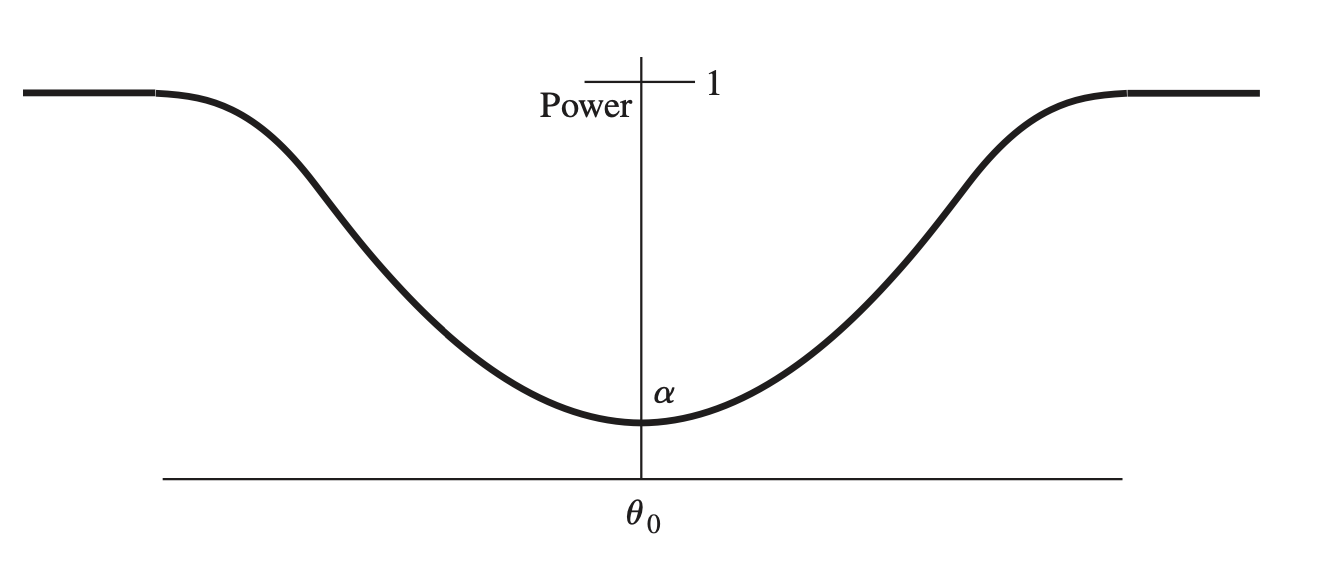
\includegraphics[width = 0.6\textwidth]{powercurve.png}
    \end{center}
\end{figure}


\subsubsection*{P-value}

\begin{definition}{P-Value}{}
    Consider an observed test-statistic $t$ from unknown distribution $T$. Then the $p$-value $p$ is what the prior probability would be of observing a test-statistic value at least as ``extreme'' as $t$ if null hypothesis $H_0$ were true.
\end{definition}

Note that under the null hypothesis, the p-value is uniformly distributed over $[0,1]$. For simplicity, consider a one-sided t-test. Then $p = \operatorname{Pr}(T \geq t) = 1-F(t)$ where $F$ is the cdf of the distribution of the test statistic under $H_0$. The \emph{Probability Integral Transform} tells us that the random variable $Z_t :=  F(t)$ is uniformly distributed over $[0,1]$ for any cumulative distribution function.


\subsubsection*{Confidence Intervals}

CI show a set of ``compatible'' parameter values. A $(1-\alpha)$-confidence interval contain all parameter values for which a test at significance level $\alpha$ would fail to reject.


We can often solve for CIs analytically: Find all values of $\mu$, so that the test does \emph{not} reject, i.e.:
$$
\left|\frac{\sqrt{n}\left(\bar{x}_n-\mu\right)}{\partial_X}\right| \leq q t\left(n-1 ; 1-\frac{\alpha}{2}\right) \rightarrow \text { solve for } \mu
$$

Thus, $(1-\alpha)$-confidence interval is:
$$
\left(\bar{X}_{\mathrm{n}}-\mathrm{qt}\left(\mathrm{n}-1 ; 1-\frac{\alpha}{2}\right)\cdot \frac{\hat{\sigma}_X}{\sqrt{n}} ; \bar{X}_{\mathrm{n}}+\mathrm{qt}\left(\mathrm{n}-1 ; 1-\frac{\alpha}{2}\right)\cdot \frac{\hat{\sigma}_X}{\sqrt{n}}\right)
$$

\begin{itemize}
    \item Rule of thumb for 95\%-CI: $\left(\bar{X}_{\mathrm{n}}-2\cdot \frac{\partial_X}{\sqrt{n}} ; \bar{X}_{\mathrm{n}}+2\cdot \frac{\partial_X}{\sqrt{n}}\right)$
    \item A $(1-\alpha)$-confidence interval covers the true value with probability $(1-\alpha)$.
\end{itemize}

\subsubsection*{Multiple Testing}

Suppose we consider performing 100 T-tests at a significance level $\alpha = 0.05$. Even if there is no effect, we expect to find about 5 significant results. One way of correcting for this is considering a conservative test level such that the probability of at least one type-1 error is $\leq \alpha$. This is called a \textbf{Familywise Error Rate}.

One simple and conservative approach is the \textbf{Bonferroni correction}: test at level $\alpha / m$ if $m$ tests are performed.


\subsubsection{Measuring association}

Pearon correlation is a standardized measure of the covariance and measures linear association:
\begin{equation*}
    \rho_{X, Y}=\operatorname{Cor}(X, Y)=\frac{\operatorname{Cov}(X, Y)}{\sigma_X \cdot \sigma_Y}=\frac{\sigma_{X Y}}{\sigma_X \cdot \sigma_Y}
\end{equation*}

For inference, we may use the \emph{Fisher z-transform} which is given by
\begin{equation}\label{eq.ztransfo}
    Z:=\tanh ^{-1}(\widehat{\rho})=\frac{1}{2} \log \left(\frac{1+\widehat{\rho}}{1-\widehat{\rho}}\right)
\end{equation}

\begin{proposition}{}{}
    If $\mathbf{X}, \mathbf{Y}$ follows a multivariate normal distribution, then $Z$ as defined in \eqref{eq.ztransfo} is approximately
    \begin{equation*}
        Z \sim \mathcal{N}\left(\tanh ^{-1}(\rho), \frac{1}{n-3}\right)
    \end{equation*}
\end{proposition}

A 95\%-CI for $\rho$ is thus given by
\begin{equation*}
    \tanh \left(z \pm 1.96 \cdot \sqrt{\frac{1}{n-3}}\right)
\end{equation*}

If we want to measure nonlinear associations as well, one possiblility is \textbf{Spearman correlation} which measures montone relationships. $r_S$ can be obtained by computing ranks and then applying Pearson correlation, or using
\begin{equation*}
    r_S=1-\frac{6 \sum_{i=1}^n D_i^2}{n\left(n^2-1\right)}, \quad D_i:=\operatorname{rank}\left(x_i\right)-\operatorname{rank}\left(y_i\right)
\end{equation*}


\subsubsection*{Simple Linear Regression}

Consider estimating a linear relation between pairs of variables $(x_i, Y_i)$: I.e., we want to find a line of the form $Y_i = \beta_0 + \beta_1 x_i$ that is as close as possible to $y_i$. We can fit our model by minimizing the sum of squared residuals, i.e.,
\begin{equation*}
    \widehat{\beta_0}, \widehat{\beta_1} = \arg \min \sum_{i=1}^n\left(y_i-\left(\beta_0+\beta_1 x_i\right)\right)^2
\end{equation*}

The solution is given by
\begin{equation*}
    \hat{\beta}_1=\hat{\rho}_{X Y} \cdot \frac{\widehat{\sigma}_Y}{\hat{\sigma}_X}, \quad \hat{\beta}_0=\bar{y}_n-\hat{\beta}_1 \bar{x}_n
\end{equation*}



\clearpage

\section{Estimating the Linear Regression Model}

Assume $X$ are fixed and $\operatorname{rank}(X) = p$ where $p$ is the number of predictors (including the intercept). Then
\begin{equation*}
    Y_i = \beta_1 + \beta_2 X_i^{(2)} + \ldots + + \beta_p X_i^{(p)} + \epsilon_i
\end{equation*}
We may write our regression equation in vector or matrix form as
\begin{equation*}
    \begin{aligned}
        &Y_i=X_i^\top \beta+\varepsilon_i, \\
        &Y=X \beta+\varepsilon
    \end{aligned}
\end{equation*}
with $\mathbb{E}\left(\varepsilon_i\right)=0, \operatorname{Var}\left(\varepsilon_i\right)<\infty$.

One way to estimate $\hat{\beta}$ from data is by minimizing the residual sum of squares:
\begin{equation*}
    \min \sum_{i=1}^{n} \left(Y_i - X_i^\top \beta\right)^2
\end{equation*}
This problem is equivalent to MLE with $\epsilon \sim \mathcal{N}(0, \sigma^2 \mathbf{1})$.

In matrix notation, we may write the objective function as
\begin{equation*}
    (Y-X\beta)^\top (Y-X\beta)
\end{equation*}
Taking gradient and setting equal to zero yields the normal equations:
\begin{equation*}
    X^T(Y-X \hat{\beta})=0 \rightarrow X^T X \hat{\beta}=X^T Y
\end{equation*}
The closed-form solution is then given by
\begin{equation}\label{eq.betahat}
    \hat{\beta}=\left(X^T X\right)^{-1} X^T Y
\end{equation}

To see equivalence between OLS and MLE under $\epsilon \sim \mathcal{N}$, note that the log likelihood of our data is given by
\begin{equation*}
    \log L=-n \cdot \log (\sigma \sqrt{2 \pi})-\frac{1}{2} \frac{\left(\sum_{i=1}^n\left(y_i-\beta_0-\beta_1 x_{1, i}-\cdots-\beta_{p-1} x_{p-1, i}\right)^2\right)}{\sigma^2}
\end{equation*}
clearly this quantitiy is maximized when the sum of squared residuals is minimized. One can also see from the quadratic function that we have a convex (or concave) optimization problem.



\subsection{Variable transformations}

Linear regression only requries linearity in parameters. We can for instance apply complex transformations to our $X$ columns and our target variable $Y$.

We often encounter the following variable transformations in our regression models:
\begin{enumerate}
    \item \textbf{Exponential type}:
    \begin{equation*}
        y=\exp \left(\beta_0+\beta_1 \cdot x\right) \cdot \tilde{\varepsilon} \rightarrow \tilde{y}=\beta_0+\beta_1 \cdot x+\varepsilon \text { with } \tilde{y}=\log (y)
    \end{equation*}
    \item \textbf{Power type}:
    \begin{equation*}
        y=\beta_0 \cdot x^{\beta_1} \cdot \tilde{\varepsilon} \rightarrow \tilde{y}=\widetilde{\beta_0}+\beta_1 \cdot \tilde{x}+\varepsilon
    \end{equation*}
    with $\tilde{y}=\log (y), \tilde{x}=\log (x), \widetilde{\beta_0}=\log \left(\beta_0\right)$
\end{enumerate}
In both case, we initially have a multiplicative error which we transform into an additive error.

Note, in general $g^{-1} \left(\mathbb{E}(g(Y))\right) \neq \mathbb{E}(Y)$. In particular, $\exp (E(\log (Y))) \neq E(Y)$. We therefore need to be careful when interpreting the results of our transformed equation back on the original scale.

However, if our distribution on the transformed scale is symmetric and since logarithms preserve ordering, $\mathbb{E}(\log(Y)) = \operatorname{median}(\log(Y)) = \log (\operatorname{median}(Y))$. Thus, $\exp (\mathbb{E}(\log (Y)))=\operatorname{median}(Y)$. The effect interpretation of our coefficient is then
\begin{equation*}
    \frac{\exp \left(E\left(\log (Y) \mid x_i+1\right)\right)}{\exp \left(E\left(\log (Y) \mid x_i\right)\right)}=\exp \left(\tilde{\beta_1}\right)=\frac{\operatorname{Median}\left(Y \mid x_i+1\right)}{\operatorname{Median}\left(Y \mid x_i\right)}
\end{equation*}
I.e., ``It is estimated that the median of $Y$ given $x_i+1$ is $\exp \left(\tilde{\mathbf{\beta}_1}\right)$ times as large as the median of $Y$ given $x_i$.''



\subsection{Linear Regression as Orthogonal Projection}

If we interpret our data in $X$ `column-wise', our columns are vectors spanning a ($p$-dimensional) subspace of $\mathbb{R}^n$.\footnote{Alternatively, we can interpret our data and regression `row-wise' in which our features and target are each a different basis of $\mathbb{R}^{p+1}$. We then want to fit a hyperplane that is as close as possible to all of our points.} I.e., the vector $Y$ of observations is a single point in the $n$-dimensional space $\mathbb{R}^n$. If we vary the value of the parameter $\mathbf{\beta}$, the product $X \mathbf{\beta}$ describes a $p$-dimensional hyperplane through the origin.

We can obtain our OLS estimates by trying to find the element $X \beta$ on the hyperplane which lies closest to the point $Y$. I.e.,
\begin{equation*}
    \text { Choose } \beta \text { to minimize } L_2 \text {-norm: }|Y-X \beta|_2{ }^2
\end{equation*}

\begin{figure}
    \caption{Graphical Intuition for Linear Regression as Projection}
    \label{fig:orth_linreg}
    \begin{center}
        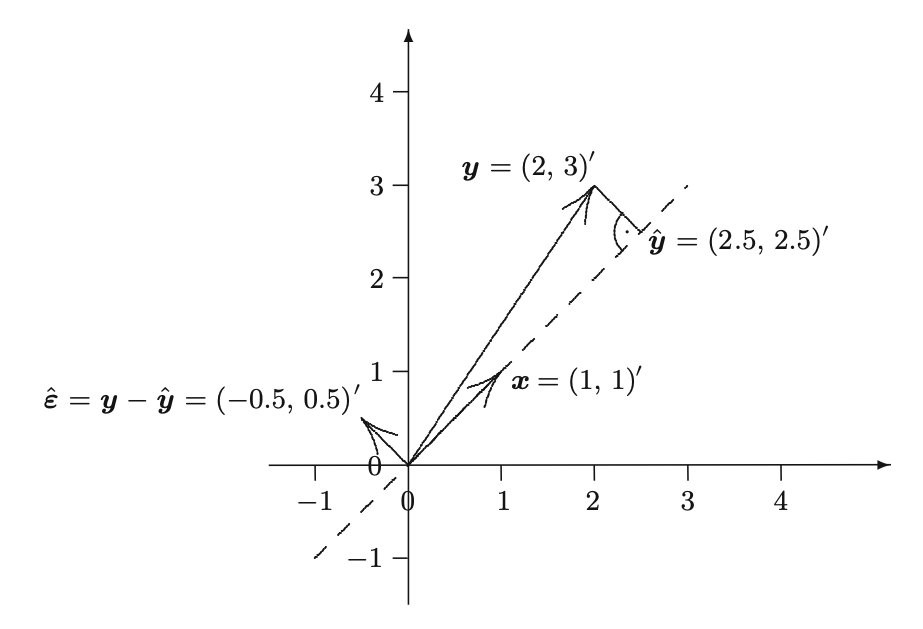
\includegraphics[width = 0.8\textwidth]{regression_orthogonal.png}
    \end{center}
\end{figure}

Since we obtain the orthogonal projection of $Y$ onto hyperplane spanned by columns of $X$, the residual vector $\hat{\varepsilon} = y - X \hat{\beta}$ must be orthogonal to any vector in the hyperplane, see Figure \ref{fig:orth_linreg} for an illustration. With this, we recover the normal equations $X^T(Y- X \hat{\beta}) = 0$. Solving for $\hat{\beta}$ yields
\begin{equation*}
    \hat{\beta}=\left(X^T X\right)^{-1} X^T Y
\end{equation*}

Our projection of $Y$ onto this subspace is therefore
\begin{equation*}
    \hat{Y}=X \hat{\beta}=\underbrace{X\left(X^T X\right)^{-1} X^T}_{:= H} Y= H Y
\end{equation*}
Note that $H$ has the exact form of the orthogonal projection matrix in \eqref{eq:orth_proj_matrix}.

If we want to obtain our residuals, we can do so by using the matrix $M = 1-H$, since
\begin{equation*}
    MY = (1-H) Y = Y-\hat{Y} = \hat{\varepsilon}
\end{equation*}
This is also a projection matrix. We also know (assuming $\epsilon \sim \mathcal{N}(0, \sigma^2 \mathbb{I})$)
\begin{equation}
    \hat{Y} \perp \hat{\varepsilon} \text{ since } H \cdot M = 0
\end{equation}
which follows from Lemma \ref{lma:indep_orthog_norm}. Also,
\begin{equation}\label{eq_xteps0}
    X^T \hat{\varepsilon} = 0.
\end{equation}
Intuitively, we can see \eqref{eq_xteps0} by noting that $\hat{\varepsilon}$ is orthogonal to the column space of $X$. Formally, we can show this as
$$
\begin{aligned}
    X^T \hat{\varepsilon} &= X^T(y- \hat{y}) \\
    &= X^T(1-H)y \\
    &= X^T (1 - X (X^TX)^{-1} X^T)y \\
    &= X^T y - (X^TX) (X^TX) ^{-1} X^T y \\
    &= 0
\end{aligned}
$$

This result leads to the following useful consequences:

\begin{itemize}
    \item $\hat{\beta} \perp \hat{\varepsilon}$
    \item $\hat{\varepsilon} = MY = M(X \beta + \varepsilon) = M \varepsilon$
    \item If our model includes an intercept, one column of $X$ is $E = (1,1, \ldots, 1)^T$. Thus
    \begin{equation*}
        E \cdot \hat{\varepsilon} = \sum \hat{\varepsilon}_i = 0
    \end{equation*}
    \item $\frac{1}{n} \sum_{i=1}^n \hat{y}_i=\bar{y} .$
    \item The regression hyperplane runs through the average of the data, i.e.,
    \begin{equation*}
        \bar{y}=\hat{\beta}_0+\hat{\beta}_1 \bar{x}_1+\cdots+\hat{\beta}_k \bar{x}_k .
    \end{equation*}
\end{itemize}

For the first of the above results, note
\begin{equation*}
    \hat{\beta}=\left(X^T X\right)^{-1} X^T Y=\left(X^T X\right)^{-1} X^T(\hat{Y}+\hat{\varepsilon})=\left(X^T X\right)^{-1} X^T \hat{Y}
\end{equation*}
so $\hat{\beta}$ is only a function of $X$ and $\hat{Y}$ and $\hat{Y} \perp \hat{\varepsilon}$.

Our projection interpretation allows us to perform the following Pythagoras decomposition:
\begin{equation*}
	R^2=1-\frac{R S S}{T S S}=\frac{E S S}{T S S}
\end{equation*}
\begin{itemize}
    \item Called \emph{coefficient of determination}
    \item Measure of goodness of fit
    \item Note that $|\hat{Y}-\bar{Y}|$ lies in the column space of $X$ and $|Y-\hat{Y}|$ lies in the orthogonal complement. Thus these two vectors are two sides to a right-angled triangle so
    \begin{equation*}
        TSS = ESS + RSS
    \end{equation*}
    where $TSS = |Y-\bar{Y}|^2$
    \item One can show that $R^2 = \left[cor(Y, \hat{Y})\right]^2$.
\end{itemize}



\subsection{Simple vs Multiple Regression and Partial Correlation}


Unless predictors are orthogonal, many simple regressions will yield different coefficient from multiple regression. Interpretation of multiple regression: Effect of $x_k$ on $Y$ when keeping $x_{-k}$ fixed.


Special case: Orthogonal design
\begin{itemize}
    \item Orthogonal predictors: $x_{., j}^{\top} x_{., k}=0$ for all $j \neq k$
    \item $X^T X=\operatorname{diag}\left(\sum_{i=1}^n x_{i, 1}^2, \ldots, \sum_{i=1}^n x_{i, p}^2\right)$
    Thus:
    $$\hat{\beta}_j=\left(\left(X^T X\right)^{-1} X^T Y\right)_j=\frac{\sum_{i=1}^n x_{i, j} y_i}{\sum_{i=1}^n x_{i, j}^2}=\frac{\widehat{\sigma}_{x_j, y}}{\hat{\sigma}_{x_j}^2}$$
    which is the  same result as simple regressions
\end{itemize}

We can therefore view multiple regression as measuring \emph{partial correlation}. An informal definiton of partial correlation is:

\begin{center}
    \textbf{Partial correlation} $\rho_{X Y \mid Z}$: strength and direction of the linear dependence between $X$ and $Y$ after accounting for the linear dependence of $X$ and $Y$ on $Z$
\end{center}

One can estimate partial correlation in the following ways:
\begin{enumerate}
    \item A recursive formula
    \item Let $r_x$ be residuals when regressing $x$ on $z$, $r_y$ residuals when regressing $y$ on $z$, then $\rho_{X Y \mid Z}=\operatorname{cor}\left(r_x, r_y\right)$
    \item Via precision matrix, $\rho_{Y X^j}{ }_{\mid X^{-j}}=-\frac{K_{p+1, j}}{\sqrt{K_{p+1, p+1} K_{j, j}}}$ where $K=\Sigma^{-1}$ and $\Sigma=\operatorname{Cov}\left(\left(X_{*, 1}, \ldots, X_{*, p}, Y\right)^T\right)$
\end{enumerate}

In multiple linear regression, we can write our estimated coefficients using partial correlation as
\begin{equation}\label{eq.betapartial}
    \beta_j=-\frac{K_{p+1, j}}{K_{p+1, p+1}}; \quad \rho_{Y X^j \mid X^{-j}}=\beta_j \frac{\sqrt{K_{p+1, p+1}}}{\sqrt{K_{j, j}}}
\end{equation}





\subsection{Computational considerations for estimating linear regression}


Instead of directly using the closed-form solution in \eqref{eq.betahat}, we can estimate the OLS coefficients in different ways. From \eqref{eq.betapartial} we can see that we can estimate them using partial correlations. The numerically prefered way is using a $QR$ decomposition of $X$. I.e., let $X = QR$ where $Q$ is $n \times p$ with orthonormal columns and $R$ is $p \times p$ upper triangle. From the normal equations, we have
\begin{equation*}
    \begin{aligned}
        & X^T X \hat{\beta}=X^T y \\
        & (Q R)^T(Q R) \hat{\beta}=(Q R)^T y \\
        & R^T Q^T Q R \hat{\beta}=R^T Q^T y \\
        & R^T R \hat{\beta}=R^T Q^T y \\
        & R \hat{\beta}=Q^T y \\
        \implies &\hat{\beta}=R^{-1} Q^T y
    \end{aligned}
\end{equation*}




\subsection{Categorical Variables and ANOVA}

We can include categorical variables as predictors by using dummy encoding (i.e., factors).
\begin{itemize}
    \item E.g., we can allow for a different intercept between two groups, where $x_2$ is a binary variable:
    \begin{equation*}
        Y_i = \beta_0  + \beta_1 x_1 + \beta_2 \mathbf{1} (x_2 = 1)+ \epsilon_i
    \end{equation*}
    \item One reference level and $k-1$ binary dummies if we have $k$ categories.

    \item Contrasts to derive the intercept in differnt groups. Let $\ell = \begin{pmatrix}
        1 & 0& 1
    \end{pmatrix}^\top$. Then $\ell^\top \beta$ is the intercept for the group with $x_2 = 1$.
    \item Interactions to allow for different slopes between groups. E.g.,
    \begin{equation*}
        Y_i = \beta_0  + \beta_1 x_1 + \beta_2 \mathbf{1} (x_2 = 1)+ \beta_3 x_1 \cdot\mathbf{1} (x_2 = 1) + \epsilon_i
    \end{equation*}
\end{itemize}

Analysis of Variance (ANOVA) is a special case of linear regression which is closely related to categorical variables. We illustrate the idea behind ANOVA using a simple example.

Let $g = 4$ be the number of groups (or `treatments') and $p$ denote the number of observations per group which we assume to be the same in each group. Our null hypothesis is
\begin{equation*}
    H_0: \; \mu_1 = \mu_2 = \mu_3 = \mu_4
\end{equation*}
To test this, we calculate:

\begin{itemize}
    \item \textbf{Variation between groups}:
    \begin{equation*}
        S S_B=p \cdot \sum_{i=1}^g\left(\bar{Y}_{i .}-\bar{Y}_{. .}\right)^2
    \end{equation*}
    where $\bar{Y}_{..}$ is the overall mean of all of observations.

    \item \textbf{Variation within groups}:
    \begin{equation*}
        S S_W=\sum_{i=1}^g \sum_{j=1}^p\left(Y_{i j}-\bar{Y}_{i .}\right)^2
    \end{equation*}
\end{itemize}
Our test statistic is then approximately $\dfrac{SS_B}{SS_w}$ which follows an F-distribution under suitable assumptions. We reject our null if the variation between group averages is much larger than within group variation. The setup is illustrated in Figure \ref{fig:anova}.

\begin{figure}
    \caption{Example ANOVA setup}
    \label{fig:anova}
    \begin{center}
        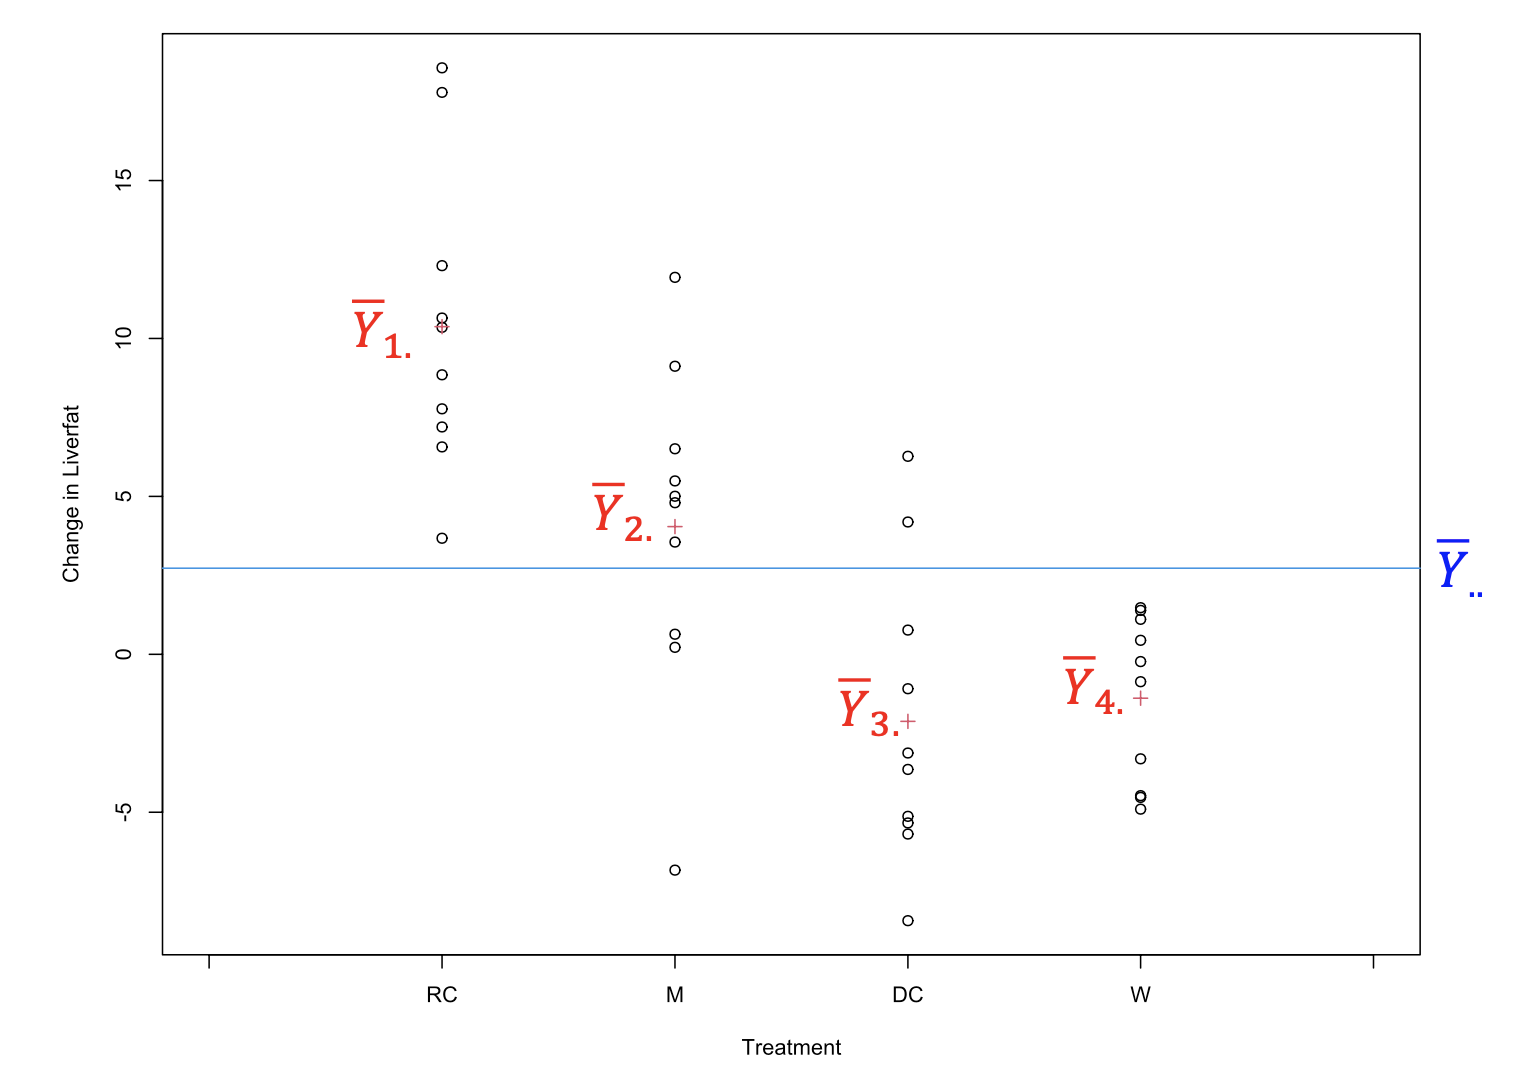
\includegraphics[width = 0.8\textwidth]{anova.png}
    \end{center}
\end{figure}


\clearpage

\section{Properties and Efficiency of OLS Estimates}

Note that our coefficients depend on $Y$ and, as $Y$ is random, are random variables themselves. We must therefore think about precision and distribution of estimated parameters. We assume the \emph{Gauss-Markov Conditions}:
\begin{equation*}
    \begin{aligned}
        & Y=X \beta+\varepsilon \\
        & E(\varepsilon)=0, \operatorname{Cov}(\varepsilon)=\sigma^2 I
    \end{aligned}
\end{equation*}

We obtain the following moments:

\begin{itemize}
    \item $\hat{\beta}$:
    \begin{itemize}
        \item $\mathbb{E} \left[ \hat{\beta}\right] = \beta$
        \item $\operatorname{Cov} \left( \hat{\beta}\right) = \sigma^2 (X^T X)^{-1}$
    \end{itemize}
    \item $\hat{Y}$:
    \begin{itemize}
        \item $\mathbb{E} \left[ \hat{Y}\right] = \mathbb{E} \left[ Y\right] = X\beta$
        \item $\operatorname{Cov} \left( \hat{Y}\right) = \sigma^2H$
    \end{itemize}
    \item $\hat{\varepsilon}$:
    \begin{itemize}
        \item $\mathbb{E} \left[ \hat{\varepsilon}\right]=0$
        \item $\operatorname{Cov} \left( \hat{\varepsilon}\right) = \sigma^2 M$ which implies $\operatorname{Var}(\hat{\epsilon}_i) = \sigma^2 (1 - H_{ii})$
        \item $\operatorname{Cov} \left( \hat{\varepsilon}, \hat{Y}\right) = 0$
    \end{itemize}
\end{itemize}


For the variance of a single element of our coefficient vector, one can obtain the following formula
\begin{equation*}
    \operatorname{Var}\left(\hat{\beta}_j\right)=\frac{\sigma^2}{\left(1-R_j^2\right) \sum_{i=1}^n\left(x_{i j}-\bar{x}_j\right)^2},
\end{equation*}
where $R^2_j$ is the coefficient of determination from regressing $x_j$ as the response on all other variables in $X$. We note:

\begin{itemize}
    \item The smaller the model variance $\sigma^2$, the smaller the variance of $\hat{\beta}_j$ and thus the more accurate the estimation.
    \item The smaller the linear dependence between $x_j$ and the other explanatory variables (measured through $R_j^2$ ), the smaller is the variance of $\hat{\beta}_j$. The variance, $\operatorname{Var}\left(\hat{\beta}_j\right)$, is minimized for $R_j^2=0$, i.e., when the covariates are uncorrelated.
    \item The larger the variability of covariate $x_j$ around its average, the smaller is the variance of $\hat{\beta}_j$.
\end{itemize}

Further, we can show that $1/(n-p) \sum_{i=1}^{n} \hat{\epsilon}_i^2$ is an unbiased estimate of $\sigma^2$. To this end, note that
\begin{equation*}
    \begin{aligned}
        \mathbb{E} \left[\hat{\sigma}^2\right]&=\frac{1}{n-p} \sum_{i=1}^{n} \mathbb{E} \left[ \hat{\epsilon}_i^2\right] =\frac{1}{n-p} \sum_{i=1}^{n} \operatorname{Var} \left[ \hat{\epsilon}_i^2\right] \\
        &=\frac{1}{n-p} \sum_{i=1}^{n} \sigma^2 (1-H_{ii})=\frac{1}{n-p} \sigma^2 \left(n- \operatorname{tr}({H})\right) \\
        &=\frac{1}{n-p}  \sigma^2 \left( n - \operatorname{tr}(X (X^TX)^{-1} X)\right) \\
        &=\frac{1}{n-p}  \sigma^2 \left( n - \operatorname{tr}(\mathbf{1}_{p\times p})\right)=\sigma^2
    \end{aligned}
\end{equation*}

Note here also the following insight into the relation between degrees of freedom and projection matrices:
\begin{itemize}
    \item We have $n$ observations and estimate $p$ parameters to obtain residuals. Thus residual df are $n-p$
    \item The trace of a projection matrix measures the rank of the subspace onto which it projects a vector. I.e., how many independent dimensions there are in a subspace. We have $\operatorname{tr}(M) = tr(\mathbf{1}-H) = n-p.$
\end{itemize}

\subsection{Gauss-Markov Theorem}

Given data $Y$, a parameter estimate in general is some function $\hat{\beta} = f(Y)$. We want to understand goodness properties of OLS and how (or, whether) there are ways to improve upon OLS.

Note that OLS has the following properties

\begin{enumerate}
    \item $\hat{\beta} = (X^T X)^{-1} X^T y = Ay$ is \emph{linear}
    \item  $\mathbb{E}(\hat{\beta}) = \beta$, i.e., \emph{unbiased}
\end{enumerate}

We will show that, depending on more or less restrictive assumptions, OLS can be
\begin{itemize}
    \item Optimal among all \emph{unbiased estimators}, and
    \item Optimal among all \emph{linear and unbiased} estimators.
\end{itemize}
In both cases we may obtain an estimator with lower MSE by allowing for small bias if we can achieve a large reduction of variance simultaneously, see equation \eqref{eq:mse_bias_var}.

These results and the underlying assumptions are summarised in the following two theorems.

\begin{theorem}{Gauss-Markov -- Version 1}{gaus_markov_1}
    Let $Y=X \beta+\varepsilon, E(\varepsilon)=0, \operatorname{Cov}(\varepsilon)=\sigma^2 I, r n k(X)=p$. Furthermore, let $\ell \in \mathbb{R}^p$, and $\hat{\beta}$ the OLS estimator.

    Then, for all $c \in \mathbb{R}^n$ such that $E\left(c^T y\right)=\ell^T \beta$, we have: $$\operatorname{Var}\left(\ell^T \hat{\beta}\right) \leq \operatorname{Var}\left(c^T y\right).$$
\end{theorem}

Thus, the OLS estimator $\ell^T \hat{\beta}$ has minimal variance among all linear unbiased estimators of $\ell^T \beta$.

\begin{proof}
    Let $y \in \mathbb{R}^n, X \in \mathbb{R}^{n \times p}, \beta \in \mathbb{R}^p$. The OLS estimator is given by
    $$
    \begin{aligned}
    &\hat{\beta} = \left( X^T X \right)^{-1} X^T y \\
    &\implies \ell^T \hat{\beta} = \ell^T \left( X^TX \right)^{-1} X^T y
    \end{aligned}
    $$

    We know that $\mathbb{E} \left[ \ell^T \hat{\beta}\right] = \ell^T \beta$. Now let $c^T y$ be any other linear unbiased estimator of $\ell^T \beta$. Since this estimator is unbiased,
    $$
    \ell^\top \beta = \mathbb{E} \left[ c^T y\right]= c^T X \beta
    $$
    so that we must have $\ell^T = c^T X$.

    We now consider variances.
    $$
    \begin{aligned}
    \operatorname{Var} \left( c^T y\right)&= \sigma^2 c^T c \\
    \operatorname{Var} \left( \ell^T \beta\right) &= \sigma^2 \ell^T \left( X^T X \right)^{-1} \ell \\
    &= \sigma^2 c^T X \left( X^T X \right)^{-1} X^T c
    \end{aligned}
    $$

    Subtracting both variances, we obtain
    $$
    \begin{aligned}
    &\operatorname{Var} \left( c^T y\right) - \operatorname{Var} \left( \ell^T \beta\right) \\
    &=
    \sigma^2 c^T \left( 1 - X^T \left( X^T X \right)^{-1}  X^T  \right) c\\
    &= \sigma^2 c^T M c \geq 0
    \end{aligned}
    $$
    since $M$ is positive semi-definite.\footnote{Since $M$ is a orthogonal projection, $M^T = M = M^2$. Let $z$ be any vector of appropriate dimensions, then
    \begin{equation*}
        z^T M z = z^T M^T M z = (M z)^T M z = \left|M z\right|^2 \geq 0
    \end{equation*}
       }
\end{proof}

If we are further willing to assume normality of the error term, we arrive at a stronger result.

\begin{theorem}{Gauss-Markov -- Version 2}{gaus_markov_2}
    Let furthermore $\varepsilon$ be normally distributed. Then $\ell^T \hat{\beta}$ has minimal variance among all unbiased estimators of $\ell^T \beta$.
\end{theorem}

To proof the above theorem, we will use the Cramer-Rao bound result:

Let $\left(f_{\mathbf{\eta}}(\mathbf{Y})\right)$ be a parametric family of strictly positive densities in $\mathbb{R}^n$. Let $\mathbf{\eta}$ be a variable parameter with values in an open subset of $\mathbb{R}^k$, and let $f_{\mathbf{\eta}}(\mathbf{Y})$ be differentiable wrt $\mathbf{\eta}$. Our parameter of interest is $g(\mathbf{\eta})$, where $g$ is an arbitrary real-valued function of $\mathbf{\eta}$. Then we obtain the following result:

\begin{theorem}{Cramér-Rao for unbiased estimators}{}
    If $T(\mathbf{Y})$ is an arbitrary unbiased estimate of $g(\mathbf{\eta})$, i.e.
    $$
    \mathbb{E}_{\mathbf{\eta}}[T(\mathbf{Y})]=g(\mathbf{\eta}) \quad \forall \mathbf{\eta},
    $$
    then $g$ is differentiable and

    \begin{equation}\label{eq:cramerrao_proof_to}
        \operatorname{Var}_{\mathbf{\eta}}(T(\mathbf{Y})) \geq \frac{\partial g^T}{\partial \mathbf{\eta}} I(\mathbf{\eta})^{-1} \frac{\partial g}{\partial \mathbf{\eta}}
    \end{equation}
    where $I(\mathbf{\eta})$ denotes the Fisher information matrix:
    \begin{equation*}
        I(\mathbf{\eta})=\mathbb{E}_{\mathbf{\eta}}\left[\frac{\partial \log f_{\mathbf{\eta}}(\mathbf{Y})}{\partial \mathbf{\eta}} \frac{\partial \log f_{\mathbf{\eta}}(\mathbf{Y})^T}{\partial \mathbf{\eta}}\right] .
    \end{equation*}
\end{theorem}

\begin{proof}
    We know that
    \begin{equation}\label{eq:var_ols}
        \operatorname{Var} \left( \ell^T \beta\right) = \ell^T \sigma^2 (X^TX)^{-1}  \ell
    \end{equation}

    We now derive the Cramer-Rao lower bound. We have $\eta = (\sigma^2, \beta^T)^T$ and $g(\eta)=\ell^T \beta$. Then the Fisher information matrix is given by
    $$
    I(\eta) = \mathbb{E}_\eta \left[ \nabla_\eta \log L \cdot \nabla_\eta \log L^T \right]
    $$
    where we use $\log L$ to denote the log likelihood function.

    Our log likelihood function is
    \begin{equation*}
        \log L=\sum_{i=1}^{N} -\frac{1}{2} \log \left(2 \pi \sigma^2\right)-\frac{\left(y_i-x_i^T \beta\right)^2}{2 \sigma^2}
    \end{equation*}


    Taking derivatives,
    \begin{equation}\label{eq.pardev}
        \nabla_\eta \log L=
        \begin{bmatrix}
            \sum_{i=1}^N\left(-\frac{1}{2 \sigma^2}+\frac{\left(y_i-x_i^T \beta\right)^2}{2 \sigma^4}\right) \\
            \sum_{i=1}^N\left(\frac{\left(y_i-x_i^T \beta\right) x_i}{\sigma^2}\right)
        \end{bmatrix}
    \end{equation}
    Since observations are independent, the Fisher information matrix is the sum of the individual Fisher information matrices for single observations. We compute,
    $$
    \begin{aligned}
        I_{11}^{(i)}&=\mathbb{E}\left[\left(-\frac{1}{2 \sigma^2}+\frac{\left(y_i-x_i^T \beta\right)^2}{2 \sigma^4}\right)^2\right]=\frac{1}{2 \sigma^4} \\
        I_{j k}^{(i)}&=\mathbb{E}\left[\frac{\left(y_i-x_i^T \beta\right)^2 x_j x_k}{\sigma^4}\right]=\frac{x_j x_k}{\sigma^2} \\
        I_{1 j}^{(i)}&=I_{j 1}^{(i)}=\mathbb{E}_\eta\left[\left(-\frac{1}{2 \sigma^2}+\frac{\left(y-x^T \beta\right)^2}{2 \sigma^4}\right) \cdot \frac{\left(y-x^T \beta\right) \cdot x_j}{\sigma^2}\right]=0
    \end{aligned}
    $$
    For the first result, we use $\mathbb{E}\left[\left(y_i-x_i^T \beta\right)^4\right]=3 \sigma^4$ for the normal distribution. In the last result, after extending and simplyfing, we again use this result and the unbiasedness of our estimate.

    Summing over all observations, we arrive at
    $$
    I(\eta) =
    \begin{bmatrix}
    \frac{n}{2 \sigma^4} & 0  \\
    0 & \frac{1}{\sigma^2} X^TX
    \end{bmatrix}
    $$
    Taking the inverse of this block matrix, we get
    $$
    I(\eta)^{-1} =
    \begin{bmatrix}
    \frac{2}{n} \sigma^4 & 0  \\
    0& \sigma^2 (X^TX)^{-1}
    \end{bmatrix}
    $$

    We compute the gradient vectors:
    \begin{equation*}
        \frac{\partial g}{\partial \eta}
        =
        \begin{bmatrix}
            \partial \ell^T \beta / \partial \sigma^2 \\
            \partial \ell^T \beta / \partial \beta_1 \\
            \vdots \\
            \partial \ell^T \beta / \partial \beta_p
        \end{bmatrix}
        =
        \begin{bmatrix}
            0 \\
            \ell_1 \\
            \vdots \\
            \ell_p
        \end{bmatrix}
        =
        \begin{bmatrix}
            0 \\
            \ell
        \end{bmatrix}
    \end{equation*}


    Finally, multiplying out, we obtain
    $$
    \frac{\partial g^T}{\partial \eta} I(\eta)^{-1}  \frac{\partial g}{\partial \eta} = \ell^T \sigma^2 \left( X^T X \right)^{-1} \ell
    $$
    so that our OLS estimator's variance in \eqref{eq:var_ols} achieves the Cramer-Rao lower bound in \eqref{eq:cramerrao_proof_to}.
\end{proof}

Note that there may be biased estimators which yield a lower mean squared error. In particular, the MSE can be decomposed as
\begin{equation}\label{eq:mse_bias_var}
    \left.\mathbb{E}\left((\hat{\theta}-\theta)^2\right)=(\mathbb{E}(\hat{\theta})-\theta)^2+\operatorname{Var}(\hat{\theta})\right)
\end{equation}

When may our OLS estimates perform badly?

\begin{itemize}
    \item If our normality assumption holds, one may obtain slightly biased estimators with far lower variance
    \item If normality assumption is violated, OLS and MLE no longer coincide so we no longer have asymptotic efficiency. Non-linear estimates may outperform OLS.
\end{itemize}


\subsection{Distribution of $\hat{\beta}$}

\subsubsection*{Normal errors}

Under normal errors, MLE coincides with OLS, so we should expect asymptotic nromallity of our estimated coefficients. We can, however, show that this already holds in finite samples.


\begin{proposition}{}{var_disr_n}
    Assume that $Y = X \beta + \varepsilon$ with $\varepsilon \sim \mathcal{N}(0, \sigma^2 \mathbb{I})$. Then

    \begin{enumerate}
        \item $\widehat{\mathbf{\beta}} \sim \mathcal{N}_p\left(\mathbf{\beta}, \sigma^2\left(X^T X\right)^{-1}\right) \quad$
        \item $\widehat{\mathrm{Y}} \sim \mathcal{N}_n\left(X \mathbf{\beta}, \sigma^2 H\right), \quad \widehat{\varepsilon} \sim \mathcal{N}_n\left(\mathbf{0}, \sigma^2 M\right)$
        \item $\widehat{\mathrm{Y}}$ and $\widehat{\varepsilon}$ are independent
        \item $\frac{\sum_{i=1}^n \hat{\varepsilon}_i^2}{\sigma^2} \sim \chi_{n-p}^2$
        \item $\widehat{\sigma}^2$ is independent of $\widehat{\mathbf{\beta}}=\left(X^T X\right)^{-1} X^T Y$
    \end{enumerate}
\end{proposition}

Note that result 2) implies that even though $\varepsilon$ are i.i.d., the covariance structure of $\hat{\varepsilon}$ can be highly dependent, including heteroskedasticity.

\begin{proof}

    \emph{1.)}
    Since $Y \sim N(X \beta, \sigma^2 \mathbb{I})$ and $\hat{\beta}=(X^T X)^{-1} X^T y$, this implies that $\hat{\beta} \sim N(.,.)$. Note that

$$
\mathbb{E} \left[ \hat{\beta}\right] = (X^T X)^{-1} X^T \mathbb{E} \left[ y\right] = (X^TX)^{-1} X^T (X \beta + \mathbb{E} \left[ \varepsilon\right]) = \beta
$$

and

$$
\operatorname{Var} \left( \hat{\beta}\right)= \left[ (X^TX)^{-1} X^T \right] \operatorname{Var} \left( y\right) \left[ (X^TX)^{-1} X^T \right]^T = \sigma^2 (X^T X)^{-1}
$$

\emph{2.)}

$\hat{Y} = HY$ where $H = X(X^TX) ^{-1}X^T$ with rank$(H) = p$. Thus $\hat{Y} \sim N(.,.)$.  We have

$$
\mathbb{E} \left[ \hat{Y}\right] = H \mathbb{E} \left[ Y\right] = HX\beta = X \beta = \mathbb{E} \left[ Y\right]
$$

This follows since $H$ is a projection onto the column space of $X$ and $X \beta$ evidently already lies in the col. space of $X$. Also,
$$
\operatorname{Var} \left( \hat{Y}\right) = H \operatorname{Var} \left( Y\right) H^T = \sigma^2 H H^T = \sigma^2 H
$$

$\hat{\varepsilon} = MY$ where $M = \mathbb{I}-H$.
\begin{align*}
    \mathbb{E} \left[ \hat{\varepsilon}\right] &= M \mathbb{E} \left[ y\right] = MX\beta = (\mathbb{I}-H) X \beta = 0 \\
    \operatorname{Var} \left( \hat{\varepsilon}\right) &= \operatorname{Var} \left( MY\right) = \sigma^2 M
\end{align*}

\emph{3.)}

$\hat{Y} = HY, \hat{\varepsilon} = MY$. Note that

$$
HM = 0
$$

Thus, by Lemma \ref{lma:indep_orthog_norm}, we have $\hat{Y} \perp \hat{\varepsilon}$

\emph{4.)}

Let $e_i = \hat{\varepsilon}_i / \sigma$. Then
$$
\frac{\sum \hat{\varepsilon}_i}{\sigma^2} = e^T e = e^T M e
$$
We can multiply by the matrix $M$ since $e$ lies in the orthogonal complement of the column space of $X$ and is therefore unaffected by multiplying with the orthogonal projection matrix $M$.

We know that $e_i \sim N, \mathbb{E} \left[ e\right] =0, \operatorname{Var} \left( e\right) = \frac{1}{\sigma^2} \operatorname{Var} (\hat{\epsilon}_i) = M$. Therefore, $e \sim \mathcal{N}(0, M)$. We also know that $M$ is idempotent and
$$
\operatorname{ rank } (M) = \operatorname{ rank } (\mathbb{I}-H) = n-p
$$
Then, using Lemma \ref{lma:chisquare_idem}, $e^T M e \sim \chi^2_{n-p}$.


\emph{5.)}

Since $X^T\hat{e} = 0$.
$$
\hat{\beta} = (X^T X)^{-1} X^T (\hat{Y} + \hat{\varepsilon}) = (X^TX)^{-1} X^T \hat{Y}.
$$
Thus, $\hat{\sigma}$ is a function of $\hat{\varepsilon}$ and $\hat{\beta}$ is a function of $\hat{Y}$. Since $\hat{Y} \perp \hat{\varepsilon}$, we also have $\hat{\beta} \perp \hat{\sigma}$.



\end{proof}




\subsubsection*{Gauss-Markov Assumptions}

We now turn to the case where the errors are iid but not normally distributed. In this case, OLS no longer coincides with MLE so we must consider the use of some central limit theorem to derive asymptotic normality. In particular, we will use the Lindernberg-Feller CLT:

\begin{theorem}{Lindenberg-Feller Central Limit Theorem}{lindfellclt}
    Suppose $\{ x_{ni} \}$ is a triangular array of $p \times 1$ random vectors such that $z_n = \frac{1}{n} \sum_{ i =1 }^{ n } x_{ni}$ and

    $$
    V_n = \frac{1}{n} \sum_{ i=1 }^{ n }  \operatorname{Var} \left( X_{ni}\right) \to V, \text{ where }V \text{ is psd.}
    $$
    If for every $\varepsilon > 0$ we have

    $$
    \frac{1}{n} \sum_{ i = 1 }^{ n } \mathbb{E} \bigg\{ ||x_{ni}||^2 \mathbf{1} \left( ||x_{ni}||  \geq \varepsilon \sqrt{ n } \right)  \bigg\} \to 0,
    $$
    then $\sqrt{ n } z_n \overset{d}{\to} \mathcal{N}(0,V)$. Or equivalently, $\sqrt{ n } V_n^{-1/2} z_n \overset{d}{\to} \mathcal{N}(0, \mathbb{I})$.
\end{theorem}

For the asymptotic approximation to hold, we need some weak conditions on the explanatory variables $\mathbf{x}_i$:

\begin{itemize}
    \item The smallest eigenvalue of $X^T X=\sum_{i=1}^n \mathbf{x}_i \mathbf{x}_i^T$, namely $\lambda_{\min , n}$, converges to $\infty$.
    \item $\max _j P_{j j}=\max _j \mathbf{x}_j^T\left(\sum_{i=1}^n \mathbf{x}_i \mathbf{x}_i^T\right)^{-1} \mathbf{x}_j$ converges to zero.
\end{itemize}

The first condition states that increasing $n$ always yields more information, while the second condition prohibits any $\mathrm{x}_j$ from dominating the others.

\begin{theorem}{Asymptotic normality of coefficients under Gauss-Markov}{asym_normal_betahat}
    If the errors $\varepsilon_i$ are i.i.d. with mean 0 and variance $\sigma^2$, and if $\left(\mathbf{x}_i\right)$ satisfies the conditions just given, then the LS estimators $\widehat{\mathbf{\beta}}$ are consistent (for $\mathbf{\beta}$), and the distribution of

    $$
    \left(X^T X\right)^{1 / 2}(\widehat{\mathbf{\beta}}-\mathbf{\beta})
    $$

    converges weakly to $\mathcal{N}_p\left(\mathbf{0}, \sigma^2 I\right)$.
\end{theorem}

We will proof a slightly easier version of the above statement, by assuming that $x_i^T x_i$ is bonded instead of the second assumption.

\begin{proof}

    \textbf{Consistency.}

    The $i$-th component $\widehat{\beta}_i$ is unbiased and has variance $\sigma^2\left(\left(X^T X\right)^{-1}\right)_{i i}$, which converges to zero by the first assumption. Then consistency follows from Chebyshev's inequality.

    \textbf{Asymptotic normality.}

    Suppose $y = X \beta + \omega$ where $\omega_i \sim F$ i.i.d with $\mathbb{E} \left[ \omega_i\right] = 0, \operatorname{Var} \left( \omega_i\right) = \sigma^2$. Suppose further that

    $$
    \frac{1}{n} X^T X \to \Sigma, \text{ where } \Sigma \text{ is psd}
    $$
    Let $x_i$ denote the fixed $p \times 1$ vector of covariates of observation $i$ and assume there exists $M \in \mathbb{R}$ such that $||x_i|| < M < \infty, \;\forall i$.

    \emph{Step 1: Rearrange OLS estimate}

    $$
    \begin{aligned}
    \hat{\beta} &= (X^T X)^{-1} X^T y = (X^T X)^{-1} X^T (X \beta + \omega) \\
    &= \beta + (X^T X)^{-1} X^T \omega
    \end{aligned}
    $$
    We can write
    $$
    X^T \omega = \sum_{ i = 1 }^{ n } x_i \omega_i
    $$
    That is, our estimate $\hat{\beta}$ is the true value plus some function of the noise term. While $\omega_i$ are iid, premultiplying with $x_i$ yields independently but not identically distributed RVs. We wish to show that this noise term is asymptotically normal.


    \emph{Step 2: Check Lindenberg-Feller Condition}

    We now consider the Lindenberg-Feller CLT.

    A triangular array is given by random variables in the form
    $$
    \begin{aligned}
    & x_{11} \curvearrowleft x_i \omega_i \\
    & x_{21}  \quad x_{22} \\
    & x_{31} \quad x_{32}  \quad x_{33} \\
    & \vdots \quad \quad \quad \ldots
    \end{aligned}
    $$
    where the RVs in each row are independent, have expected value zero, and have finite variances.

    We consider each element to be an element of $x_i \omega_i$. We can see that the conditions hold as $x_i \omega_i \perp x_j \omega_j$ since $\omega_i$ iid. and $x_i, x_j$ are assumed to be fixed, $\mathbb{E}(x_i \omega_i) = x_i \mathbb{E}(\omega_i) = 0$ and $\operatorname{Var}(x_i \omega_i) = \sigma^2 x_i  x_i^T < \infty$ by assumption.

    Thus, $x_i \omega_i$ is a triangular array with
    \begin{itemize}
        \item row-wise means: $z_n = \frac{1}{n} \sum x_i \omega_i = \frac{1}{n} X^T \omega$.
        \item row-wise average variance:
        \begin{equation}\label{eq.rowwisevar}
            V_n = \frac{1}{n} \sum_i \operatorname{Var} \left( x_i \omega_i \right) = \frac{1}{n} \sum \sigma^2 x_i x_i^T = \frac{\sigma^2}{n} X^T X \to \sigma^2 \Sigma
        \end{equation}
        where convergence follows by assumption.
    \end{itemize}

    We now turn to verify the LF-condition. Let $\varepsilon > 0$, recall that we assume existence of $M$ such that $||x_i|| < M, \;\forall i$.

    $$
    \begin{aligned}
    & \frac{1}{n} \sum_i E\left\{\left\|x_i \omega_i\right\|^2 \mathbf{1}\left(\left\|x_i \omega_i\right\| \geqslant \varepsilon \sqrt{n}\right)\right\} \\
    & =\frac{1}{n} \sum_i E\left\{\omega_i^2\left\|x_i\right\|^2 \mathbf{1}\left(\left|\omega_i\right|\left\|x_i\right\| \geqslant \varepsilon \sqrt{n}\right)\right\} \\
    & <\frac{1}{n} \sum_i E\left\{\omega_i^2 M^2 \mathbf{1}\left(\left|\omega_i\right| M \geqslant \varepsilon \sqrt{n}\right\}\right.  \\
    & =E\left\{\omega^2 M^2 \mathbf{1}(|\omega| M \geqslant \varepsilon \sqrt{n})\right\} \\
    & =: E\left\{T_n\right\}
    \end{aligned}
    $$
    Note that $T_n \overset{p}{\to} 0$ as $\varepsilon \sqrt{ n } M^{-1} \to \infty$ as $\omega$ are iid with finite variance.\footnote{If $\omega_i$ are iid with finite second moment, we have from Chebyshev's inequlity that
    \begin{equation*}
        \mathbb{E} \left[\omega_i^2 1_{\left[\left|\omega_i\right|>d\right]}\right]=\mathbb{E} \left[\omega_1^2 1_{\left[\left|\omega_1\right|>d\right]}\right] \xrightarrow{d \rightarrow \infty} 0 .
    \end{equation*}
     }

    Define $Z = M^2 \omega^2, \mathbb{E} \left[ Z\right] = M^2 \sigma^2 < \infty$. Note that $\;\forall n \in  \mathbb{N}: T_n \leq Z$. Since $T_n$ converges pointwise to the zero function and we have an integrable function which dominates $T_n$ we can apply the \emph{Dominated convergence theorem} to deduce convergence of $\mathbb{E}(T_n)$:
    $$
    T_n \overset{p}{\to} 0 \implies T_n \overset{d}{\to} 0 \implies \mathbb{E} \left[ T_n\right] \to 0
    $$
    \emph{3: Putting it all together}

    Recall:
    $$
    \begin{aligned}
    & \hat{\beta}=\beta+ (X^TX)^{-1}  X^T \omega \\
    &  z_n=\frac{1}{n} \sum x_i \omega_i=\frac{1}{n} X^T \omega \\
    & V_n=\frac{1}{n} \sum \operatorname{Var}\left(x_i \omega_i\right) \rightarrow \sigma^2 \Sigma
    \end{aligned}
    $$
    Then the LF-CLT says
    $$
    \sqrt{ n } z_n \overset{d}{\to} \mathcal{N}(0,V)
    $$
    Hence,
    $$
    \frac{1}{\sqrt{ n }} X^T \omega \overset{d}{\to} \mathcal{N}(0,\sigma^2 \Sigma)
    $$
    We know that $(X^T X) (\hat{\beta}- \beta) = X^T \omega$, thus (dividing by the square root of the variance from \eqref{eq.rowwisevar}), we normalise and obtain
    $$
    \frac{1}{\sigma} (X^TX)^{-1/2} (X^T X) (\hat{\beta} - \beta) = \frac{1}{\sigma} (X^TX) ^{1/2}(\hat{\beta}- \beta) \overset{d}{\to} \mathcal{N}(0,\mathbb{I})
    $$
\end{proof}




\subsection{Testing}

We next prove the distribution of various potential test statistics. Note that we always assume $\varepsilon \sim \mathcal{N}_n(0, \sigma^2 \mathbb{I}_{n \times n})$. In particular, p-values in summary outputs in R rely on this normality assumption. If instead only Gauss-Markov assumptions hold, p values and confidence intervals are only valid asymptotically.

\subsubsection*{Confidence interval for $\beta$}

\begin{proposition}{}{}
    Assume $\varepsilon \sim \mathcal{N}_n(0, \sigma^2 \mathbb{I}_{n \times n})$ then $\hat{\beta} \sim N_p (\beta, \sigma^2 (X^TX)^{-1})$. Further, let $\hat{\sigma}^2 = \frac{\sum \hat{\varepsilon}_i^2}{n-p}$. We have $\frac{\sum \hat{\varepsilon}_i^2}{\sigma^2}  \sim \chi^2_{n-p}$ and $\hat{\sigma} \perp \hat{\beta}$. Then:
    $$
    \frac{\hat{\beta}_i - \beta_i}{\hat{\sigma} \sqrt{ \left( \left( X^T X \right)^{-1}   \right)_{ii}  }} \sim t_{n-p}
    $$
\end{proposition}

\begin{proof}
    Recall, by definition of the t-distribution that if $Z \sim \mathcal{N}(0,1), V \sim \chi^2_n, Z \perp V$, then
    $$
    T = \frac{Z}{\sqrt{ V / n }} \sim t_n
    $$

    Since $\hat{\beta}_i \sim \mathcal{N} (\beta_i, \sigma^2 \left( (X^TX)^{-1} \right)_{ii})$, we have
    $$
    \begin{aligned}
    &Z = \frac{\hat{\beta}_i - \beta_i}{\sigma \sqrt{ \left( (X^TX)^{-1} \right)_{ii} }} \sim \mathcal{N}(0,1) \\
    &V = \frac{\sum \hat{\varepsilon}_i}{\sigma^2} \sim \chi^2_{n-p} \text{ and } V \perp Z
    \end{aligned}
    $$

    Thus
    $$
    T = \frac{\frac{\hat{\beta}_i - \beta_i}{\sigma \sqrt{ \left( (X^TX)^{-1} \right)_{ii} }}}{\sqrt{\frac{\sum {\hat{\varepsilon}_i}^{2}}{\sigma^2(n-p)}} } = \frac{\hat{\beta}_i - \beta_i}{\hat{\sigma} \sqrt{ \left( \left( X^T X \right)^{-1}   \right)_{ii}  }} \sim t_{n-p}.
    $$
    Here we used $\sum \hat{\varepsilon}_i^2 / (n-p) = \hat{\sigma}^2$.
\end{proof}

Using our typical `Wald-type-CI', we can achieve a $\alpha$ level CI by rewriting
\begin{equation*}
    \hat{\beta}_i - q_{t_{\alpha/2, n-p}} \hat{\sigma}_{\hat{\beta}_i} \leq \beta_i \leq \hat{\beta}_i + q_{t_{\alpha /2, n-p}} \hat{\sigma}_{\hat{\beta}_i}
\end{equation*}
where $\hat{\sigma}_{\hat{\beta}_i} = \hat{\sigma} \sqrt{ \left( \left( X^T X \right)^{-1}   \right)_{ii} }$.


\subsubsection*{Confidence Interval for $\mathbb{E}(Y)$}

The confidence interval for the expected value of $Y$ (i.e., confidence interval for the level of the regression line at a point), is entirely similar to above. Noting that
\begin{equation*}
    \hat{Y}_i \sim \mathcal{N}(\mu_i, \sigma^2 H_{ii})
\end{equation*}
where $H$ is the matrix used in $\hat{y} = Hy$, we obtain the test statistic
\begin{equation*}
    T = \frac{\hat{y}_i - \mu_i}{\hat{\sigma} \sqrt{H_{ii}}} \sim t_{n-p}.
\end{equation*}
The proof of the distribution follows our approach above.

\subsubsection*{Prediction interval}

If we want to have a confidence interval for the predicted interval of accuracy single observation, i.e., a \textbf{prediction interval}, we need to consider not only the source of uncertainty from a wrong estimate of $\beta$ but also the underlying noise in the data. Thus, prediction intervals are larger than the corresponding CI for $\mathbb{E} (\hat{Y})$.

$y_0 \perp \hat{y}_0$, since we consider a new observation $y_0 = x_0^T \beta + \varepsilon_0$ which was not used in the estimation of $\hat{\beta}$.

Consider $D = y_0 - \hat{y}_0 \sim \mathcal{N}(\mu_D, \sigma^2_D)$ where normality follows as this is a difference between two independent normal variables. By unbiasedness and $\mathbb{E}(\varepsilon) = 0$, $\mu_D = 0$. By independence\footnote{As $n\to \infty$, the second term goes to zero while the first term will always remain non-zero.}
\begin{align*}
    \sigma^2_D &= \operatorname{Var}(y_0) + \operatorname{Var}(\hat{y}_0) \\
    &= \sigma^2 \big( 1 + x_0^T (X^TX)^{-1} x_0 \big))
\end{align*}

Continuing as in our derivation above, we arrive at the test statistic
\begin{equation*}
    T = \frac{y_0 - \hat{y}_0}{\hat{\sigma} \sqrt{1 + x_0^T (X^TX)^{-1} x_0 }} \sim t_{n-p}
\end{equation*}

Note that a prediction interval is interested in \emph{one new observation.} If we want to arrive at an interval that contains $P$\% of \emph{all future observations} (with a certain level of confidence), we must instead consider a \textbf{tolerance interval.}



\subsection{F-Test}

\subsubsection*{Colinearity}

Highly colinear variables lead to two problems:

\begin{itemize}
    \item Interpretation is difficult since these variables tend to move together. Holding one fixed is not a natural phenomenon.
    \item Reduced accuracy in paramter estimates
\end{itemize}

We may measure colinearity using \textbf{Variance Inflation Factor (VIF)}:

\begin{center}
    VIF $=\frac{1}{1-R_j^2}$ where $R_j^2$ is the $R^2$ value of the regression $x_j \sim x_{-j}$
\end{center}
I.e., how well can $x_j$ be explained by the other covariates? In practice, t-tests tend not to be significant but become significant when other variables are dropped. This will motivate the use of tests for whether at least one of multiple coefficients is non-zero.

\subsubsection*{Recap: Different likelihood-based tests}

Recall that we can perform inference test based on the likelihood function in three different ways:
\begin{itemize}
    \item \emph{Wald type:} differences between $\hat{\alpha}$ and $\alpha_0$ (closely related to t-test)\footnote{Tests for individual coefficients. $t$-Test uses a t-distribution, square root of Wald test uses asymptotically normal distribution. Equivalent as $n\to \infty$.}
    \item \emph{LR:} Difference in likelihood $\log L(\hat{\alpha})$ and $\log L({\alpha}_0)$ (closely related to F-test)\footnote{LR uses ratio of likelihood functions, F-test uses ratio of RSS. It turns out that for linear regression, the (partial) F-test is equivalent to the likelihood ratio test as RSS $\propto$ likelihood.}
    \item \emph{Score}: Slope of derivative of likelihood w.r.t. $\alpha_0$
\end{itemize}

\subsubsection*{General form of F-tests}

We focus on F-Tests. We are interest in asking questions such as are two coefficients identical, or are multiple coefficients equal to 0? These questions take the general form:\footnote{A particularly common F-test is the global F-test which tests whether at least one coefficient other than the intercept is different from 0 (vs all coefficients being zero).}

\begin{center}
    $H_0: B \beta=\mathrm{b}$ for some $((p-q) \times p$ )-matrix $B$ and some $(p-q)$-vector $b$ (often $b=0$)
\end{center}

We can perform one \textbf{partial F-Test} or multiple t-tests (one per row, with multiple testing adjustments). Partial F-tests compare nested models whereby the large model consists of $p$ parameters, thh small of $q$ parameters and therea are $p-q$ side constraints.

\begin{example}{}{}
    Suppose we want to test the null hypothesis $\beta_3,\beta_4, \beta_5 = 0$. Then we may write this in matrix form as follows:

    \begin{equation*}
        \left(\begin{array}{lllll}
            0 & 0 & 1 & 0 & 0 \\
            0 & 0 & 0 & 1 & 0 \\
            0 & 0 & 0 & 0 & 1
        \end{array}\right)
        \left(\begin{array}{l}
            \beta_1 \\
            \beta_2 \\
            \beta_3 \\
            \beta_4 \\
            \beta_5
        \end{array}\right)
            =
        \left(\begin{array}{l}
            0 \\
            0 \\
            0
        \end{array}\right)
    \end{equation*}
\end{example}


\begin{example}{Global F-Test}{}
    We test the null hypothesis that all coefficients other than the intercept are 0. We have
    \begin{equation*}
        B=\left[\begin{array}{ccccc}
            0 & 1 & 0 & \cdots & 0 \\
            0 & 0 & 1 & \cdots & 0 \\
            \vdots & \vdots & \vdots & \ddots & \vdots \\
            0 & 0 & 0 & \cdots & 1
            \end{array}\right];
            \quad
            \mathbf{b} = \mathbf{0}
    \end{equation*}
    The test statistic is then $\sim F_{p-1, n-p}$ since we have $q = 1$ (intercept in restricted models).

    As under the null, the simple model always predicts $\bar{Y}$, we can rewrite this test statistic using the relation between the F-test and SSE as follows:
    \begin{equation*}
        \begin{aligned}
            F & =\frac{n-p}{k} \frac{\sum\left(\hat{y}_i-\bar{y}\right)^2}{\sum \hat{\varepsilon}_i^2} \\
            & =\frac{n-p}{k} \frac{\sum\left(\hat{y}_i-\bar{y}\right)^2}{\sum\left(y_i-\bar{y}\right)^2-\sum\left(\hat{y}_i-\bar{y}\right)^2} \\
            &= \frac{n-p}{k} \frac{R^2}{1-R^2} .
            \end{aligned}
    \end{equation*}

\end{example}

\begin{example}{Exact F-Test for specific value of $\beta$}{}
    If we specify a complete set of values for the vector $\beta$ under the null hypothesis, our test statistic reduces to
    \begin{equation*}
        \frac{(\widehat{\beta}-\beta)^T X^T X(\widehat{\beta}-\beta)}{p \widehat{\sigma}^2} \sim F_{p, n-p}
    \end{equation*}
\end{example}



\subsubsection*{Intuition Partial F-Test}

Suppose we have a point $y$ and we first project it onto a $p$-dimensional subspace to obtain $\hat{y}$. Next consider adding additional side-constraints ($p-q$ such constraints), and projecting onto that subspace to obtain $\hat{y}^0$. Note that $\hat{y}^0$ is also in the column space of $X$. The line connecting $\hat{y}^0$ and $\hat{y}$ must thus be orthogonal to the line from $y$ to $\hat{y}$. We therefore have a right-angled triangle in Figure \ref{fig:f_test_int} and can use Pythagoras to obtain a relation between the different line lengths. An intuitive test statistic would be to say that the simple model is true if $b^2$ is small relative to $a^2$.

\begin{figure}
    \caption{Graphical Intuition for F-Test}
    \label{fig:f_test_int}
    \begin{center}
        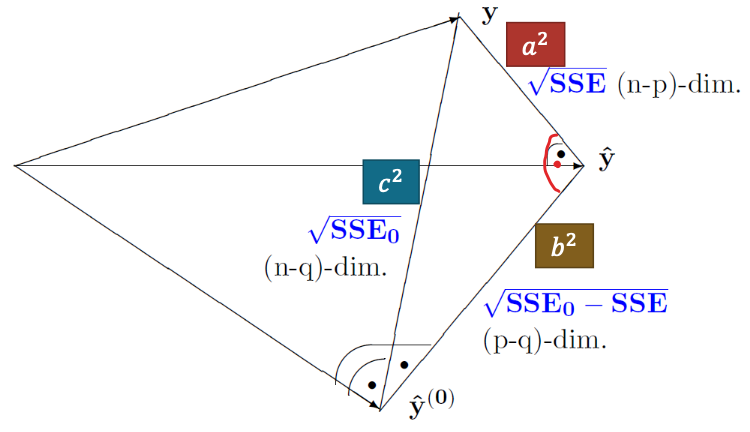
\includegraphics[width = 0.5\textwidth]{f_test_fig.png}
    \end{center}
\end{figure}

Under the assumption that the simple model is true, we have
\begin{equation*}
    \frac{\left(S S E_0-S S E\right) /(p-q)}{S S E /(n-p)}=\frac{\left\|\hat{\mathbf{Y}}-\widehat{\mathbf{Y}}^{(0)}\right\|^2 /(p-q)}{\|\mathbf{Y}-\widehat{\mathbf{Y}}\|^2 /(n-p)} \sim F_{p-q, n-p}
\end{equation*}

To show this, we use the following lemma which can be obtained using Lagrange multipliers:

\begin{lemma}{}{}
    The least squares estimator $\widehat{\mathbf{\beta}}_{(0)}$ under the supplementary condition $B \mathbf{\beta}=$ $\mathbf{b}$ is

    $$
    \widehat{\mathbf{\beta}}_{(0)}=\widehat{\mathbf{\beta}}-\left(X^T X\right)^{-1} B^T\left(B\left(X^T X\right)^{-1} B^T\right)^{-1}(B \widehat{\mathbf{\beta}}-\mathbf{b})
    $$

Furthermore,\footnote{To obtain this, one may use
$$
b^2=\left\|\hat{Y}-\hat{Y}_0\right\|^2=\left(X\left(\hat{\beta}-\hat{\beta}_0\right)\right)^T X\left(\hat{\beta}-\hat{\beta}_0\right)=\cdots
$$}
$$
\begin{gathered}
\underbrace{S S E_0}_{c^2}=\underbrace{S S E}_{a^2} + \underbrace{(B \widehat{\mathbf{\beta}}-\mathbf{b})^T\left(B\left(X^T X\right)^{-1} B^T\right)^{-1}(B \widehat{\mathbf{\beta}}-\mathbf{b}) .}_{b^2}
\end{gathered}
$$
\end{lemma}

We use this, and the fact $\hat{\sigma}^2 = \varepsilon^T \varepsilon / (n-p)$, to rewrite:
\begin{equation*}
    \frac{\left(S S E_0-S S E\right) /(p-q)}{S S E /(n-p)}=\frac{(B \widehat{\mathbf{\beta}}-\mathbf{b})^T\left(B\left(X^T X\right)^{-1} B^T\right)^{-1}(B \widehat{\mathbf{\beta}}-\mathbf{b})}{(p-q) \widehat{\sigma}^2} \sim F_{p-q, n-p}
\end{equation*}
One can show that this is a likelihood ratio test. We now show that this follows an $F$-distribution if $\epsilon \sim \mathcal{N}(0, \sigma^2 \mathbf{1})$.

\begin{proof}
    Recall that if $Y \sim \mathcal{N}(\mu, \Sigma)$, then $(y- \mu)^T \Sigma^{-1}(y-\mu) \sim \chi^2_n$. Also, $X = \frac{S_1 / d_1}{S_2 / d_2} \sim F_{d_1,d_2}$ if $S_i \sim \chi^2_{d_i}$ for $i = 1,2$ and $S_1 \perp S_2$.

    Since $\hat{\beta} \sim N(\beta, \sigma^2 (X^TX)^{-1})$,
    $$
    B \hat{\beta} \sim N(\underbrace{ B\beta }_{ =b }, \sigma^2B(X^TX)^{-1} B^T)
    $$

    Thus
    $$
    S_1 := (B \hat{\beta} - b)^T \left( \sigma^2 B (X^TX)^{-1} B^T \right)^{-1} (B \hat{\beta} - b) \sim \chi^2_{p-q}.
    $$
    We obtain the degrees of freedom by noting that $b$ is a $(p - q)$-dimensional vector.

    We have previously shown in Proposition \ref{prop:var_disr_n} (which relies on $\epsilon \sim \mathcal{N}(0, \sigma^2 \mathbf{1})$) that
    $$
    \frac{\sum_{ i=1 }^{ n } \hat{\varepsilon}_i^2 }{\sigma^2} \sim \chi^2_{n-p}
    $$
    A simple rearrangement, using $\hat{\sigma}^2 = \sum \hat{\varepsilon}_i^2 / (n-p) $  yields
    $$
    S_2 := \frac{(n-p) \hat{\sigma}^2}{\sigma^2} \sim \chi^2_{n-p}.
    $$
    Since $\hat{\varepsilon} \perp \hat{\beta}$, we have $S_1 \perp S_2$.

    Finally, after cancelling out some terms,
    $$
    \frac{S_1 / (p-q) }{S_2 / (n-p)} = \frac{(B \hat{\beta} - b)^T \left(  B (X^TX)^{-1} B^T \right)^{-1} (B \hat{\beta} - b)}{(p-q) \hat{\sigma}^2} \sim F_{p-q, n-p}.
    $$
\end{proof}

In R: Fit two nested models (e.g. fm and fm2) and compare with anova(fm, fm2).

\subsection{Residual Analysis}

Recall that errors are not identical to residuals. In particular,

\begin{itemize}
	\item \textbf{Errors}: $\varepsilon \sim N\left(0, \sigma^2 1\right) \rightarrow$ Errors are uncorrelated and have constant variance
	\item \textbf{Residuals}: $\hat{\varepsilon} \sim N\left(0, \sigma^2 M\right) \rightarrow$ Residuals are correlated and have different variance $\operatorname{Var}\left(\hat{\varepsilon}_i\right)=\sigma^2(1-$ $H_{i i}$ )
	\item By design: $\hat{y}$ and $\hat{\varepsilon}$ are uncorrelated
	\item We sometimes instead consider standardized residuals: $\hat{\varepsilon}_i^S=\frac{\hat{\varepsilon}_i}{\hat{\sigma} \sqrt{1-H_{i i}}} \rightarrow$ unit variance if the true model is correct.\footnote{If for instance $\operatorname{Var}(\epsilon) = \Sigma \neq \sigma^2 \mathbb{I}$, then the standardization will not yield a unit variance since we will not have $\hat{\varepsilon} \sim N\left(0, \sigma^2 M\right)$. We can spot this in adequate plots.}
\end{itemize}

There are four main assumptions to check:

\begin{enumerate}
    \item Independent samples:
    \begin{itemize}
        \item Plot residuals vs recording time or order of observation: is there serial correlation or clustering?
    \end{itemize}
    \item Functional relationship and constant variance
    \begin{itemize}
        \item Scatter plot $x -y $ in simple regression
        \item Tukey-Anscombe plot (residual vs fitted value $\hat{\varepsilon} - \hat{y}$)\footnote{Note: cannot be too picky with varying variances since residuals do not have constant variances.}
        \item Scale Location plot (standardised residual vs fitted value with horizontal smoother), see Figure \ref{fig:scale_loc}
    \end{itemize}
    \item Normal distribution of errors
    \begin{itemize}
        \item QQ-Plot of residuals
    \end{itemize}
\end{enumerate}


\begin{figure}
    \caption{Examples of scale-location plots. The left plot is okay, the right hand plot indicates problematic violations of assumptions as the variance seems to increase with the value of $\hat{y}$}
    \label{fig:scale_loc}
    \begin{center}
        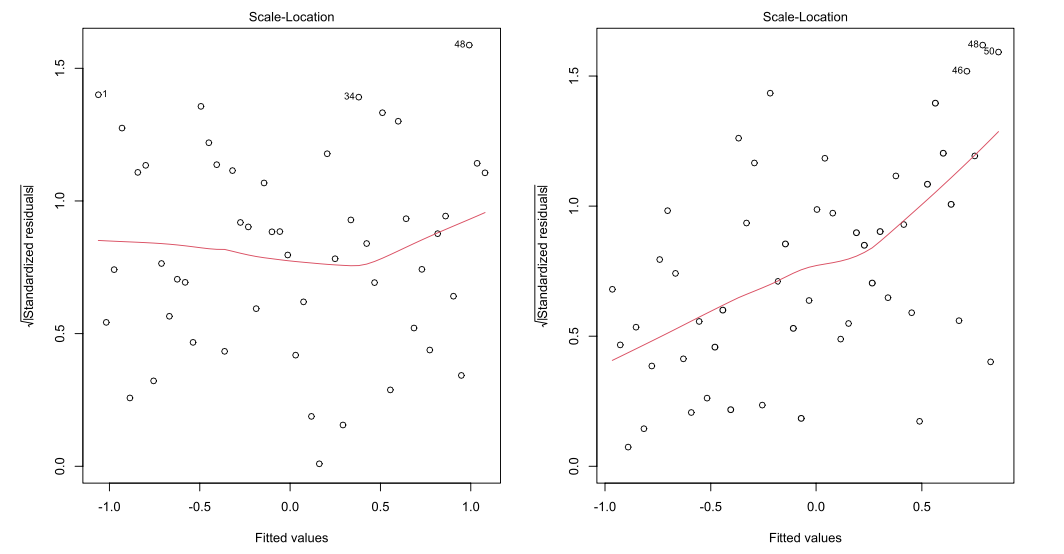
\includegraphics[width = 0.8\textwidth]{scale_location.png}
    \end{center}
\end{figure}

\subsubsection*{Outliers}

Outliers can occur in the $y$ or $x$ direction. Some ways of measuring outliers are:

\begin{itemize}
	\item \textbf{Leverage} $H_{i i}$: How influential is $y_i$ on prediction $\widehat{y}_i$?
	\begin{itemize}
		\item $\widehat{Y}=H Y \rightarrow \frac{d \widehat{y_i}}{d y_i}=H_{i i}$ depends on $X$ but not on $y$
	\end{itemize}
	\item \textbf{Cook's Distance} $\mathbf{D}_i$: How influential is $y_i$ on whole fit?
	\begin{itemize}
		\item Note: $\hat{y}_{j(i)}$ is the fitted response value for observation $j$ obtained when excluding observation $i$
		\item $D_i=\sum_{j=1}^n \frac{\left(\hat{y}_j-\hat{y}_{j(i)}\right)^2}{p \hat{\sigma}^2}$ can be transformed to $D_i=\frac{\hat{\varepsilon}_i{ }^2}{p \widehat{\sigma}^2} \cdot\left(\frac{H_{i i}}{\left(1-H_{i i}\right)^2}\right)$\footnote{Similarly, there is a transformation which can be applied to calculate LOOCV errors: $C V=\frac{1}{n} \sum_{i=1}^n \hat{\varepsilon}_{i(i)}^2$ can be transformed to $C V=\frac{1}{n} \sum_{i=1}^n\left(\frac{\hat{\varepsilon}_i}{1-H_{i i}}\right)^2$}
		\item Rule of thumb: $D_i>1$ is problematic
	\end{itemize}
\end{itemize}

We can investigate outliers in standard residual plots (e.g.,, residual vs leverage).


\section{Model Selection}

If we aim at \textbf{inference}, we should postulate one model as this allows for valid p-values.

If we instead explore multiple models, p-values etc. are no longer valid, we have a multiple testing issue. This is a research topic, post-selection inference.

Consequences of too many or too few variables in the model may be:
\begin{enumerate}
    \item \emph{Too few} (sparse model): Bias, but reduced variance\footnote{The model is unbiased if the missing variables are not correlated with the included $X$s. E.g., if we have a completely orthogonal design matrix.}
    \item \emph{Too many}: Unbiased, large variance
\end{enumerate}

In particular, overfitting is an issue which can reduce prediction accuracy when considering bigger models. This is the fundamental issue behind the bias-variance trade-off. We have
\begin{equation*}
    \text{MSE} = \operatorname{Var} + \operatorname{Bias}^2.
\end{equation*}


For this, note that when $z$ is an estimator of the unknown constant $c$,
$$
\begin{aligned}
    & E\left[(z-c)^2\right]=E\left[((z-E[z])+(E[z]-c))^2\right] \\
    & =\underbrace{E\left[(z-E(z))^2\right]}_{\operatorname{Var}(z)}+2 E\Big[\underbrace{(z-E[z])}_{\to 0} \cdot \underbrace{(E[z]-c)}_{\text { constant }}\Big]  +\underbrace{E\left[(E[z]-c)^2\right]}_{\text{bias}^2}
\end{aligned}
$$
Note that $E[z]-c$ is constant since we take expectation with respect to $z$, so $c$ is a constant and $E(E(z))$ is also just the expectation of a constant real number.

\subsection{Approaches for model selection}

\subsubsection*{Local approaches using F and t-tests}

Search strategies based on partial F-Test:

\begin{itemize}
	\item Stepwise forward
	\item Stepwise backward (only possible if $n>p$ )
	\item Add "most significant" / remove "least significant" variable according to partial F-test
\end{itemize}

Drawbacks:

\begin{itemize}
	\item p-values are used but not strictly valid anymore
	\item Only nested models can be compared
\end{itemize}

\subsubsection*{Global Approaches using Cp and AIC}

Often we do not want to use data splitting or cross-validation due to computational concerns. In this case, we can \textbf{estimate Test MSE} by using a formula that approximates the additional error in test MSE out-of-sample. That is, we want to minimize a quantitiy like
$$
\min RSS + c \cdot p
$$
where we have a penalty for complex models.


\begin{itemize}
    \item Mallow's $C_p$
    $$C_p=\frac{R S S}{\hat{\sigma}^2}+2|M|-n$$

    \item Akaike's Information Criterion:
    $$A I C=-2 \cdot l\left(\hat{\theta}_M\right)+2 \cdot p$$

    \item Bayesian Information Criterion:
    $$BIC=-2 \cdot l\left(\hat{\theta}_M\right)+\log (n) \cdot p$$
\end{itemize}

The last two criteria are more general than Mallow's $C_p$ as they are valid for all models which admit a likelihood.


\subsection{Derivation of Mallow's $C_p$}

We want to derive Mallow's $C_p$.

\textbf{Setup:}

\begin{itemize}
	\item Assume $y_i, i = 1, \dots, n$ independent.
	\item $\mathbb{E} \left[ y_i\right] = \mu_i, \operatorname{Var} \left( y_i\right) = \sigma^2$
	\item Regressors $1, x_1, \dots, x_k$ $\implies X$ is a $n \times (k+1)$ design matrix
	\item Consider a subset $M \subseteq \{ 0,1, \dots,k \}$, denote the design matrix of this reduced set of regressors by $X_M$ which is $n \times \left| M \right|$
\end{itemize}
Then
$$
\hat{\beta}_M = \left( x_M^T X_M \right)^{-1}  X_M^T y, \quad \hat{y}_M = X_M \hat{\beta}_M  = H_M y
$$

\textbf{Facts:}

\begin{enumerate}
	\item $E\left(\hat{Y}_M\right)=H_M E(y)=X_M\left(X_M^{\top} X_M\right)^{-1} X_M^{\top} X \beta$.
	\begin{itemize}
        \item Note that we may have bias as the $X_M$ and $X$ term do not cancel each other out
    \end{itemize}
	\item $\operatorname{Cov}\left(\hat{y}_M\right)=\sigma^2 H_M$
	\item $\sum_{i=1}^n \operatorname{Var}\left(\hat{Y}_{i M}\right)=\operatorname{tr}\left(\sigma^2 H_M\right)=\sigma^2 \operatorname{tr}\left(X_M\left(X^{\top} X_M\right)^{-1} X_M^{\top}\right)= \sigma^2 \left| M \right|$
	\item Sum of mean squared errors:\footnote{Note, this is a bit of a misnomer. Instead it is the sum of expected squared deviations between predictions and expected value for $y_i$.}

        Use $\mu_{iM} = \mathbb{E} \left[ \hat{y}_{iM}\right]$. Then

        \begin{equation}\label{eq:smse_rel}
            \begin{aligned}
                \text{SMSE}= & \sum_{i=1}^n \mathbb{E}\left[\left(\hat{y}_{i M}-\mu_i\right)^2\right] \\
                = & \sum_{i=1}^n E\left(\left(\hat{y}_{i M}-\mu_{i m}\right)+\left(\mu_{i m}-\mu_i\right)\right)^2 \\
                = & \sum \operatorname{Var}\left(\hat{y}_{i M}\right)+2 \sum E(\underbrace{\left(\hat{y}_{i M}-\mu_{i m}\right)}_{\rightarrow 0}\left(\mu_{i M}-\mu_i\right)) \\
                & +\sum \underbrace{ E\left(\mu_{i M}-\mu_i\right)^2 }_{ \text{constant, can remove }E }= \\
                = & \sigma^2|M|+\sum \left(\mu_{i M}-\mu_i\right)^2
                \end{aligned}
        \end{equation}

        We can then define
        \begin{equation}\label{gamma_cp}
            \gamma(M) = \frac{\text{SMSE}}{\sigma^2} = \left| M \right| + \frac{\text{bias}^2}{\sigma^2}
        \end{equation}
        We note that $\gamma(M) \geq M$ with equality if the model is unbiased.

	\item Future observations:

        Assume that we record again observations $y$ for all $i = 1, \dots, n$ with the same regressors $x_{i1}, \dots, x_{ik}$. Then
        $$
        Y_{n+i}=\mu_i+\underbrace{ \varepsilon_{n+i} }_{ \text{independent of} \varepsilon_1, \dots, \varepsilon_n }
        $$

        Since regressors are identical, our prediction $\hat{Y}_{n+i} = \hat{y}_n$.

        We define the \emph{expected squared prediction error (SPSE:)}\footnote{Note that we only consider squared errors on new observations.}
        \begin{equation}\label{eq:spse_rel}
            \begin{aligned}
                \text {SPSE}& = \sum_{i=1}^n \mathbb{E}\left[\left(Y_{n+i}-\hat{Y}_{i M}\right)^2\right] \\
                & =\sum E\left(\left(Y_{n+i}-\mu_i\right)-\left(\hat{Y}_{i m}-\mu_i\right)\right)^2 \\
                & =\sum(E\left(Y_{n+1}-\mu_i\right)^2-2 E\left(\underbrace{\left(Y_{n+i} - \mu_i\right) \left( \hat{Y}_{iM} - \mu_i \right) }_{\rightarrow 0}\right)+E\left(\hat{Y}_{i m}-\mu_i\right)^2) \\
                & =n \sigma^2+S M S E \\
                &=\underbrace{ n \sigma^2 }_{ (1) }+\underbrace{ |M| \sigma^2 }_{ (2) }+\underbrace{ \sum\left(\mu_{i M}-\mu_i\right)^2 }_{ (3) }
                \end{aligned}
        \end{equation}
        Note in the third line that $y_{n+i}$ and $\hat{y}_{iM}$ are independent. Therefore the expectation of the product is the product of expectations and we know that $E(Y_{n+i} - \mu_i) = 0$.

        We have the following three elements: (1) Irreducible error, (2) Variance, (3) Bias.
\end{enumerate}

Before deriving Mallow's $C_p$, we show the following relation:

\begin{lemma}{}{exp_rss}
    $$
    \mathbb{E} (\text {RSS})=\text { SPSE }-2|M| \sigma^2
    $$
\end{lemma}

For this, note that $\mathbb{E}(RSS)$ is the sum of expected squared residuals in sample (as opposed to SPSE which considers out of sample residuals).

\begin{proof}
    $$
    \begin{aligned}
    E(R S S)&=E\left(\sum\left(y_i-\hat{y}_i^M\right)^2\right)=\sum E\left(\left(y_i-\hat{y}_i^M\right)^2\right) \\
    & = \sum \underbrace{ \operatorname{Var}\left(y_i-\hat{y}_i^M\right) }_{ (1) }+\underbrace{ \sum\left(E\left(y_i-\hat{y}_i^M\right)\right)^2 }_{ (2) }
    \end{aligned}
    $$
    which follows from the usual formula for the variance, $\operatorname{Var}(X) = \mathbb{E}(X^2) - \left[\mathbb{E} (X) \right]^2$.

    \emph{ad (1):}

    $$
    \begin{aligned}
    & y-\hat{y}^M=y-H^M y=\left(\mathbf{1}-H^M\right) y \\
    & \operatorname{Cov}\left(\hat{y}-\hat{y}^M\right)=\left(\mathbf{1}-H^M\right) \sigma^2
    \end{aligned}
    $$
    Therefore,

    $$
    \begin{aligned}
    \begin{aligned}
    & \sum \operatorname{Var}\left(y_i-\hat{y}_i^M\right)=\sigma^2 \operatorname{tr}\left(\mathbf{1}-H^M\right) \\
    &= \sigma^2\left(n-\operatorname{tr}\left(H^M\right)\right)=\sigma^2(n-|M|)
    \end{aligned}
    \end{aligned}
    $$
    \emph{ad (2):}

    $$
    \begin{aligned}
    \sum\left(E\left(y_i-\hat{y}_i^M\right)\right)^2&=\sum\left(E\left(\hat{y}_i^M\right)-\mu_i\right)^2= \\
    &=  \text {SMSE}-|M| \sigma^2 \\
    &= \text{SPSE} -n \sigma^2-|M| \sigma^2
    \end{aligned}
    $$
    In the first step we use $\mathbb{E}(y_i) = \mu_i$. Then we used equations \eqref{eq:smse_rel}. In particular, we use $E(\hat{y}_{iM}) = \mu_{iM}$ and the last line in that block of equations. Finally, we use \eqref{eq:spse_rel} to get the result.

    Continuing with what we want to show, we have
    $$
    \begin{aligned}
    \mathbb{E} \left[ RSS\right]& =(n- | M| ) \sigma^2+S P S E- n \sigma^2-|M| \sigma^2= \\
    & =S P S E-2 \left| M \right| \sigma^2
    \end{aligned}
    $$
\end{proof}


Mallow's $C_p$ now wants to estimate $\gamma (M) = \frac{SMSE}{\sigma^2}$ as defined in \eqref{gamma_cp}. From the above,
$$
\begin{aligned}
\text { SPSE }&=n \sigma^2+S M S E=E(R S S)+2|M| \sigma^2  \\
 \Rightarrow & \text{ SMSE }=E(R S S)+2|M| \sigma^2-n \cdot \sigma^2
\end{aligned}
$$
We now replace unobserved aspects with estimates quantities,

$$
C_p=\frac{R S S}{\hat{\sigma}^2}+2|M|-n
$$


\subsection{Relation between $C_p$ and AIC for Linear Regression}

In linear regression,\footnote{Note that we have $|M| + 1$ parameters since we estimate $|M|$ coefficients and the residual standard error.}
$$
\mathrm{AIC}=-2 \cdot l\left(\hat{\beta}_M, \hat{\sigma}^2\right)+2(|M|+1)
$$
The term of the log-likelihood is given by
$$
\begin{aligned}
-2 l\left(\hat{\mathbf{\beta}}_M, \hat{\sigma}^2\right) & =n \log \left(\hat{\sigma}^2\right)+\frac{1}{\hat{\sigma}^2}\left(\mathbf{y}-\mathbf{X}_M \hat{\mathbf{\beta}}_M\right)^{\prime}\left(\mathbf{y}-\mathbf{X}_M \hat{\mathbf{\beta}}_M\right) \\
& =n \log \left(\hat{\sigma}^2\right)+\frac{n \hat{\sigma}^2}{\hat{\sigma}^2} \\
& =n \log \left(\hat{\sigma}^2\right)+n.
\end{aligned}
$$
We get
\begin{equation}\label{eq.aiclinreg}
    \mathrm{AIC}=n \cdot \log \left(\hat{\sigma}^2\right)+2(|M|+1) + n
\end{equation}
This looks quite different to $C_p$, but we can show similarity by applying a Taylor expansion of $\log \hat{\sigma}^2$ around $\sigma^2$ to obtain
$$
\log \hat{\sigma}^2 \approx \log \sigma^2 + \frac{1}{\sigma^2} \left(\hat{\sigma}^2-\sigma^2\right) = \log \sigma^2 + \frac{SSE}{n \sigma^2} -1
$$

Thus, ignoring the constant $2+n$ in \eqref{eq.aiclinreg},
$$
AIC \approx n \log \left(\sigma^2\right)+\underbrace{ \frac{S S E}{\sigma^2}-n+2 \left| M \right|  }_{ \approx C_p }
$$



\subsection{General Search Strategies}

\begin{itemize}
	\item \textbf{Exhaustive Search}
	\begin{itemize}
		\item For given $p=1, \ldots, p_{\text {max }}$: Find best model according to RSS\footnote{We do not require an information criteria for a fixed number of parameters $p$ since in this case the model with lowest RSS automatically has the lowest value for the information criteria.}
		\item We obtain $p_{\text {max }}$ different models
		\item We then choose the best one with $\mathrm{C}_p$ or $\mathrm{AIC}$,
		\begin{itemize}
			\item Pros: Finds global optimum
			\item Cons: Computational cost $p$ variables $\rightarrow 2^p$ subsets
		\end{itemize}
	\end{itemize}
	\item \textbf{Forward / Backward Selection}
	\begin{itemize}
		\item Forward: Start with empty model, add one variable at a time
		\item Backward: Start with full model, remove one variable at a time
		\item E.g., in forward selection we calculate $C_p$ for each potential $p^\prime +1$ variable model with first $p$ variables fixed after having found best $p^\prime$ model. If there is no model with a better $C_p$ value, we stop.\footnote{The R implementation in regsubsets finds the best model according to RSS for any potential number of variables and only in the end chooses according to information criteria between models with different number of parameters.}
		\begin{itemize}
            \item Pros: Fast
		    \item Cons: Only local optimum $\rightarrow$ Forward and Backward often get to different final models
        \end{itemize}
	\end{itemize}
\end{itemize}

In R:

\begin{lstlisting}
regsubsets(y ~ ., data, method = "exhaustive", nvmax = 15)
\end{lstlisting}



\section{Non i.i.d. errors}

Assume $\operatorname{Cov} \left( \varepsilon \right) = \sigma^2 \mathbb{I}$. Then we can show that
$$
\operatorname{Cov} \left( \hat{\beta}\right) =  \sigma^2 (X^T X)^{-1}
$$
Now, instead assume $\operatorname{Cov} \left( \varepsilon\right) = \sigma^2 W^{-1}$. Then
$$
\operatorname{Cov} \left( \hat{\beta}\right) =\sigma^2 (X^T X)^{-1} X^T W^{-1} X (X^T X)^{-1} \neq \sigma^2 (X^T X)^{-1}
$$
$\implies$ Using 'normal' OLS leads to wrong p-values and CIs.

Often times we can detect deviations from $\operatorname{Cov} \left( \varepsilon \right) = \sigma^2 \mathbb{I}$ by investigating TA-plots or from context knowledge (e.g., grouped measurements). In particular if we have additional information about the form of the covariance matrix, we can often use such information to estimate the covariance matrix and obtain correct CIs.


\subsection{Known covariance matrix -- Generalised Least Squares}

Suppose we know the covariance matrix of our errors up to a factor. E.g.,
\begin{equation*}
    \mathbf{Y}=X \mathbf{\beta}+\mathbf{\varepsilon} \quad \varepsilon \sim \mathcal{N}\left(\mathbf{0}, \sigma^2 \Sigma\right)
\end{equation*}
where $\Sigma$ is known and PD. By Proposition \ref{prop:sqrt_matrix} (and due to PD, thus invertibility), there exists an invertible matrix $A$ such that
\begin{equation*}
    \Sigma^{-1} = (A A^T)^{-1}
\end{equation*}

We can thus formulate our OLS problem in a `tilde' dimension where we use
\begin{equation*}
    \tilde{\mathbf{Y}}:=A^{-1} \mathbf{Y}=A^{-1}(X \beta+\mathbf{\varepsilon})=\underbrace{A^{-1} X}_{\tilde{X}} \mathbf{\beta}+\underbrace{A^{-1} \mathbf{\varepsilon}}_{\tilde{\varepsilon}}=\tilde{X} \mathbf{\beta}+\tilde{\mathbf{\varepsilon}}
\end{equation*}

We have
\begin{align*}
        \mathbb{E} \tilde{\varepsilon} & =\mathbb{E} A^{-1} \varepsilon=A^{-1} \mathbb{E} \varepsilon=\mathbf{0} \\
        \operatorname{Cov}[\tilde{\varepsilon}] & =\operatorname{Cov}\left[A^{-1} \varepsilon\right]=A^{-1} \operatorname{Cov}[\varepsilon]\left(A^{-1}\right)^T \\
        & =A^{-1} \sigma^2\left(A A^T\right)\left(A^{-1}\right)^T=\sigma^2 I .
\end{align*}

We can thus apply our usual OLS results to estimate $\hat{\beta}$ from the `tilde model'
\begin{equation*}
    \|\tilde{\mathbf{Y}}-\tilde{X} \mathbf{\beta}\|^2=(\mathbf{Y}-X \mathbf{\beta})^T A^{-T} A^{-1}(\mathbf{Y}-X \mathbf{\beta})=(\mathbf{Y}-X \mathbf{\beta})^T \Sigma^{-1}(\mathbf{Y}-X \mathbf{\beta}).
\end{equation*}
We can think of this as rescaling our residuals such that observations with larger variance (more uncertainty) receive a lower weight. This will be more obvious in the special case where $\Sigma$ is diagonal which we treat below.

Solving the above for $\hat{\beta}$ gives us our usual result in the tilde dimension:
 \begin{equation*}
    \widehat{\mathbf{\beta}}=\left(\tilde{X}^T \tilde{X}\right)^{-1} \tilde{X}^T \tilde{\mathbf{Y}}=\left(X^T \Sigma^{-1} X\right)^{-1} X^T \Sigma^{-1} \mathbf{Y}.
 \end{equation*}

 In the last step we plug back in our definitions of $\tilde{X}, \tilde{Y}$. It is then easy to see that
 \begin{equation*}
    \widehat{\mathbf{\beta}} \sim \mathcal{N}_p\left(\mathbf{\beta}, \sigma^2\left(X^T \Sigma^{-1} X\right)^{-1}\right), \quad \hat{\sigma}^2=\frac{1}{n-p} \varepsilon^T \Sigma^{-1} \varepsilon
 \end{equation*}

 If we know that each $y_i$ is an average of $w_i$-many i.i.d. measurements, we obtain the special case of \textbf{weighted least squares.}

 \begin{equation*}
    \operatorname{Var}\left(\varepsilon_i\right)=\frac{\sigma^2}{w_i} ; \quad \operatorname{Cov}(\varepsilon)=\sigma^2 \operatorname{diag}\left(\frac{1}{w_1}, \ldots, \frac{1}{w_n}\right)=\sigma^2 \Sigma
 \end{equation*}
 Thus
 \begin{align*}
    |\tilde{Y}-\tilde{X} \beta|^2&= \left[A^{-1}(Y-X \beta)\right]^T A^{-1} \left[Y-X \beta\right] \\
    &=(Y-X \beta)^T \Sigma^{-1}(Y-X \beta)=\sum_{i=1}^n w_i\left(y_i-x_i^T \beta\right)^2
 \end{align*}
 Each observation in our objective function is weighted proportionally to the \textbf{number of samples} or \textbf{inverse variance of error}. Note that WLS in general encapsulates cases where we have heteroskedastic but uncorrelated errors and know the heteroskedasticity strucutre. In this case, we have $\Sigma^{-1} = W^{1/2} W^{1/2}$ where $W = \operatorname{diag}(w_1, \ldots, w_n)$, so $A^{-1} = A^{-\top} = W^{1/2}$.

 In R: \lstinline|fm <- lm(y ~ x, data = df, weights = nreps)|, weights arugment

 From the fact that we can rescale our model to a tilde dimension with diagonal covariance matrix, we can apply many of our previous results, in particular:

\begin{proposition}{Gauss-Markov for WLS}{}
    Among all linear and unbiased estimators $\hat{\mathbf{\beta}}^L=$ $\mathbf{A} \mathbf{y}$, the WLS estimator has minimal variance, i.e.,
    $$
    \operatorname{Var}\left(\hat{\beta}_j\right) \leq \operatorname{Var}\left(\hat{\beta}_j^L\right), \quad j=0, \ldots, k
    $$
\end{proposition}

A similar extension holds with normally distributed errors and WLS being the minimal variance unbiased estimator.

Note that we could use our normal OLS estimate and the fact that
$$
\operatorname{Var}(\hat{\beta}_\text{OLS}) = \sigma^2 (X^T X)^{-1} X^T \Sigma X (X^T X)^{-1}
$$
while plugging in $\Sigma$ to obtain correct coverage probabilities. However, the above application of the Gauss-Markov theorem shows that instead using Generalized Least Squares leads to more efficient estimates.

 \subsection{Unknown covariance matrix, known structure}

 \subsubsection*{MLE and two-stage OLS}

If our covariance matrix is unknown, but we can specify the structure, we can usually use this information to model the covariance matrix. There are two approaches:

\begin{enumerate}
    \item Two-stage procedure
    \begin{enumerate}
        \item Fit OLS
        \item Use OLS residual estimates and information about Covariance structure to model coefficients of covariance
        \item Use above to derive weights and fit GLS
        \item Iterate
        \item Example: Serial correlation of AR(1) form
        \begin{equation*}
            \operatorname{Cov}(\varepsilon)=\sigma^2 W^{-1}=\frac{\sigma_u^2}{1-\rho^2}\left(\begin{array}{ccccc}
                1 & \rho & \rho^2 & \cdots & \rho^{n-1} \\
                \rho & 1 & \rho & \cdots & \rho^{n-2} \\
                \vdots & \vdots & \vdots & \ddots & \vdots \\
                \rho^{n-1} & \rho^{n-2} & \rho^{n-3} & \cdots & 1
                \end{array}\right)
        \end{equation*}
        We estimate residuals using OLS, then estimate $\rho_1, ..., \rho_k$ using residuals and use $\rho$ to define weights to be used in GLS.
    \end{enumerate}
    \item Maximum-Likelihood
    \begin{enumerate}
        \item Make assumption about distribution of $\varepsilon$ and write out likelihood using known information about covariance matrix
        \item Estimate covariance matrix using MLE
    \end{enumerate}
\end{enumerate}


\subsubsection*{Huber-White HC (Sandwich) Estimator}

Consider the model
$$
\begin{aligned}
& Y=X \beta+\varepsilon, \varepsilon \sim \mathcal{N}_n(0, D) \\
& D=\operatorname{diag}\left(\sigma_1^2, \ldots, \sigma_n^2\right), \sigma_i^2=\operatorname{Var}\left(\varepsilon_i\right).
\end{aligned}
$$

We know that
$$
\hat{\beta} \sim \mathcal{N}_p\left(\beta,\left(X^T X\right)^{-1} X^T D X\left(X^T X\right)^{-1}\right).
$$

For statistical testing or confidence intervals, we need to estimate the covariance matrix. An easy but powerful approach is to use
$$
\hat{D}=\operatorname{diag}\left(r_1^2, \ldots, r_n^2\right)
$$
where $r=Y-X \hat{\beta}$ are the residuals (from the least squares estimator). The estimated covariance matrix is then
$$
\hat{V} = \left.\widehat{\operatorname{Cov}}(\hat{\beta})=\left(X^T X\right)^{-1} X^T \hat{D} X\left(X^T X\right)^{-1}\right) .
$$

Note that it may seem implausible to estimate this, as we have $n$ observation and the matrix $\hat{D}$ consists of $n$ parameters. However, we can show that we can estimate the term $X^T \hat{D} X$ consistently. In particular, since we know $V^{-1 / 2}(\hat{\beta}-\beta) \sim \mathcal{N}_p(0, I)$, we now want to show:
\begin{equation*}
    \hat{V}^{-1 / 2}(\hat{\beta}-\beta) \Longrightarrow \mathcal{N}_p(0, I) \; \text{ as }n \rightarrow \infty
\end{equation*}
It follows from Slutsky's theorem (Theorem \ref{thm:slutsky}) that this is the case if we can consistently estimate $V$.\footnote{Normality of $V^{-1 / 2}(\hat{\beta}-\beta)$ follows from our usual arguments of either the distribution of $\epsilon$ or a central limit theorem. The part of interest is now whether we can replace $V^{-1 / 2}$ with our estimated covariance matrix $\hat{V}^{-1 / 2}$.}  Thus, we want to show that $\hat{\beta} \overset{p}{\to} \beta \text{ as } n \to \infty$ and
\begin{equation}\label{eq:51}
    n(\widehat{\operatorname{Cov}}(\hat{\beta})-\operatorname{Cov}(\hat{\beta})) \rightarrow 0
\end{equation}
We multiply by $n$ since Slutsky's theorem requires sufficiently fast convergence of $\hat{V} \to V$. Since $\operatorname{Cov}(\hat{\beta})$ itself shrinks at $n^{-1}$, we must have convergence of $\hat{V} \to V$ at a faster rate which we ensure by checking whether $n(\hat{V}  -V) \to 0$.


\begin{lemma}{}{converge_b_prob}
    Assume $D$ diagonal and $Y = X \beta + \varepsilon$ with $\varepsilon \sim \mathcal{N}(0, D)$. Let $\hat{\beta} = (X^T X)^{-1} X^T y$. Estimate $\hat{D} = \operatorname{diag}(\hat{\varepsilon}_1^2, \ldots, \hat{\varepsilon}_n^2)$. Assume further that
    \begin{enumerate}
        \item $ \frac{X^T X}{n} \to C$ as $n \to \infty$ where $C$ is psd
        \item $\sigma^2_i < C_1 < \infty$ for all $i$, and $1/n \sum X_{ij}^2 \leq C_2 < \infty$ for all $j$
    \end{enumerate}

    Then
    \begin{equation*}
        \hat{\beta} \overset{p}{\to} \beta \text{ as } n \to \infty
    \end{equation*}
\end{lemma}

\begin{proof}
    We know that our estmated $\hat{\beta}$ is unbiased. We therefore only need to show that the covariance converges to 0.

    We write
    $$
    \operatorname{Cov} \left( \hat{\beta}\right) = \frac{1}{n} \left( \underbrace{ \frac{X^TX}{n}}_{ (1) } \right)^{-1} \underbrace{ \frac{X^TD X}{n}  }_{ (2) }\underbrace{ \left( \frac{X^TX}{n} \right)^{-1} }_{ (3) }.
    $$

    We know that terms $(1)$ and $(3)$ are bounded by assumption 1. Further, term $(2)$ is bounded by assumption 2 since any element of $\dfrac{X^T D X}{n}$ is weakly smaller than $C_1 \cdot C_2$.  Therefore,
    $$
    \operatorname{Var} \left( \hat{\beta_j}\right) \to 0 \text{ as } n \to \infty, \;\forall j.
    $$

    By Tchebshev's inequality,
    $$
    \lim_{ n \to \infty } P \left( \left| \hat{\beta}_j - \beta_j \right| > \varepsilon  \right) = 0, \;\forall \varepsilon > 0
    $$
\end{proof}

\begin{lemma}{}{}
    In addition, assume $\max_{i,j} |X_{ij}| \leq K <\infty$. Then
    \begin{equation*}
        \frac{X^T \hat{D} X}{n} - \frac{X^T D X}{n} \overset{p}{\to} 0 \text{ as } n \to \infty
    \end{equation*}
\end{lemma}

\begin{proof}
    Consider an arbitrary elements $(r,s)$. We can write
    \begin{equation}\label{eq_def_xtdx_sum}
        \frac{1}{n} \left( X^T \hat{D} X \right)_{rs} = \frac{1}{n} \sum_i X_{ir} X_{is} \hat{\varepsilon}_i^2
    \end{equation}
    Then,
    $$
    \begin{aligned}
    \frac{1}{n} \left( X^T \hat{D} X \right)_{rs} &= \frac{1}{n} \sum_i X_{ir} X_{is} \hat{\varepsilon}_i^2 \\
    &= \frac{1}{n} \sum X_{ir} X_{is} \left( y_i - \hat{y}_i \right)^2 \\
    &= \frac{1}{n} \sum X_{ir} X_{is} \left( \varepsilon_i - \underbrace{ x_i^T (\hat{\beta}- \beta) }_{ \to 0 } \right)^2 \\
    &= \frac{1}{n} \sum X_{ir} X_{is} \left(  \varepsilon_i^2 + o_p(1) \right)
    \end{aligned}
    $$
    In the second last line we use our above result that $\hat{\beta} \to \beta$ in probability as $n \to \infty$.

    To show consistency, we first show asymptotic unbiasedness.
    $$
    \mathbb{E} \left[ \frac{1}{n} \sum X_{ir} X_{is}  \varepsilon_i^2 \right] = \frac{1}{n} \sum X_{ir} X_{is}  \sigma^2_i = \frac{1}{n} (X^T D X)_{rs}
    $$
    where we use \eqref{eq_def_xtdx_sum} for population values (and in reverse).

    Next, we show that the variance converges to $0$ as $n \to \infty$,
    $$
    \begin{aligned}
    \operatorname{Var} \left(  \frac{1}{n} \sum X_{ir} X_{is}  \varepsilon_i^2 \right) &= \frac{1}{n} \frac{1}{n} \sum_{i = 1}^n X_{ir}^2 X_{is}^2  \operatorname{Var} \left( \varepsilon_i^2\right)\\
    &= \frac{1}{n} \frac{1}{n} n \cdot \text{constant} \to 0 \; (n \to p)
    \end{aligned}
    $$
    For this, we may use that if $\varepsilon_i \sim \mathcal{N}(0, \sigma^2_i)$ then $\operatorname{Var} \left( \varepsilon_i^2\right) = 3 \sigma^4_i < \infty$.

    Thus, $\frac{X^T \hat{D} X}{n} - \frac{X^T D X}{n} \overset{p}{\to} 0 \text{ as } n \to \infty$.
\end{proof}

This allows us to proof \eqref{eq:51} since
$$
n \left[\widehat{\operatorname{Cov}} \left( \hat{\beta}\right) -  \operatorname{Cov} \left( \hat{\beta}\right) \right] = \left(  \frac{X^TX}{n} \right)^{-1} \left[ \frac{X^T \hat{D} X}{n} - \frac{X^T D X}{n}\right] \left( \frac{X^TX}{n} \right)^{-1}
$$
where the mid term converges to zero and the other terms converge to some constant matrix $C$.

What is the risk that we ``badly'' estimate at least one element of the matrix if we also allow the number of covariates to grow? We can upper-bound this error by $p^2 \sup \operatorname{Pr}\left(\text {error}_i\right)$. Note that the probabiltiy of an error goes down at rate $n^{-1}$, as shown. If the number of covariates $p$ grows at a smaller rate, e.g., $\log N$, this error probabiltiy still converges to 0.



One fundamental application of the HC estimator is when using linear models to approximate complex models. Even if we have $Y_i = f(X_i) + \varepsilon_i$ with $\varepsilon_i$ independent of $X_i$, and $\operatorname{Var}(\varepsilon_i) = \sigma^2$  when we use a linear approximation, we will have a heteroskedastic error.

In R: \lstinline|coeftest(fm, vcov = vcovHC(fm, type = "HC0")| from sandwhich package.


\subsection{Mixed Models}

Another approach of modelling more complex error structures is to use mixed models. Suppose we have $i$ individuals or clusters, and $n_i$ observations per individual. Coefficients are likely to be different across people. One approach would be to have a block factor:

\begin{equation*}
    y_{i j}=\left(\beta_0+\beta_{0, i}\right)+\beta_1 x_j+\varepsilon_{i j}, \quad \varepsilon_{i j} \sim N\left(0, \sigma^2\right) i . i . d
\end{equation*}

Here we only consider \emph{fixed effects} and include a custom level-shift per cluster. With this we can easily make statements about individual intercepts but less easily derive statements about the underlying distribution.

A different approach uses so called random effects.

\subsubsection*{Random Intercept Model}

\begin{align*}
    y_{i j}&=\left(\beta_0+u_i\right)+\beta_1 x_{i j}+\varepsilon_{i j}, \\
    \varepsilon_{i j} &\sim N\left(0, \sigma^2\right), \; u_i \sim N\left(0, \sigma_1^2\right) \; \text { i.i.d } \\
    \varepsilon_{ij} &\perp u_k, \forall i, j, k
\end{align*}
I.e., we have a cluster-specific random shift ($u_i$).

This is a \textbf{mixed model} since we consider both fixed and random effects. We can easily study statements about the dispersion of of initial slopes in the population but not about indvidiuals.

It turns out that we implicitly model the correlation among samples of the same cluster.

Within block $i$:
$$
    \begin{aligned}
    \operatorname{Cov} \left( Y_{ij}, Y_{ik}\right) &= \operatorname{Cov} \left( u_i + \varepsilon_{ij}, u_k + \varepsilon_{ik}\right) \\
    &=\operatorname{Cov} \left( u_i, u_k\right) + \operatorname{Cov} \left( \varepsilon_{ij}, \varepsilon_{ik}\right) \\
    &=\sigma^2_1 + \sigma^2 \mathbf{1} \{ j = k \}
    \end{aligned}
$$

Between blocks, we have zero covariance. Let $m \neq i$,
\begin{equation*}
    \operatorname{Cov}\left(Y_{i j}, Y_{m k}\right)=\underbrace{\operatorname{Cov}\left(\mu_i, \mu_m\right)}_{=0}+\underbrace{\operatorname{Cov}\left(\varepsilon_{i j}, \varepsilon_{m k}\right)}_{=0}
\end{equation*}
We therefore obtain a block-diagonal covariance matrix.
\begin{itemize}
    \item Constant correlation structure
    \item Relative strength of within-subject correlation depends on relative magnitudes of $\sigma^2$ and $\sigma^2_1$
\end{itemize}


\subsubsection*{Random Intercept Random Slope Model}

We can naturally extend this model to allow for variying slopes between clusters. We now not only consider a random shift in the intercept but also a random shift for the slope parameter.

\begin{equation*}
    \begin{aligned}
        & y_{i j}=\left(\beta_0+u_{1, i}\right)+\left(\beta_1+u_{2, i}\right) x_{i j}+\varepsilon_{i j}, \\
        & \varepsilon_{i j} \sim N\left(0, \sigma^2\right) i . i . d \\
        & u_{1, i} \sim N\left(0, \sigma_1^2\right), \\
        & u_{2, i} \sim N\left(0, \sigma_2^2\right), \\
        & \operatorname{cor}\left(u_1, u_2\right)=\rho
        \end{aligned}
\end{equation*}

We initially estimate models using MLE to compare models. To obtain the final model we use restricted MLE (RMLE), as this removes the biased estimation of standard deviations.\footnote{We initially use MLE due to better properties of MLE and allowing comparison of non-nested models.}

Note: The standard deviation of our slope and intercept estimates will approach the population values as $n \to \infty$, however, the standard error of the estimates will go to $0$.


In R: \lstinline|lmer| function in lme4 library.

\subsubsection*{Comparing Fixed Effects and Random Effects}

Note that the question of fixed vs random effects depends fundamentaly on the question one wants to answer. If one is interested in the specific sample, fixed effects are more useful, while random effects allow inference about population attributes.

In terms of estimation, fixed effects are modelled by explicitly including a dummy variable for each cluster in the design matrix $X$ and estimating coefficients for each cluster, e.g., $\alpha_i$, throuhg OLS. On the other hand, to estimate random effects we use MLE and specify that the random effects follow a normal distribution from which we then find $\hat{\sigma}^2_1$.\footnote{Some libraries such as lme4 can still extract actual random effects by using a technique called \emph{best linear unbiased prediction (BLUP)}. After estimating $\hat{\sigma}^2_1$, BLUPs are calculated for each random effect by taking conditional expectations of random effects given data and estimated coefficietns. The formula in a RI model is given by:
\begin{equation*}
    \hat{b}_j=\frac{\sigma_1^2}{\sigma_1^2+\sigma^2 / n_j}\left(\bar{y}_j-\beta_0-\beta_1 \bar{x}_j\right)
\end{equation*}
I.e., instead of estimating each coefficient directly, we estimate distribution parameters and then obtain random effects by taking conditional expectations.
}
Since we estimate fewer parameters, this allows scaling to larger number of random effects.


\subsubsection*{General Linear Mixed Models}

We can greatly increase complexity of such models by having more complicated random effects and more complex covariance structures. This gives rise to \emph{General Linear Mixed Models}.

Consider $y_i$ to be an $n$-dimensional vector for cluster $i$:
\begin{equation*}
    \begin{aligned}
        & y_i=x_i \beta+u_i \gamma_i+\varepsilon_i \\
        & \gamma_i \sim \mathcal{N}(0, Q), \quad \varepsilon_i \sim \mathcal{N}\left(0, \sigma^2 \Sigma_{n_i}\right), \quad \gamma_i, \varepsilon_i \text { indep. }
        \end{aligned}
\end{equation*}
We obtain the \emph{conditional formulation} of our model by conditioning on random effects (i.e., we fix cluster $i$):
\begin{equation*}
    y_i \mid \gamma_i \sim \mathcal{N}\left(x_i \beta+u_i \gamma_i, \sigma^2 \Sigma_{n_i}\right)
\end{equation*}
The \emph{marginal formulation} subsums random effects and other noise terms:
 \begin{equation*}
    \begin{aligned}
        & y_i=X_i \beta+\varepsilon_i^*; \quad E\left(y_i\right)=X_i \beta \\
        & \operatorname{Cov}\left(y_i\right)=\operatorname{Cov}\left(u_i \gamma_i\right)+\operatorname{Cov}\left(\varepsilon_i\right)= u_i Q u_i^{\top}+\sigma^2 \Sigma_{n_i} \\
        & \Rightarrow Y_i \sim \mathcal{N}\left(x_i \beta, \sigma^2 \Sigma_{n_i}+u_i Q u_i^{\top}\right)
    \end{aligned}
 \end{equation*}

 \begin{example}{}{}
    To recover the RI model from the above, use
	\begin{equation*}
		u_i=(1, \ldots, 1)^{\top}, \;Q=\sigma_1^2, \; \Sigma=\mathbb{I}
	\end{equation*}
     We would then recover the exact same structure we had above.
\end{example}

Residual analysis is more difficult, as the complicated error structure leads to many technicalities. We can investigate Turkey-Anscombe plots but should only consider major deviations. We can also use QQ-plots on the estimated random effects to investigate whether the normality assumption holds.

To summarise: A general linear mixed model is given by
$$
y=X \beta+U \gamma+\varepsilon
$$
with
$$
\binom{\gamma}{\varepsilon} \sim N\left(\binom{0}{0},\left(\begin{array}{ll}
G & 0 \\
0 & R
\end{array}\right)\right) .
$$
In this model, $\mathbf{X}$ and $\mathbf{U}$ are design matrices, $\mathbf{\beta}$ is a vector of fixed effects, and $\gamma$ is a vector of random effects. The covariance matrices for $\gamma$ and $\mathbf{\varepsilon}$ are assumed to be nonsingular, and therefore positive definite, and $\gamma$ and $\varepsilon$ are independent.

\begin{equation*}
    \mathbf{U}=\operatorname{blockdiag}\left(\mathbf{U}_1, \ldots, \mathbf{U}_i, \ldots, \mathbf{U}_m\right)=
    \begin{bmatrix}
        \mathbf{U}_1 & & & & \mathbf{0} \\
        & \ddots & & & \\
        & & \mathbf{U}_i & & \\
        & & & \ddots & \\
        \mathbf{0}& & & & \mathbf{U}_m
    \end{bmatrix}
\end{equation*}

$\mathbf{\varepsilon} \sim N (\mathbf{0}, \mathbf{R}), \mathbf{\gamma} \sim N(\mathbf{0}, \mathbf{G})$ with block diagonal covariance matrices:
\begin{align*}
    & \mathbf{R}=\operatorname{blockdiag}\left(\sigma^2 \mathbf{\Sigma}_{n_1}, \ldots, \sigma^2 \mathbf{\Sigma}_{n_i}, \ldots, \sigma^2 \mathbf{\Sigma}_{n_m}\right) \\
    & \mathbf{G}=\operatorname{blockdiag}(\mathbf{Q}, \ldots, \mathbf{Q}, \ldots, \mathbf{Q})
\end{align*}

Note: dimensions of above elements
\begin{itemize}
	\item $\boldsymbol{y}_i$ is an $n_i \times 1$ response vector.
	\item $\boldsymbol{X}_i$ is an $n_i \times p$ fixed-effects design matrix.
	\item $\boldsymbol{\beta}$ is a $p \times 1$ vector of fixed-effect coefficients (common across groups).
	\item $\boldsymbol{U}_i$ is an $n_i \times q_i$ random-effects design matrix. E.g., this could consist of one column of ones and one column with time observations in a typical RIRS example.
	\item $\boldsymbol{\gamma}_i$ is a $q_i \times 1$ vector of random-effect coefficients. E.g., we assume that there is some randomness in initial reaction time and response to days of sleep deprivation between people. $\boldsymbol{\gamma}_i$ is the ``drawn'' value from this random distribution which specifies initial reaction and reaction to sleep deprivation for individual $i$.
	\item $\varepsilon_i$ is an $n_i \times 1$ vector of random errors.
\end{itemize}


\subsection{Comparison between different approaches for non iid errors}

\begin{itemize}
    \item Generalised Least Squares:
    \begin{itemize}
        \item applicable to heteroskedastic and correlated erros but requires knowledge of covariance matrix up to multiplicative factor.
        \item Different coefficient estimates.
    \end{itemize}
    \item Two-stage or MLE:
    \begin{itemize}
        \item applicable to heteroskedastic and correlated erros but requires a parametric form of covariance structure (e.g., AR process) (do not require exact covariance matrix ex ante).
        \item Different coefficient estimates.
    \end{itemize}
    \item Huber-White:
    \begin{itemize}
        \item Applicable to heteroskedastic but uncorrelated errors.
        \item Note: same coefficient estimates as OLS
        \item Heteroskedasticity and autocorrelation robust estimators exist.
    \end{itemize}
    \item Mixed-models:
    \begin{itemize}
        \item Implicitly models error structure through random effect structure, can include both heteroskedastic and correlated errors but requires knowledge of grouping of data.
        \item Different coefficient estimates.
        \item Higher variance compared to other approaches but less detailed knowledge about covariance matrix required.
    \end{itemize}
\end{itemize}


\clearpage


\section{Generalized Linear Models}

\textbf{Generalized Linear Models (GLMs)} model relationships between explanatory variables and the parameter of the distribution. That is, we assume our target variable follows some distribution $F(\theta(X))$ whose parameters depend on $X$.
\begin{equation*}
    \begin{aligned}
        S:& \quad Y \sim F(\theta(X)) \\
        D:& \quad  g \big(\theta(X)  \big)= \beta_0 + \beta_1 x
    \end{aligned}
\end{equation*}
Note that while $Y$ is stochastic, we view the link between the parameter and our covariates as being deterministic (no error term).\footnote{I.e., we do not explicitly include or model an error term $\varepsilon$. Previously, randomness in $Y \mid X$ only depended on the error, we now instead model $Y$ to follow the distribution $F(\theta(X))$ directly.}

Three key components:
\begin{itemize}
    \item Link function $g(\cdot)$
    \item Linear (in $\beta$) predictor
    \item Distribution of $Y$
\end{itemize}

We will see that GLM usually assumes that
\begin{itemize}
    \item $F(\theta)$ is in exponential family
    \item $\theta$ is expected value
    \item Every  $F(\theta)$ then has a canonical link function with `nice' properties
\end{itemize}

\begin{example}{Linear Regression as GLM}{}
    Linear regression is a special case of GLM where we model $Y$ to be normally distributed, with the mean depending on $X$.
    \begin{align*}
            & \mathrm{S}: Y \sim N\left(\mu(x), \sigma^2\right) \\
            & \mathrm{D}: \mu(x)=\beta_0+\beta_1 x
    \end{align*}
\end{example}

\begin{example}{Logistic Regression as GLM}{logregglm}
    Assume we have a binary outcome variable. We then naturally model this as a binomial distribution:
    \begin{equation*}
            \mathrm{S}: Y \sim \operatorname{Bin}(1, p(x))
    \end{equation*}
    We further assume that $p$ depends on explanatory variables $X$.  We may model the relationship between $X$ and $p$ as:
    \begin{equation*}
        p(x)=\frac{\exp \left(\beta_0+\beta_1 x\right)}{1+\exp \left(\beta_0+\beta_1 x\right)}
    \end{equation*}
    where the right hand term is the \emph{Logistic function.} Then
    \begin{equation*}
        \mathrm{D}: \log \left(\frac{p(x)}{1-p(x)}\right)=\beta_0+\beta_1 x.
    \end{equation*}
    We call $D$ the \emph{link function.}

    We could use any \emph{cdf} since this maps $X \to [0,1]$ Logistic regression is popular since it models \emph{Log-Odds.}

    Recall that odds of an event $A$ are $P(A) / (1-P(A))$. We note that log-odds and odds grow monotonically with probability. Log-odds are directly modelled in Logistic regression.

    A related concept is the risk ratio. If we are intersted in some event $A$ given $B$, the risk ratio is $P(A | B) / P(A | B^C)$. The odds of $A | B$ are $P (A | B) / P(A^C| B) = P(A | B) / \left[1-P(A | B)\right]$.
\end{example}




\subsection{Logistic Regression}

We now study logistic regression in more detail. Note that other than Logistic regression, any CDF can be used to model the link between $p$ and predictors $X$ as it ensures that the predicted probability is in the interval $[0,1]$.

\subsubsection*{Logistic regression as latent variable model}

Logistic regression can be thought of as a latent variable model.
Assume $Z_i=x_i^T \beta+\varepsilon_i$, where $\varepsilon_i$ i.i.d. and symmetric around 0. But we only observe
$$
\begin{aligned}
& \rightarrow Y_i=1, \text { if } Z_i>0 \\
& \rightarrow Y_i=0, \text { if } Z_i \leq 0
\end{aligned}
$$

We can then see
\begin{equation*}
    \begin{aligned}
        P(Y_i = 1) &= P(x_i^T \beta + \varepsilon_i > 0) \\
                &= P( \varepsilon_i > -x_i^T \beta) \\
                &= P( \varepsilon_i < x_i^T \beta) \text{(by symmetry)}
    \end{aligned}
\end{equation*}

If we assume $\varepsilon_i \sim \text{Logistic}(\mu = 0, s = 1)$,\footnote{Note that the Logistic distribution has pdf $f(x ; \mu, s)=\frac{e^{-(x-\mu) / s}}{s\left(1+e^{-(x-\mu) / s}\right)^2}$, mean is given by $\mu$, standard deviation $s^2 \pi^2 / 3$. $s$ is called the scale parameter. The CDF for the standard logistic distribution is  $P\left(\varepsilon_i \leq x\right)=F(x)=\frac{e^x}{1+e^x}$.} then
\begin{align*}
    &\underbrace{P(Y_i = 1)}_{=:\pi} = P( \varepsilon_i < x_i^T \beta) = \frac{\exp \{x_i^T \beta\}}{1+\exp \{x_i^T \beta\}} \\
    \implies & \log \left( \frac{\pi}{1-\pi}\right) = x_i^T \beta
\end{align*}

We can instead also assume that $\varepsilon_i \sim \mathcal{N}(0,1)$ and arrive at \textbf{Probit regression.}\footnote{The link function affects units of estimated parameters. Due to different variances, estimated parameters for Probit and Logit regression will be different. If we choose scale parameters such that $\operatorname{Var}(\epsilon_i)$ is identical for Logit and Probit, then we will obtain very similar results. Also, no matter the scale, estimated probabilities will be similar.}

If we have more than two \emph{ordered} categories, we can use proportional odds logistic regression.

\subsubsection*{Parameter Estimation}

We use maximum likelihood estimation, given a vector $x_i$ of explanatory variables and binary outcome $y_i$. I.e., we find $\hat{\beta}$ to maximize
\begin{equation*}
    l(\hat{\beta})=\prod_{i: y_i=1} p\left(x_i\right) \prod_{j: y_j=0}\left(1-p\left(x_j\right)\right)=\prod_{i: y_i=1} \frac{\exp \left(x_i^T \beta\right)}{1+\exp \left(x_i^T \beta\right)} \prod_{j: y_j=0} \frac{1}{1+\exp \left(x_i^T \beta\right)}.
\end{equation*}

We now assume just one regressor and more succinctly write this as
\begin{equation*}
    L\left(y_1, \ldots, y_n; \beta\right)=\prod_{i=1}^n \pi_i^{y_i}\left(1-\pi_i\right)^{\left(1-y_i\right)}
\end{equation*}
with $\pi_i = \frac{\exp (\eta_i)}{1+ \exp (\eta_i)}$ and $\eta_i = x_i^T \beta$. Taking logs:\footnote{Use $\ln (1- \pi_i) = \ln \left( 1- \frac{\exp (\eta_i)}{1+ \exp (\eta_i)}\right) = \ln \left(\frac{1}{1+\exp (\eta_i)}\right)$.}
\begin{align*}
    \ell\left(y_1, \ldots, y_n ; \beta\right)&=\sum y_i \log \pi_i+\left(1-y_i\right) \log \left(1-\pi_i\right)\\
    & =\sum_i \left( y_i x_i^{\top} \beta-\log \left(1+e^{x_i^{\top} \beta}\right)\right)
\end{align*}
Consider the partial derivatives,
\begin{equation*}
    \frac{\partial \pi_i}{\partial \beta_0}=\frac{\partial \pi_i}{\partial \eta_i} \cdot \frac{\partial \eta_i}{\partial \beta_0}=\pi_i\left(1-\pi_i\right) ; \; \frac{\partial \pi_i}{\partial \beta_1}=x_i \pi_i\left(1-\pi_i\right)
\end{equation*}
Further, let $n\ell = - \ell$. We aim to minimize the negative log-likelihood,
\begin{equation*}
    \begin{aligned}
        \frac{\partial n\ell}{\partial \beta_0} & =-\sum y_i \frac{1}{\pi_i} \pi_i\left(1-\pi_i\right)+\left(1-y_i\right) \frac{(-1)}{1-\pi_i} \pi_i\left(1-\vec{\pi}_i\right) \\
        & =-\sum y_i\left(1-\pi_i\right)-\left(1-y_i\right) \pi_i=-\sum y_i-\pi_i \\
        \frac{\partial n \ell}{\partial \beta_1}&=-\Sigma\left(y_i-\pi_i\right) x_i
    \end{aligned}
\end{equation*}
Thus,
\begin{equation*}
    \nabla_{\beta} n \ell=\binom{\partial n \ell / \partial \beta_0}{\partial n \ell / \partial \beta_1}=\binom{\sum\left(\pi_i-y_i\right)}{\sum x_i\left(\pi_i-y_i\right)}
\end{equation*}
We will not be able to set these equations equal to zero and solve them analytically. We therefore consider Newton-Raphson instead.

Second-order derivatives:
\begin{equation*}
    \begin{aligned}
        & \frac{\partial^2 n l}{\partial \beta_0^2}=\frac{\partial}{\partial \beta_0}\left(\sum\left(\pi_i-y_i\right)\right)=\sum \frac{\partial}{\partial \beta_0} \pi_i=\sum \pi_i\left(1-\pi_i\right) \\
        & \frac{\partial^2 n l}{\partial \beta_1^2}=\ldots=\sum x_i^2 \pi_i\left(1-\pi_i\right) \\
        & \frac{\partial^2 n l}{\partial \beta_1 \partial \beta_1}=\ldots=\sum x_i \pi_i\left(1-\pi_i\right)
    \end{aligned}
\end{equation*}
The Hessian matrix is therefore given by
\begin{equation}\label{eq:hessianlogreg}
    H_{n \ell }=
    \begin{bmatrix}
        \sum \pi_i\left(1-\pi_i\right) & \sum x_i \pi_i\left(1-\pi_i\right) \\
        \sum x_i \pi_i\left(1-\pi_i\right) & \sum x_i^2 \pi_i\left(1-\pi_i\right)
    \end{bmatrix}
     =
     \sum_{i=1}^{N}
     \begin{bmatrix}
        1 \\
        x_i
     \end{bmatrix}
     \pi_i\left(1-\pi_i\right)
     \begin{bmatrix}
        1 & x_i
     \end{bmatrix}
\end{equation}

We can use Newton's method to estimate $\hat{\beta}$, using some initial value:
\begin{equation*}
    \beta_{n+1}=\beta_n-H_{n \ell}^{-1} \nabla_{n \ell}
\end{equation*}

Note that $y$ does not appear in Eq. \eqref{eq:hessianlogreg}. Therefore, taking expectation is identical to \eqref{eq:hessianlogreg} itself. Recalling the definition of Fisher information (Definition \ref{def:fisher_info} and Eq. \eqref{eq:fisher_matrix}), the Fisher information matrix is given by
\begin{equation*}
    J_{i j}(\beta)=-\mathbb{E}\left(\frac{\partial^2}{\partial \beta_i \partial \beta_j} \ell \left(y_1, \ldots, y_n, \beta\right)\right)
\end{equation*}
Thus, Newton-Method is identical to Fisher scoring. This is always the case when canonical links are used. Futher, the optimisation problem is convex and therefore has a global minimum.



\subsubsection*{Inference}

Due to MLE estimation, we have asymptotic normality. In particular,
$$
\widehat{\mathbf{\theta}} \overset{\text{a}}{\sim}\mathcal{N}(\mathbf{\theta}, V(\mathbf{\theta})),
$$
where the asymptotic covariance matrix $V(\mathbf{\theta})$ of $\widehat{\mathbf{\theta}}$ is the inverse of the Fisher information which we calculated for the simple case of one predictor in \eqref{eq:hessianlogreg}. The general form is given by
\begin{equation*}
    V(\mathbf{\theta})^{-1}=I(\mathbf{\theta})=\sum_{i=1}^n \mathbf{x}_i \mathbf{x}_i^T \mathbb{E}\left[\left(y_i-P_{\mathbf{\theta}}\left[Y_i=1\right]\right)^2\right]=\sum_{i=1}^n \mathbf{x}_i \mathbf{x}_i^T \frac{\exp \left(\mathbf{x}_i^T \mathbf{\theta}\right)}{\left(1+\exp \left(\mathbf{x}_i^T \mathbf{\theta}\right)\right)^2} .
\end{equation*}

We can test nested models based on the \emph{Likelihood Ratio test}. If we consider two nested models with $q <p$ dimension, then
\begin{equation*}
    2\left(\ell\left(\widehat{\mathbf{\theta}}^{(p)}\right)-\ell\left(\widehat{\mathbf{\theta}}^{(q)}\right)\right)
\end{equation*}
is known to be asymptotically $\chi^2$ with $(p-q)$ degrees of freedom.

In particular, it is often useful to compare our model to the worst model with only an intercept, $\ell\left(\hat{\beta}^0\right)$ and the best possible models with as many parameters as observations, $\ell\left(\hat{\beta}^S\right)$ (\emph{saturated model}).

\begin{itemize}
    \item \textbf{Null deviance:} $\mathbf{D}_0=2\left(\ell\left(\hat{\beta}^S\right)-\ell\left(\hat{\beta}^0\right)\right)$
    \item \textbf{Residual deviance:}
    \begin{equation*}
        2\left(\ell\left(\hat{\beta}^S\right)-\ell(\hat{\beta})\right)=\cdots=\sum 2\left(y_i \log \left(\frac{\hat{\pi}_i^S}{\hat{\pi}_i}\right)+\left(1-y_i\right) \log \left(\frac{1-\hat{\pi}_i^S}{1-\hat{\pi}_i}\right)\right)
    \end{equation*}
\end{itemize}
Note that we can evaluate the contribution of each observation to the residual deviance. We can use this to analyse residuals which is much more tricky than in linear regression.

We can compare nested models using AIC.

\subsubsection*{Interpretation}

The estimated $\beta_i$ coefficient can be interpreted as follows.

\begin{itemize}
    \item \textbf{Odds-scale}: If $x_i$ increases by one unit, \emph{odds} increase by \textbf{factor} $\exp\{\beta_i\}$.
    \item \textbf{Log-odds scale:} If $x_i$ increases by one unit, \emph{log-odds} increase by $\beta_i$.
    \item Note: it is difficult to make simple and compact statement in terms of the probability scale.
\end{itemize}



In R:

\begin{itemize}
    \item \lstinline|fm1 <- glm(y ~ x, data = df, family = binomial())|
    \item Predict response either in terms of log-odds or on response scale, by specifying

    \lstinline|predict.glm( ..., type ="response")| or \lstinline|type ="link"|
\end{itemize}



\subsection{Poisson Regression}

Suppose our $Y_i$ is count data. In this case we may assume $Y_i \sim Poisson(\lambda_i)$. Recall that both variance and expectation of $Y_i$ are given by $\lambda_i$.

Poission regression assumes that the parameter $\lambda_i$ can be explained by certain variables. We model
\begin{equation*}
    \begin{aligned}
        & \text { D: } \log \left(\mu_i\right)=\log \left(\lambda_i\right)=x_i^T \beta \\
        & \text { S: } Y_i \sim \operatorname{Pois}\left(\lambda_i\right)
    \end{aligned}
\end{equation*}
Note that we use the $\log(.)$ function to ensure non-negativity of our estimated $\lambda_i$.

\subsubsection*{Estimation}

We estimate our model using MLE.

\textbf{Log-likelihood:}

$$
\begin{aligned}
L\left(\beta_0, \beta_1\right) & =\prod_{i=1}^n \frac{\lambda_i^{y_i}}{y_{i}!} e^{-\lambda_i} \text { where } \lambda_i=\exp \{\beta_0+\beta_1 x_i\} \\
l\left(\beta_0, \beta_1\right) & =\sum_{i=1}^n y_i \log \lambda_i-\log (y_{i}!)-\lambda_i= \\
& =\sum_{i=1}^n y_i\left(\beta_0+\beta_1 x_i\right)-\log (y_{i}!)-e^{\beta_0+\beta_1 x_i}
\end{aligned}
$$
\textbf{Score equations:}
$$
s\left(\hat{\beta}_0, \hat{\beta}_1\right)=\binom{\frac{\partial l}{\partial \beta_0}}{\frac{\partial l}{\partial \beta_1}} \stackrel{!}{=} 0 \Rightarrow \hat{\beta}_0, \hat{\beta}_1
$$
where
$$
\begin{aligned}
\frac{\partial \ell}{\partial \beta_0}&=\sum y_i-\underbrace{e^{\beta_0+\beta_1 x_i}}_{\lambda_i} \stackrel{!}{=} 0 \\
\frac{\partial l}{\partial \beta_1}&=\sum y_i x_i-x_i e^{\beta_0+\beta_1 x_i}=\sum x_i(y_i-e^{\beta_0+\beta_1 x_i}) \stackrel{!}{=} 0
\end{aligned}
$$
Note that this is similar in the form to normal equations in linear regression where $X^T(y- \hat{y}) = 0$. This system of equations is non-linear, we use numerical optimization (Fisher Scoring). We will later show that this is a convex optimization problem.

\textbf{Hessian matrix}
$$
\frac{\partial^2 l}{\partial \beta_0^2}=-\sum \lambda_i; \; \frac{\partial^2 l}{\partial \beta_0 \partial \beta_1}=-\sum x_i \lambda_i ; \; \frac{\partial^2 l}{\partial \beta_1^2}=-\sum x_i^2 \lambda_i
$$
Therefore,
$$
F(\beta_0, \beta_1) = - \sum \lambda_i \begin{bmatrix}
1 & x_i  \\
x_i  & x_i^2
\end{bmatrix}
=
- \sum
\begin{bmatrix}
1 \\
x_i
\end{bmatrix}
\begin{bmatrix}
1  & x_i
\end{bmatrix}
\lambda_i
$$

\textbf{Fisher Scoring.}
Note that our hessian matrix does not depend on $y$. Thus taking expectation is identical to directly taking the matrix. Let $\mathcal{I}(\beta_0, \beta_1) = -F(\beta_0, \beta_1)$ be the Fisher matrix, we have
$$
\hat{\beta}^{(t+1)} = \hat{\beta}^{(t)} + \mathcal{I}(\hat{\beta}^{(t)})^{-1} s(\hat{\beta}^{(t)})
$$

This optimization process can be rewritten as iteratively re-weighted least squares. This holds true for all GLMs (i.e., all exponential distributions) when using the canonical link.

\subsubsection*{Inference}

Using asymptotic properties of the MLE, we have $\hat{\beta} \stackrel{a}{\sim}\mathcal{N} \left(\beta, \mathcal{I}^{-1}(\hat{\beta})\right)$.

\subsubsection*{Model Comparison}

\begin{itemize}
	\item Null model: worst model with only intercept
    $$
    \Rightarrow l\left(\hat{\beta}_0\right)=\Sigma y_i \hat{\beta}_0-\log \left(y!\right)-e^{\hat{\beta}_0}
    $$
	\item Saturated model (best"): \#pars = \#obs
	$$
    \begin{aligned}
    & \Rightarrow y_i=\lambda_i \\
    & \Rightarrow l\left(\hat{\beta}^s\right)= \begin{cases}\sum y_i \log \left(y_i\right)-\log \left(y_{i}!\right)-y_i & \text { if } y_i \neq 0 \\
    0 & \text { else }\end{cases}
    \end{aligned}
    $$
\end{itemize}

We then calculate
\begin{itemize}
	\item Null deviance: $-2\left(l\left(\hat{\beta}^s\right)-\ell\left(\hat{\beta}^0\right)\right)$
	\item Residual deviance: $-2\left(l\left(\hat{\beta}^s\right)-l(\hat{\beta})\right)$
\end{itemize}
We can write the residual deviance as a sum of \textbf{squared deviance residuals} of each observation.


Caveat: Poission assumes linear relation between expectation and variance with slope 1. One may use quasi-poisson to loosen the realtionship to a linear relationship with slope $\neq 1$. Using quassi-poisson leads to same point estimates but different estimates for standard errors.\footnote{Since we estiamte the quasi-dispersion parameter, we will obtain t instead of z values.} Large overdispersion should lead to use of other models, e.g., negative binomial regression.

\subsection{Gamma Regression}

Recall that if we have positive continuous data we may want to log-transform the data. The issue in interpreting effect size is that
\begin{equation*}
    g^{-1}(E(g(Y))) \neq E(Y)
\end{equation*}
However, if we have a \emph{symmetric} distribution, as $\log(.)$ preserves ordering, the expectation equals median so we can make statements about changes in median.

GLM offers an alternative (for the case of skewed distributions) by considering gamma regressions. For each level of the explanatory variable, we find $\mu_i$ based on $x_i$ and model a separate gamma distribution with term $\mu_i$.

\begin{itemize}
    \item Gamma distribution $\Gamma(k, \theta)$ where $k$ measures shape and $\theta$ scale
    \begin{equation*}
        E(X)=k \theta, \operatorname{Var}(X)=k \theta^2
    \end{equation*}
    \item Gamma regression then models
    \begin{equation*}
        \begin{aligned}
            & \mathrm{D}: \log \left(\mu_i\right)=x_i^T \beta \\
            & \mathrm{~S}: Y_i \sim \Gamma\left(\mu_i, v\right)
            \end{aligned}
    \end{equation*}
\end{itemize}


\subsection{Overview: Generalized Linear Models}

All previous cases are examples of Generalized Linear Models which we now summarize.

\begin{itemize}
	\item Three components:
    \begin{itemize}
        \item Distribution from exponential family
        \item link function (preferably use canonical link)
        \item linear predictor
    \end{itemize}
	\item $\mathrm{D}: \mathrm{g}(\mu(x))=x_i^T \beta$ (or $\mu(x)=h\left(x_i^T \beta\right)$, thus $g=h^{-1}$ )
    \item $\mathrm{S}: Y \sim F(\mu)$
\end{itemize}

Recall: Exponential family is given by distributions with density of the form
$$
f(y \mid \theta)=\exp \left(\frac{y \theta-b(\theta)}{\phi} w+c(y, \phi, w)\right)
$$
The log-density is given by
$$
\begin{gathered}
\log f(y \mid \theta)=\frac{y \theta-b(\theta)}{\phi} w+c(y, \phi, w) . \\
\mathbb{E}(y)=\mu=b^{\prime}(\theta), \quad \operatorname{Var}(y)=\phi b^{\prime \prime}(\theta) / w .
\end{gathered}
$$
here $\theta$ is related to the linear predictor, $\phi$ is a dispersion parameter, and $c$ a nuisance parameter.

\begin{example}{Bernoulli is in exp. family}{}
    We have $P(X = x) = \pi^x (1-\pi)^{(1-x)}$. We can rewrite this by taking log and exponential:
    \begin{equation*}
        \exp \left\{ x \log \frac{\pi}{1-\pi} + \log (1-\pi)\right\}
    \end{equation*}
    we can then set $\theta =\log \frac{\pi}{1-\pi}$, $-b(\theta) =\log (1-\pi)$ and $w = \phi = c = 1$.
\end{example}

MLE is done in the same spirit as above, by finding roots of score functions using Fisher scoring. Note: Fisher scoring can be written as \textbf{iteratively re-weighted least squares (IRLS)} estimates whereby the weights depend on the derivative of the link function, the variance function of the distribution, and the current estimate.

One can easily show that for exponential family densities, the log likelihood is concave, so one can find a global optimum:
$$
    \begin{aligned}
    l(\theta)&=\frac{y \theta-b(\theta)}{\phi} \omega+c(y, \phi, \omega) \\
    l^{\prime}(\theta)&=\frac{\partial l}{\partial \theta}=\frac{y-b^{\prime}(\theta)}{\phi} \omega \\
    l^{\prime \prime}(\theta)&=\frac{\partial^2 l}{\partial \theta^2}=-\frac{b^{\prime \prime}(\theta)}{\phi} \omega=-\frac{\operatorname{Var}(Y) \omega^2}{\phi^2} \leq 0
    \end{aligned}
$$

We can also extend GLMs to include mixed effects which leads to Generalied Linear Mixed Models.

\clearpage

\section{Extensions}

\subsection{Non-Linear Regression}

Consider
$$
y_i=f\left(x_i, \theta\right)+\varepsilon_i,
$$
\begin{itemize}
    \item $p$: Number of parameters $(\theta)$,
    \item $m$: Number of explanatory variables $(x)$
\end{itemize}
where potentially $m \neq p$.

Assumptions on residual term: Usually one of the two below
\begin{itemize}
	\item $\varepsilon_i \sim N\left(0, \sigma^2\right)$ iid (then OLS = MLE $\to$ properties of MLEs), or
    \item $E\left(\varepsilon_i\right)=0$ and $\operatorname{Cov}\left(\varepsilon_i\right)=\sigma^2 I$ $\to$ asymptotic normality of pars under technical assumptions
\end{itemize}

Usually the form of $f(x, \theta)$ is given by \emph{context}. That is, we assume to know $f(\cdot)$.


\subsubsection{Linearizing}

In many cases, we may be able to linearize a non-linear function and thus obtain coefficients and predictions in our usual OLS framework. Example:

Michaelis-Menten $y=\frac{\theta_1 x}{\theta_2+x} \rightarrow \frac{1}{y}=\frac{\theta_2}{\theta_1} \cdot \frac{1}{x}+\frac{1}{\theta_1}$ can be linearized to $\tilde{y}=\frac{1}{y}, \tilde{x}=\frac{1}{x} \rightarrow \tilde{y}=\frac{\theta_2}{\theta_1} \cdot \tilde{x}+\frac{1}{\theta_1}$

\begin{itemize}
	\item prediction is easily done
	\item however, mainly interested in parameters:
	\begin{itemize}
		\item $\rightarrow \theta_1$ easy to get from $\frac{1}{\theta_1} ; \theta_2$ much harder to untangle from $\theta_2 / \theta_1$
	\end{itemize}
    \item Error structure might not be additive anymore
    \begin{itemize}
        \item 	$\mathrm{y}=\frac{\theta_1 x}{\theta_2+x}+\varepsilon \rightarrow \tilde{y}=\frac{\theta_2}{\theta_1} \cdot \tilde{x}+\frac{1}{\theta_1}+$ ?
    \end{itemize}
\end{itemize}

Instead use GLM with inverse link (if error structure is additive):
$$
\frac{1}{\mu}=\frac{\theta_2}{\theta_1} \cdot \frac{1}{x}+\frac{1}{\theta_1} \text { and } Y \sim N\left(\mu(x), \sigma^2\right)
$$
Error structure is important as violation leads to wrong coverage probabilities of CI!

We can investigate deviations from assumed error structure by investigating the Turkey-Anscombe plot. If we find deviations, we may want to instead consider fitting a nonlinear regression model.


\subsubsection{Model fitting: Iterative Least Squares}

If we have $n$ observations, we generate a vector $\eta(\theta)$ which contains $f(x, \theta)_i$ for each observation $i$. Our vector of predictions $\eta(\theta)$ and our true $y$ vector are (each) a point in $\mathbb{R}^n$. As we change $\theta$, we generate a new vector and we trace out a model surface in $\mathbb{R}^n$. We then want to find the point on the model surface closest to actual observations. I.e., we want to find $\hat{\theta}$ to minimize
\begin{equation}
    S(\theta)=\sum_{i=1}^n\left(y_i-\eta_i(\theta)\right)^2.
\end{equation}
We need to use \emph{numerical optmization} as this generally does not allow for a closed-form solution.

Below we denote by $A(\theta)$ the Jacobian Matrix of $\eta(\theta)$.\footnote{I.e., the $i$-th column of $A$ is the gradient $d \eta(\theta) / d \theta_i$. If $\eta(\theta) = X \beta$, then $A(\theta) = X$ so we recover the usual OLS problem in the below algorithm.}

\noindent\textbf{Algorithm (Gauss-Newton Method)}

\begin{enumerate}
    \item Start with initial value $\hat{\theta}^{(0)}$

    \item For $k=1,2, \ldots$

    \begin{itemize}
        \item Calculate tangent plane of $\eta(\theta)$ at $\hat{\theta}^{(k-1)}$ :
        $$
        \eta(\theta) \approx \eta\left(\hat{\theta}^{(k-1)}\right)+A\left(\hat{\theta}^{(k-1)}\right) \cdot\left(\theta-\hat{\theta}^{(k-1)}\right)
        $$
        \item Project on tangent plane (linear regression problem):

        Note: $Y = n(\theta) + \varepsilon$, thus
        $$
        \begin{aligned}
        Y = \eta(\theta) + \varepsilon &\approx \eta\left(\hat{\theta}^{(k-1)}\right)+A\left(\hat{\theta}^{(k-1)}\right) \cdot\left(\theta-\hat{\theta}^{(k-1)}\right) + \varepsilon \\
        Y - \eta(\hat{\theta}^{(k-1)}) &\approx A\left(\hat{\theta}^{(k-1)}\right) \cdot\left(\theta-\hat{\theta}^{(k-1)}\right) + \varepsilon
        \end{aligned}
        $$

        «Preliminary residuals»: $\tilde{Y}^{(k-1)}=Y-\eta\left(\hat{\theta}^{(k-1)}\right)$

        «correction term»: $\beta^{(k-1)}=\left(\theta-\hat{\theta}^{(k-1)}\right)$

        Solve:
        $$
        \tilde{Y}^{(k-1)}=A\left(\hat{\theta}^{(k-1)}\right) \cdot \beta^{(k-1)}+\varepsilon
        $$
        This is a linear regression which yields $\beta^{(k-1)}$.

        \item Use $\beta^{(k-1)}$ to update estimated coefficients:
        $$
        \hat{\theta}^{(k)}=\hat{\theta}^{(k-1)}+\beta^{(k-1)}
        $$
    \end{itemize}

    \item Iterate until convergence
\end{enumerate}

That is, at each iteration we're using a linear approximation by a tangent plane. We then solve a ``linear regression problem'' with the preliminary residuals as our target value and the Jacobian matrix at our parameter estimate as regressors. We use the estimated coefficients $\hat{\beta}$ as our correction term to update our coefficients $\hat{\theta}$.

Convergence depends on starting values since model surface might be arbitratily complex (thus non-convex, local optima). Three methods for choosing starting values:

\begin{enumerate}
	\item From context or experience
	\item From linearized functions (OLS fit)
	\item From data (parameters have meaning.)
\end{enumerate}

\textbf{Self-starting functions} automate this to find initial values.

\begin{example}{Interpreting coefs in Biochemical Oxygen Demand (BOD)}{}
    Model:
    $$
    f(x, \theta)=\theta_1\left(1-\exp \left(-\theta_2 x\right)\right) ; \text { assume } \theta_1>0, \theta_2>0
    $$
    Interpretation of parameters:
    $$
    \begin{aligned}
    & -\lim _{x \rightarrow \infty} f(x, \theta)=\theta_1 \rightarrow \text { Asymptote } \\
    & -\frac{d f}{d x}(x=0)=\theta_1 \theta_2 \rightarrow \text { Slope at } x=0
    \end{aligned}
    $$
\end{example}

In R: \lstinline|fm2 <- nls(yObs ~ SSgompertz(x, Asym, b2, b3), data = df)|.

Manually:

\lstinline|fm <- nls(yObs ~ t1* exp(-t2* t3^x), data = df, start = c(t1 = 12, t2 = 5, t3 = 0.5))|


\subsubsection{Inference}

In general, inference and assessing model fit is more difficult in nonlinear least squares.\footnote{E.g., is the assumption for Gompertz growth really satisfied? $\to$ hard to answer from fit. But sometimes there are nested models which we can test.} Nevertheless, there are multiple useful approaches for inference in nonlinear problems.

\subsubsection*{Based on Linear Approximation}

\begin{itemize}
	\item From Gauss-Newton, we approximate the model surface by the tangential plane given by $\mathrm{A}(\hat{\theta})$
	\item Fit standard linear regression: $Y=A(\hat{\theta}) \cdot \beta+\varepsilon$
	\item One can show that at optimum with $\hat{\beta} \approx 0$,   $\operatorname{Cov}(\hat{\theta}) \approx \operatorname{Cov}(\hat{\beta})=\sigma^2\left(A\left(\theta_0\right)^T A\left(\theta_0\right)\right)^{-1}$. Therefore,
	$$
    \widehat{\mathbf{\theta}} \stackrel{\text { asym. }}{\sim} \mathcal{N}\left(\mathbf{\theta}_0, \sigma^2\left(A\left(\mathbf{\theta}_0\right)^T A\left(\mathbf{\theta}_0\right)\right)^{-1}\right)
    $$
    where we in practice replace $\theta_0$ with $\hat{\theta}$.
	\item Thus we get for a $(1-\alpha)$-confidence interval:
	\begin{equation*}
        \widehat{\theta}_k \pm t_{n-p ; 1-\alpha / 2} \operatorname{se}\left(\widehat{\theta}_k\right)
    \end{equation*}
    where $\operatorname{se}\left(\widehat{\theta}_k\right)=\widehat{\sigma} \sqrt{\left(\left(A(\widehat{\theta})^T A(\widehat{\theta})\right)^{-1}\right)_{k k}}$ and $\hat{\sigma}^2=\frac{s(\widehat{\theta})}{n-p}=\frac{1}{n-p} \sum_{i=1}^n\left(y_i-\eta_i(\widehat{\theta})\right)^2$
    \item Our test statistic is:
    \begin{equation}\label{eq.linapproxt}
        \delta_k(\theta^*_k) = \frac{\hat{\theta}_k - \theta^*_k}{\hat{\operatorname{s.e.}}(\hat{\theta}_k)} \approx t_{n-p}
    \end{equation}
\end{itemize}

Note: CI symmetric by design

\subsubsection*{Based on Likelihood}

Idea: Points where drop of in likelihood from optimum is small are still very likely. Use dropoff in likelihood ("vertical distance") to find confidence set.\footnote{Note that $S(\theta)$ is not a likelihood. We can, however, recover the likelihood and create a link between the two values: Under the assumption that errors are normally distributed $\left(\varepsilon_i \sim N\left(0, \sigma^2\right)\right)$, the likelihood function is:
$$
L\left(\theta, \sigma^2\right)=\prod\left(1 /\sqrt{ 2 \pi \sigma^2}\right)  \exp \left(-\left(y_i-f\left(x_i, \theta\right)\right)^2 /\left(2 \sigma^2\right)\right)
$$
Taking the log of this gives us the log-likelihood:
$$
\ell\left(\theta, \sigma^2\right)=\text { constant }-(n / 2) \log \left(\sigma^2\right)-\left(1 /\left(2 \sigma^2\right)\right) \sum\left(y_i-f\left(x_i, \theta\right)\right)^2
$$
Notice that the last term contains $S(\theta)=\sum\left(y_i-f\left(x_i, \theta\right)\right)^2$, our sum of squared residuals. (For $n \rightarrow \infty$ the $F$ - test is the same as the likelihood-ratio test, and the sum of squares is, up to a constant, equal to the negative log-likelihood).}

\begin{itemize}
	\item Assume $H_0: \theta=\theta^*$ is true which imposes $q$ restrictions\footnote{Note that we have some inconsistent notation. In linear regression, we imposed $p-q$ restrictions in our submodel. Here we instead denote by $q$ itself the number of restrictions in the submodel.}
	\item Then it approximately holds:
    $$
    T=\frac{n-p}{q} \cdot \frac{S\left(\theta^*\right)-S(\hat{\theta})}{S(\hat{\theta})} \approx F_{q, n-p}
    $$
	\item This is still only an approximate result; but in practice often much more accurate than linear approximation
	\item Construct confidence regions: Collect all vectors $\theta^*$ that are not rejected by the F -Test $\to$ difficult to visualize and summarize.
\end{itemize}

Alternative, to obtain tests for single parameters, we can use \textbf{profiling}

\begin{itemize}
	\item Assume $H_0: \theta_k=\theta_k^*$
	\item Fix parameter of interest at some arbitraty value $\theta_k=\theta_k^*$ and minimize $S(\theta)$ wrt. $\theta_j, j \neq k$; denote the minimum by $\tilde{S}_k\left(\theta_k^*\right)$
	\begin{itemize}
        \item Repeating for all possible values of $\theta_k$, then the function $\tilde{S}_k\left(\theta_k\right)$ is the ``\emph{profile likelihood}''
    \end{itemize}
	\item Under $H_0: \theta_k=\theta_k^*$, it approximately holds: $\tilde{T}_k\left(\theta_k^*\right)=(n-p) \cdot \frac{\tilde{S}_k\left(\theta_k^*\right)-S(\widehat{\theta})}{S(\widehat{\theta})} \approx F_{1, n-p}$
	\item Due to relation between $F_{1, n-p}$ and $t_{n-p}$ this corresponds to:
    \begin{equation}
        T_k\left(\theta_k^*\right)=\operatorname{sign}\left(\hat{\theta}_k-\theta_k^*\right) \cdot \frac{\sqrt{\tilde{S}_k\left(\theta_k^*\right)-S(\widehat{\theta})}}{\widehat{\sigma}} \approx t_{n-p}
    \end{equation}
    \item CI:
	\begin{equation*}
		\left\{\theta_k^* \mid \sqrt{\tilde{S}_k\left(\theta_k^*\right)-S(\widehat{\theta})} \leq t_{n-p ; 1-\alpha / 2} \widehat{\sigma}\right\} .
	\end{equation*}
	\item CI based on profiling are usually not symmetric\footnote{Note that compared to the linear test statistic in \eqref{eq.linapproxt}, here $s(\theta)$ enters the test, not $\theta$ directly. I.e., we compare the ``vertical distance'' of the likelihood rather than the ``horizontal distance'' between parameter estimates.} and perform better than CI based on linear approximation
	\item We can apply a montone transformation to $\theta_k$ and apply the same monotone transformation to the CI. This does not hold for the linear approximation.
\end{itemize}




\subsubsection{Assessing non-linearity}

We can test how well the linear approximation works. To do so, we compare the two tests based on linear approximation and profiling.

\begin{itemize}
	\item If linear approximation is good, $\delta_k\left(\theta_k^*\right)$ and $T_k\left(\theta_k^*\right)$ should behave similarly
	\item Check in profile t-plot: Plot $T_k\left(\theta_k^*\right)$ against $\delta_k\left(\theta_k^*\right)$ (or $T_k\left(\theta_k^*\right)$ against  $\theta_k^*$ ) when varying $\theta_k^*$
	\item In a linear setting, we would expect a diagonal straight line if $T_k\left(\theta_k^*\right)$ against $\theta_k^*$
	\item In a strongly non-linear setting, we should see a clear deviation from this
\end{itemize}

Additionally, we can investigate likelihood profile traces. I.e., we fix arbitrary values for $\theta_1$ and plot the optimal $\theta_2$ (and vice versa). So for each point on the line, we're seeing what value of $\theta_2$ gives us the best model fit when we force $\theta_1$ to take a specific value. This creates a "trace" showing how the optimal values of the parameters move together.

When the lines in a profile trace are nearly parallel, it suggests that the parameters are highly correlated or potentially redundant in the model.




\subsection{Non-parametric regression}

We are in a scenario where
\begin{equation*}
    Y = f(x) + \epsilon
\end{equation*}
with $\mathbb{E}(\epsilon) = 0, \operatorname{Cov}(\epsilon) = \sigma^2 \mathbf{1}$ and $f$ twice continuously differentiable.

Difference to non-linear regression: We do not know the form of the nonlinear function $f$. Often in this case polynomial regressions are unstable and nonparametric approaches produce better results.

\subsubsection{Kernel Regression}

\begin{itemize}
    \item For each $x$, we average the observed $y$-values in neighborhood (e.g. $x \pm h$) where $h$ is a fixed bandwidth
    \item We weight observations inversely to the distance from $x$ (i.e., lower weights on more distants obs)
    \item Define weight via ``Kernel function'' (often a probability density function)
    \begin{itemize}
        \item Problem:
        $$
        \hat{f}_n(x)=\operatorname{argmin}_{m_x \in \mathbb{R}} \sum_{i=1}^n K\left(\frac{x-x_i}{h}\right)\left(Y_i-m_x\right)^2
        $$
        I.e., at each point $x$, we are searching for the best local constant $m_x$ such that the localized sum of squares is minimized
        \item Solution: Nadaraya-Watson kernel estimator
        $$
        \hat{f}_n(x)=\sum_{i=1}^n w_i(x) Y_i \; \text{where} \; w_i(x)=\frac{K\left(\frac{x-x_i}{h}\right)}{\sum_{j=1}^n K\left(\frac{x-x_j}{h}\right)}
        $$
    \end{itemize}
\end{itemize}

In practice, choice of kernel function does not have a strong influence on outcome, but choice of bandwidth $h$ does. $h$ governs \emph{Bias-Variance tradeoff.}\footnote{MSE convergence and bias proportionality requires $f$ to be twice continuously differentiable. Variance proportionality does not require this assumption.}
\begin{itemize}
    \item bias $\sim h^2$;
    \item variance $\sim 1/h$
\end{itemize}
Rates of convergence:
\begin{itemize}
    \item OLS (parametric): $n^{-1}$
    \item Non-parametric: $n^{-4/5}$
\end{itemize}


\subsubsection*{Derivation of convergence rates and $h$ proportionality}

\noindent\textbf{OLS}, $\hat{y} = \ell^T \beta = \hat{f}(\ell)$.

MSE equals variance since OLS is unbiased:
$$
\operatorname{Var} \left( \hat{y}\right) = \ell^T \sigma^2 (X^TX)^{-1}  \ell = \ell^T \sigma^2  \left( \underbrace{ \frac{X^TX}{n}}_{ \to \Sigma } \right)^{-1}  \ell n^{-1}
$$
Here we make our usual assumption that $X^TX n^{-1}$ converges to a constant, as for instance also in Lemma \ref{lma:converge_b_prob}.\footnote{For each entry $(j,k)$, we're essentially assuming that the sample covariance between predictors $j$ and $k$ converges to some population value.}

\noindent\textbf{Kernel regression}

We have
$$
\hat{f}_h (x) = \frac{1}{nh} \sum_{ i =1 }^{ n } K \left( \frac{x-x_i}{h} \right) Y_i \Bigg/ \frac{1}{nh} \sum_{ i = 1 }^{ n } K\left(  \frac{x-x_i}{h} \right)
$$

We for now assume that $x_i = \frac{i}{n}$. i.e. the $x$ values are on a grid with difference $\frac{1}{n}$. Then, using $\mathbb{E}(Y_i) = f(X_i)$,
$$
\begin{aligned}
\mathbb{E} \left[ \hat{f}_h(x)\right] &= \frac{1}{nh} \sum_{ i =1 }^{ n } K \left( \frac{x-x_i}{h} \right) f( i / n) \Bigg/ \frac{1}{nh} \sum_{ i = 1 }^{ n } K\left(  \frac{x-x_i}{h} \right) \\
& \approx \frac{\frac{1}{h} \int K\left( \frac{x- \mu}{h} \right) f(\mu) d \mu}{\frac{1}{h} \int K\left( \frac{x- \mu}{h} \right) d \mu}
\end{aligned}
$$
where we used that an integral is approximately a sum. Note that $n$ was moved from outside the integral since the integration variable $\mu \approx \frac{1}{n}$ (loosely speaking).

We now perform a change of variables: $(x- \mu) / h = -w$. Then $d \mu = h d w$.  Further, assume $K()$ is a symmetric density. Then we obtain
$$
\frac{\frac{1}{h}\int K(-w) f(x+wh) h dw}{\frac{1}{h} \int K(-w) h dw}
$$
Using symmetry and the fact that a density integrates to 1, simpliyfing $1/h \cdot h$ in enumerator and denominator,  we get
$$
=\int K(w) f(x+wh) dw
$$
Using a taylor approximation, $f(x + hw) \approx f(x) +f'(x) hw + 1/2 f''(x) h^2 w^2$,  noting that due to twice continuous differentiability the remaining terms are small,\footnote{This follows from the rest term in the taylor expansion and continuous functions being bounded on closed intervals.} we have
$$
\mathbb{E} \left[ \hat{f}_h(x)\right] =f(x) \underbrace{ \int K(w) dw }_{ =1 } + f'(x) h\underbrace{ \int K(w) w dw }_{ = 0 \text{ (symmetry)} } + f''(x) h^2 \frac{1}{2} \underbrace{ \int K(w) w^2 dw }_{ =:C_1(K) } + \dots
$$
Our bias is therefore, approximately,
\begin{equation*}
    \mathbb{E} \left[ \hat{f}_h(x)\right] - f(x) =  f''(x) h^2 \frac{1}{2} \int K(w) w^2 dw
\end{equation*}
which is proportional to $h^2$. Additionally, our bias depends on curvature.\footnote{If $f''(x) < 0$, e.g. at a maximum, we underestimate, if $f''(x) > 0$, e.g. at a minimum, we overestimate. This is a general feature of Kernel regression, called \emph{errosion}.}

Similarly, we can compute the variance. $\hat{f}_h(x)$ is a sum of independent terms since it is a sum of independent $Y_i$, so
$$
\begin{aligned}
\operatorname{Var} \left( \hat{f}_h(x)\right) &=\frac{1}{n^2 h^2} \sum_{i=1}^n K^2\left(\frac{x-x_i}{h}\right)  \sigma_{\varepsilon}^2 /\left(\frac{1}{n h} \sum K\left(\frac{x-x_i}{h}\right)\right)^2 \\
&\approx \frac{1}{nh^2} \int K^2\left( w \right)h  d w \;\sigma^2_\varepsilon \Bigg/ \underbrace{ \left( \frac{1}{h} \int K(-w) h \;dw \right)^2  }_{ \to 1 } \\
&= \frac{1}{nh} \underbrace{ \int K^2(w) dw  }_{ =: C_2(K) }\sigma^2_\varepsilon
\end{aligned}
$$
which is proportional to $h^{-1}$. Notice that we have one $n$ remaining when going to the Riemann sum (integral), since we first square the $1 / nh$ term when taking it out of the variance.

Therefore, we conclude:
$$
MSE(\hat{f}_h(x)) = h^4 (f''(x))^2 C_1(K)^2 + \frac{\sigma^2_\varepsilon }{nh} C_2(K)
$$
Optimizing with respect to $h$ gives\footnote{Notice that the optimal value depends on the unknown function $f$. Thus we cannot use this practically to choose $h$. Instead we use cross-validation.}
$$
h_{opt} = n^{-1/5} \left( \frac{\sigma^2 C_2(K)}{4 (f''(x))^2 C_1(K)} \right)^{1/5}
$$
Plugging back into the MSE, we get
$$
MSE(\hat{f}_{h, opt}(x)) = n^{-4 / 5} \cdot C
$$


\subsubsection*{Inference}

The kernel estimator at design points is actually a linear operator. To see this, assume $Y=m(x)+\varepsilon, \mathbb{E}(\varepsilon)=0, \operatorname{Cov}(\varepsilon)=\sigma^2 1$ and consider $\left(\hat{m}\left(x_1\right), \ldots, \hat{m}\left(x_n\right)\right)=:\hat{m}\left(x_0\right)=\hat{y}$. Since
\begin{equation*}
    \hat{m}(X) = \frac{\sum K \left( \frac{X - X_i}{h} \right) y_i}{\sum K \left( \frac{X - X_i}{h}\right)} = \sum w_i(X) y_i
\end{equation*}
we can write $\hat{y} = SY$ with $[S]_{rs} = w_s(x_r)$. We have
\begin{itemize}
    \item $\mathbb{E}(\hat{m}(x_0)) = S m(x_0) \neq m(x_0)$
    \item $\operatorname{Cov}(\hat{m}(x_0)) = \sigma^2_\varepsilon S S^T$
    \item We may assume asymptotically $\widehat{m}(x) \approx \mathcal{N}\Big(E(\widehat{m}(x)), \operatorname{Var}(\widehat{m}(x))\Big)$
    \item We estimate $\widehat{\text { s.e. }}\left(\hat{m}\left(x_i\right)\right)=\hat{\sigma} \cdot \sqrt{\left(S S^T\right)_{i i}}$ and  $\hat{\sigma}^2=\sum_{i=1}^n \frac{\left(Y_i-\widehat{m}\left(x_i\right)\right)^2}{n-d f}$ where $d f=\operatorname{tr}(S)$.
    \item Then $\widehat{m}\left(x_i\right) \pm 1.96 \cdot \widehat{\text { s.e. }}\left(\widehat{m}\left(x_i\right)\right)$ is an approximate 95\% CI for $\mathbb{E}(\hat{f}(x_i))$
\end{itemize}






\subsubsection*{Local Polynomial Regression}

Instead of calculating the average within a bandwidth (with reduced weights for far away points), we may also fit a weighted local polynomial regression, centered at $x$:
\begin{equation*}
    \hat{\beta}(x)=\arg \min_{\beta \in R^p}  \sum_{i=1}^n K\left(\frac{x-x_i}{h}\right)\left(Y_i-\beta_1-\beta_2\left(x_i-x\right)-\cdots-\beta_p\left(x_i-x\right)^{p-1}\right)^2.
\end{equation*}
If we use a degree 1 polynomial, this is also called a \emph{local linear estimator} or local linear regression.

\begin{itemize}
    \item Low order polynomials used
    \item Have local regression function at a point $x$:
    \begin{equation*}
        g_x(u)=\sum_{j=1}^p \hat{\beta}_j(x)(u-x)^{j-1} \text { evaluated at } u=x
    \end{equation*}
    \item Use \textbf{intercept only} for prediction:\footnote{Note that if the design matrix is not orthogonal, this is not equal to just taking the average.}
    \begin{equation*}
        \hat{f}_h(x) = \hat{\beta_1} (x)
    \end{equation*}
    I.e., for any new point $x^\prime$, we refit the model around this point and take the newly fitted $\hat{\beta}_1(x^\prime)$ to be the prediction.
    \item Advantages:
    \begin{itemize}
        \item Better performance at edges
        \item Can estimate derivatives: Compute $r$-th derivative wrt. $u$ and evaluate at $u=x$\footnote{Note that $x$ is fixed and we fitted a linear function near $x$ and evaluate it at $u$. Hence, to find the correct slope, we also have to take the derivative w.r.t. $u$ and evaluate this derivative at $u=x$.}
        \begin{equation*}
                \rightarrow \hat{f}^{(r)}(x)=r!\hat{\beta}_{r+1}(x), \text { for } r=0,1, \ldots, p-1
        \end{equation*}
    \end{itemize}
\end{itemize}




\subsubsection*{Smoothing Splines}
Idea: Among all functions $m(x)$ with continuous second derivatives, find the one which minimizes the penalized residual sum of squares:
$$
\sum_{i=1}^n\left(Y_i-m\left(x_i\right)\right)^2+\lambda \int m^{\prime \prime}(z)^2 d z
$$
Solution: \emph{Natural cubic spline} with knots at sorted observations $x_1, \dots, x_n$.\footnote{Our estimated function is piecewiese cubic polynomial and thus has $4 (n-1)$ parameters. Requiring continuity for function and first two derivatives imposes $3 (n-2)$ inner continutiy constraints, additionally restrictions $\widehat{m}^{\prime \prime}\left(x_1\right)=\widehat{m}^{\prime \prime}\left(x_n\right)=0$ leads to $n$ free parameters.}
\begin{itemize}
    \item Cubic polynomials around each point $x_i$
    \item Smooth connections
    \item Curvature 0 at outer observations
\end{itemize}

Since the solution is a cubic spline, we can represent the solution using adequate basis functions $B_j$ for natural splines:
\begin{equation*}
    m_\lambda(x)=\sum_{j=1}^n \beta_j B_j(x)
\end{equation*}

Optimize:
$$
|Y-B \beta|^2+\lambda \beta^T \Omega \beta,$$
where the design matrix $B$ has columns $\left(B_j\left(x_1\right), \ldots, B_j\left(x_n\right)\right)^T$ and $\Omega_{j k}=\int B_j^{\prime \prime}(z) B_k^{\prime \prime}(z) d z$.

\begin{itemize}
    \item Solution: $\hat{\beta}=\left(B^T B+\lambda \Omega\right)^{-1} B^T Y$
    \item Predictions: $\hat{Y}=B \hat{\beta}=B\left(B^T B+\lambda \Omega\right)^{-1} B^T Y=S_\lambda Y$
    \item Approximately similar to kernel regression with adaptive bandwidth\footnote{In regions where data suggests more curvature (higher second derivatives), the smoothing spline effectively decreases its bandwidth to capture these features}
\end{itemize}


\subsubsection*{Generalized Additive Models}

In higher dimensions, close neighbors become rare and distances between all points become large. Thus, kernel regressions which depend on ``neighborhoods'' will fail. GAMs reduce this problem by considering non-parametric regression per dimension (at price of assuming additivity).
\begin{equation*}
    \begin{aligned}
        & g_{a d d}(x)=\mu+\sum_{j=1}^p g_j\left(x_j\right), \mu \in \mathbb{R} \\
        & g_j(\cdot): \mathbb{R} \rightarrow \mathbb{R}, \; \mathbb{E}\left(g_j\left(X_j\right)\right)=0 \quad (j=1, \ldots, p)
    \end{aligned}
\end{equation*}



\subsection{High-dimensional Regression}

If we have $p > n$, we have a perfect fit $\hat{y}$ and parameter estimates $\hat{\beta}$ are no longer unique. We instead impose regularisation penalties. E.g., we minimize
\begin{equation*}
    P L S(\beta)=(y-X \beta)^T(y-X \beta)+\lambda \cdot \operatorname{pen}(\beta)
\end{equation*}
which we may equivalently write as
\begin{equation*}
        \min  (y - X \beta)^T (y-X \beta) \quad
        \text{s.t.} \quad \operatorname{pen}(\beta) \leq s
\end{equation*}

Even if $p \leq n$, such a setup may be useful due to the bias-variance tradeoff as a biased model may outperform OLS w.r.t. prediction accuracy (see \eqref{eq:mse_bias_var}).

\subsubsection*{Ridge Regression}

\begin{equation*}
    (y-X \beta)^T(y-X \beta)+\lambda \cdot \sum_{j=1}^p \beta_j^2
\end{equation*}

\begin{itemize}
    \item Do not penalize intercept
    \item ``Shrinkage penalty'' $\lambda$ is a tuning parameter, find with cross-validation
    \item Standardise predictors
    \item Closed form solution:
    \begin{equation*}
        \hat{\beta}_{\text{Ridge}} = (X^TX + \lambda \mathbf{1})^{-1} X^T y
    \end{equation*}
    \item Note that $X^TX + \lambda \mathbf{1}$ is always pd whenever $\lambda >0$.
    \begin{itemize}
        \item Thus, $\hat{\beta}_{\text{Ridge}}$ always exists and is always unique.
        \item All $p$ coefficients non-zero even if $p \gg n$
    \end{itemize}
    \item Covariance matrix: $\operatorname{Cov}\left(\hat{\mathbf{\beta}}_{\mathrm{idge}}\right)=\sigma^2\left(\mathbf{X}^\top \mathbf{X}+\lambda \mathbf{I}\right)^{-1} \mathbf{X}^\top \mathbf{X}\left(\mathbf{X}^\top \mathbf{X}+\lambda \mathbf{I}\right)^{-1}$
    \item $\operatorname{Cov}\left(\hat{\mathbf{\beta}}_{\mathrm{LS}}\right)-\operatorname{Cov}\left(\hat{\mathbf{\beta}}_{\mathrm{Ridge}}\right)$ is p.d. for $\lambda > 0$ so Ridge coefficients have a smaller variance
    \item As $\lambda \to \infty$, the $L_2$ norm of $\hat{\beta}$ decreases monotonically, but individual coefficients might have a bump and increase.\footnote{If the design matrix is orthogonal, the decrease is continous and
    \begin{equation*}
        \hat{\beta}_{\mathrm{Ridge}, j}(\lambda)=\frac{1}{1+\lambda} \hat{\beta}_{\mathrm{LS}, j} .
    \end{equation*}
    }
    \item If $p > n$, as $\lambda \to 0$, Ridge bias does not go to zero. If $n \leq p$, bias goes to zero since $\lim _{\lambda \rightarrow 0} \hat{\beta}_{\text {Ridge }}(\lambda)=\left(X^T X\right)^{-1} X^T Y=\hat{\beta}_{\text {OLS }}$.
\end{itemize}

Using penalisation introduces bias but may lead to better out-of-sample prediction performance due to bias-variance tradeoff.



\subsubsection*{LASSO}

Issue with ridge: still have all variables in model. Advantage of LASSO: Shrink some coefficients to zero, thus perform variable selection.\footnote{We can view these as approximations of the NP-hard problem:
\begin{equation*}
    \underset{\beta}{\operatorname{minimize}}\left\{\sum_{i=1}^n\left(y_i-\beta_0-\sum_{j=1}^p \beta_j x_{i j}\right)^2\right\} \quad \text { subject to } \sum_{j=1}^p I\left(\beta_j \neq 0\right) \leq s .
\end{equation*} }

Objective function:
\begin{equation*}
    \min (y-X \beta)^T(y-X \beta)+\lambda \cdot \sum_{j=1}^p\left|\beta_j\right|
\end{equation*}
\begin{itemize}
    \item $\ell_1$ norm not differentiable, no closed-form solution, non-linear estimator
    \item Still convex optimization problem
    \item At most $\min \left\{n,p\right\}$ non-zero coefficients
    \item Many theoretical advantages if true model is sparse
    \item In case of orthonormal design matrix, one can show that
    \begin{equation*}
        \hat{\beta}_{\mathrm{LASSO}, j}(\lambda)=\operatorname{sign}\left(\hat{\beta}_{\mathrm{LS}, j}\right)\left[\left|\hat{\beta}_{\mathrm{LS}, j}\right|-\frac{\lambda}{2}\right]_{+}
    \end{equation*}
\end{itemize}

\subsubsection*{Theoretical Advantages of LASSO}

Under technical assumptions (true model sparsity, relation between predictors, ...):

\begin{itemize}
    \item If we knew the true non-zero coefficients $\beta^0$, MSE of OLS would converge as:
    \begin{equation*}
        \frac{\left|X\left(\widehat{\beta}-\beta^0\right)\right|^2}{n}=O_P\left(\frac{s_0}{n}\right)
    \end{equation*}
    where $s_0$ is number of non-zero coefficients in true model.
    \item MSE convergence of LASSO:
    \begin{equation*}
        \frac{\left|X\left(\widehat{\beta}-\beta^0\right)\right|^2}{n}=O_P\left(\frac{s_0 \log (p)}{n}\right)
    \end{equation*}
    We thus pay a small price of using LASSO and not knowing true non-zero coefficients
    \item LASSO consistently estimates parameters:
    \begin{equation*}
        \left|\hat{\beta}-\beta^0\right|_2=O_P\left(\sqrt{\frac{s_0 \log (p)}{n}}\right)
    \end{equation*}
    where $\beta^0$ is the vector of active $\beta$s (padded with 0s).
\end{itemize}


\subsubsection*{Issues in High-Dimensional Statistics}

If we have $p \geq n$, OLS overfits. Fit on training data will be exact while out-of-sample testing error gets worse the more variables are added. Cannot use BIC, AIC, etc. as we cannot estimate $\hat{\sigma}^2$.

Penalisation helps tame the hamrful flexibiltiy leading to better predictions in high dimensions.



\begin{itemize}
    \item Inference:
    \begin{itemize}
        \item Cannot use traditional measures such as p-values, training MSE due to perfect fit in-sample
        \item Instead focus on out-of-sample predictive performance
        \item Advanced in-sample methods exist
    \end{itemize}
    \item Model interpretation:
    \begin{itemize}
        \item Perfect multicolinearity is guaranteed if $p > n$.
        \item Any model could be replaced by other model with correlated predictors
        \item Interpret model as one of many possible (good fitting) models
    \end{itemize}
\end{itemize}


\clearpage


\appendix
\section{Mathematical Statistics}

\subsection{Fisher Information and Fisher Scoring}\label{appendix:fisher}

(From DeGroot \& Shervish)

\begin{definition}{Fisher Information}{fisher_info}
    Let $X$ be a random variable whose distribution depends on a parameter $\theta$ that takes values in an open interval $\Omega$ of the real line. Let the p.f. or p.d.f. of $X$ be $f(x \mid \theta)$. Assume that the set of $x$ such that $f(x \mid \theta)>0$ is the same for all $\theta$ and that $\lambda(x \mid \theta)=\log f(x \mid \theta)$ is twice differentiable as a function of $\theta$. The \textbf{Fisher information} $I(\theta)$ in the random variable $X$ is defined as
    $$
    I(\theta)=E_\theta\left\{\left[\lambda^{\prime}(X \mid \theta)\right]^2\right\} .
    $$
    Thus, if $f(x \mid \theta)$ is a p.d.f., then
    $$
    I(\theta)=\int_S\left[\lambda^{\prime}(x \mid \theta)\right]^2 f(x \mid \theta) d x .
    $$
\end{definition}

The idea behind Fischer information is that if the density $f$ is sharply peaked with respect to $\theta$, then it is easier to find the `correct' value of $\theta$. We therefore use the \emph{score} (i.e., the derivative of the log of the density with respect to the parameter). A random variable carrying high Fisher information implies that the absolute value of the score is often high. High Fischer information indicates that the maximum is `sharp' while low Fischer information means that the maximum is `blunt'.


When there are $N$ parameters, so that $\theta$ is an $N \times 1$ vector $\theta=\left[\begin{array}{llll}\theta_1 & \theta_2 & \ldots & \theta_N\end{array}\right]^{\top}$, the Fisher information takes the form of an $N \times N$ matrix. The typical element of this matrix is given by:
$$
[\mathcal{I}(\theta)]_{i, j}=\mathbb{E}\left[\left.\left(\frac{\partial}{\partial \theta_i} \log f(X ; \theta)\right)\left(\frac{\partial}{\partial \theta_j} \log f(X ; \theta)\right) \right\rvert\, \theta\right] .
$$
Under certain regularity conditions, the Fisher information matrix may also be written as
\begin{equation}\label{eq:fisher_matrix}
    [\mathcal{I}(\theta)]_{i, j}=-\mathbb{E}\left[\left.\frac{\partial^2}{\partial \theta_i \partial \theta_j} \log f(X ; \theta) \right\rvert\, \theta\right] .
\end{equation}

We may use the Fischer information matrix to perform parameter estimation. This is known as \textbf{Fisher scoring.} Suppose we are given a log-likelihood function $\ell(\theta)$ and we want to maximize with respect to the parameter $\theta$. We may use the scores (i.e., derivative of log-likelihood functions) and the Hessian matrix $\mathcal{J}$  to optimize this using Newton-Raphson:
\begin{equation*}
    \theta_{t+1}=\theta_t-\left[\mathcal{J}\left(\theta_t\right)\right]^{-1} \nabla \ell \left(\theta_t\right)
\end{equation*}

If we instead use the expectation of the negative Hessian, which is, under certain regularity conditions the Fisher information matrix given in \eqref{eq:fisher_matrix}, we do Fischer scoring.
\begin{equation*}
        \theta_{t+1}=\theta_t+\left[\mathcal{I}\left(\theta_t\right)\right]^{-1} \nabla \ell \left(\theta_t\right)
\end{equation*}






\subsection{Convergence}



We introduce different notions of convergene of random variables.

\begin{definition}{Convergence in Distribution}{}
    A sequence $X_1, X_2, \ldots$ of real-valued random variables, with cumulative distribution functions $F_1, F_2, \ldots$, is said to \textbf{converge in distribution}, or \emph{converge weakly}, or converge in law to a random variable $X$ with cumulative distribution function $F$ if
    $$
    \lim _{n \rightarrow \infty} F_n(x)=F(x),
    $$
    for every number $x \in \mathbb{R}$ at which $F$ is continuous.
\end{definition}

\begin{itemize}
    \item Convgerence in distibution implies that the probability for $X_n$ to be in a given range is approximately equal to the probability of $X$ being in that range for $n$ sufficiently large
    \item Convergence in distribubtion does not generally imply that the sequence of densities will convergence
    \item There exist many equivalent definitions
\end{itemize}


\begin{definition}{Convergence in Probabilty}{}
    A sequence $\left\{X_n\right\}$ of random variables \textbf{converges in probability} towards the random variable $X$ if for all $\varepsilon>0$
    $$
    \lim _{n \rightarrow \infty} \mathbb{P}\left(\left|X_n-X\right|>\varepsilon\right)=0
    $$
\end{definition}

More explicitly, let $P_n(\varepsilon)$ be the probability that $X_n$ is outside the ball of radius $\varepsilon$ centered at $X$. Then $X_n$ is said to converge in probability to $X$ if for any $\varepsilon>0$ and any $\delta>0$ there exists a number $N$ (which may depend on $\varepsilon$ and $\delta$) such that for all $n \geq N, P_n(\varepsilon)<\delta$,


\begin{itemize}
    \item Idea: probability of \emph{unusual} outcomes becomes smaller as $n$ increases.
    \item Convergence in probability implies convergence in distribution
\end{itemize}

Convergence in probability is closely related to an important characteristic of many estimators:

\begin{definition}{Consistent estimator}{}
    An estimator $T_n$ of parameter $\theta$ is said to be \textbf{weakly consistent}, if it converges in probability to the true value of the parameter:
    $$
    \operatorname{plim}_{n \rightarrow \infty} T_n=\theta,
    $$

    i.e. if, for all $\varepsilon>0$

    $$
    \lim _{n \rightarrow \infty} \mathbb{P}\left(\left|T_n-\theta\right|>\varepsilon\right)=0.
    $$
\end{definition}

A very powerful theorem is the following which tells us that usual operations such as additiona of random variables has a nice ``consistency'' property. Part (3) of the theorem allows us to replace covariances with estimated covariances for asymptotic distributions of test statistics.

\begin{theorem}{Slutsky's theorem}{slutsky}
    Let $X_n, Y_n$ be sequences of scalar/vector/matrix random elements. If $X_n$ converges in distribution to a random element $X$ and $Y_n$ converges in probability to a constant $c$, then
    \begin{enumerate}
        \item $X_n+Y_n \xrightarrow{d} X+c ;$
        \item $X_n Y_n \xrightarrow{d} X c ;$
        \item $X_n / Y_n \xrightarrow{d} X / c$, provided that $c$ is invertible,
    \end{enumerate}
    where $\stackrel{d}{\rightarrow}$ denotes convergence in distribution.
\end{theorem}




\end{document}
